%\RequirePackage{snapshot}
\documentclass[preprint,sort&compress,1p]{article}
%\usepackage[dvips]{graphicx}
\usepackage{amssymb}
\usepackage{amsmath}
\usepackage{epstopdf}
\usepackage{topcapt}
%\usepackage{citeref}
\usepackage{color}
%\usepackage{sgr-colors}
\usepackage{lscape}
\usepackage{psfrag}
\usepackage{amsthm}
\usepackage{url}
\usepackage{pifont}
\usepackage{natbib}
\usepackage{geometry}
\usepackage{fleqn}
\usepackage{txfonts}
\usepackage{hyperref}
\usepackage{wasysym}
\usepackage{xcolor}
\usepackage{multirow}

%\usepackage{lineno}
%\usepackage{enumerate}
%\usepackage[disable]{todonotes}
\usepackage{todonotes}

%\usepackage{color}
%\usepackage{soul}
\definecolor{lightblue}{rgb}{.80,.9,1}
%\sethlcolor{lightblue}

\newcommand{\UV}{\mbox{\boldmath$U$}}
\newcommand{\VV}{\mbox{\boldmath$V$}}
\newcommand{\FV}{\mbox{\boldmath$F$}}
\newcommand{\SV}{\mbox{\boldmath$S$}}
\newcommand{\WV}{\mbox{\boldmath$W$}}
\newcommand{\CV}{\mbox{\boldmath$C$}}
\newcommand{\SVhat}{\hat{\SV}}
\newcommand{\R}{{\mathbb{R}}}
\newcommand{\comment}[1]
    {\par\colorbox{LGray}{\parbox{\linewidth}{\bf Comment: #1}}}

\newcommand{\hl}[1]
    {\par\colorbox{lightblue}{\parbox{\linewidth}{\bf  #1}}}

\makeatletter
\newcommand{\rmnum}[1]{\romannumeral #1}
\newcommand{\Rmnum}[1]{\expandafter\@slowromancap\romannumeral #1@}

\renewcommand{\vec}[1]{\mathbf{#1}}

\makeatother

\journal{Applied Mathematical Modelling}

\begin{document}
\begin{frontmatter}

\title{Numerical Solution of the Fully Non-linear Weakly Dispersive Serre Equations for Steep Gradient Flows \tnoteref{label1}}
\tnotetext[label1]{The work undertaken by the first author was supported financially by an Australian National University Postgraduate Research Award}

\author[msi]{C.~Zoppou\corref{cor1}}
\ead{Christopher.Zoppou@anu.edu.au}
\cortext[cor1]{Corresponding author}

\author[msi]{J.~Pitt}
\ead{Jordan.Pitt@anu.edu.au}

\author[msi]{S.~G.~Roberts}
\ead{Stephen.Roberts@anu.edu.au}

\address[msi]{Mathematical Sciences Institute, College of Physical and Mathematical Sciences, Australian National
University, Canberra, ACT 2600, Australia}

\begin{abstract}
We demonstrate a numerical approach for solving the one-dimensional non-linear weakly dispersive Serre equations.  By introducing a new conserved quantity the Serre equations can be written in conservation law form, where the velocity is recovered from the conserved quantities at each time step by solving an auxiliary elliptic equation.  Numerical techniques for solving equations in conservative law form can then be applied to solve the Serre equations. We demonstrate how this is achieved. The system of conservation equations are solved using a finite volume method and the associated elliptic equation for the velocity is solved using a finite difference method. This robust approach allows us to accurately solve problems with steep gradients in the flow, such as those generated by discontinuities in the initial conditions.

The method is shown to be accurate, simple to implement and stable for a range of problems including flows with steep gradients and varying bathymetry.
\end{abstract}

\begin{keyword}
dispersive waves \sep conservation laws \sep Serre equations \sep finite volume method
%% keywords here, in the form: keyword \sep keyword

%% MSC codes here, in the form: \MSC code \sep code
\MSC[2010] 76B15 \sep 35L65 \sep 65M08

\end{keyword}
\end{frontmatter}

%\linenumbers

%--------------------------------------------------------------------------------
\section{Introduction} \label{intro}
%--------------------------------------------------------------------------------

Rapidly-varying free surface flows are characterized by large surface gradients. These gradients produce vertical accelerations of fluid particles and a non-hydrostatic pressure distribution. If a non-hydrostatic pressure distribution is assumed, one arrives at a system of equations that contains dispersive terms. Systems of equations that contain non-linear and dispersive terms are known as dispersion equations. There is however, no unique dispersion equation. Different derivation approaches and the order of accuracy of the terms retained in the derivation results in a variety of equations with different dispersion characteristics~\cite{Madsen-etal-1991-371}.

The validity of the various equation systems is still being debated. However, all require that the water depth, $h_0$ is much smaller than the horizontal wave length, $\lambda$, as measured by the  shallowness, $\sigma = h_0/\lambda \ll 1$.
The range of validity of these equations is also dependent on the non-linearity parameter, $\epsilon = a/h_0$, where $a$ is a typical wave amplitude.

In contrast to some Boussinesq-type equations, which rely on small amplitude theory, the fully non-linear and weakly dispersive Serre equations can be derived directly from the free surface incompressible Euler equations. In the literature the Serre equations are equivalent to the depth averaged Green-Naghdi equations. There is no restriction on $\epsilon$ for the Serre equations~\cite{Li-Y-2006-1255} therefore, the Serre equations are applicable up to a wave breaking where $\epsilon \sim O(1)$~\cite{Barthelemy-E-2004-315}. Bonneton \emph{et al.}~\cite{Bonneton-etal-2011-1479, Bonneton-etal-2011-589} consider the Serre equations as the most appropriate system to model dispersive waves at the shoreline. If all the dispersion terms are ignored the equations revert to the non-linear hyperbolic shallow water wave equations.

Finite-difference schemes have been the most popular method for solving non-linear dispersive equations~\cite{Antunes-do-Carmo-etal-1993-725,Nwogu-O-1993-618,El-etal-2008-2423,Beji-Nadaoka-1996}. Finite-element techniques~\cite{Avilez-Valente-Seabra-Santos-2009-969,Mitsotakis-D-2009-860,Li-etal-2014-169} and spectral methods~\cite{Dias-Milewski-2010,Eskilsson-Sherwin-2002-143} have also been employed. More recently, the finite volume method~\cite{Shiach-Mingham-2009-32,Erduran-etal-2005-1213,Erduran-K-2007-827,Soares-Frazao-Guinot-2008-237,Tonelli-Petti-2012-8,Roeber-etal-2010-407,Tonelli-Petti-2009-609} has become popular.

In many instances operator splitting techniques have been employed, where standard shock capturing techniques are used to solve the shallow water wave equations and an implicit or semi-implicit finite difference scheme is used to solve the stiff source term, which contains the dispersive terms ~\cite{Shiach-Mingham-2009-32,Bonneton-etal-2011-589,Erduran-K-2007-827,Soares-Frazao-Guinot-2008-237,Tonelli-Petti-2009-609,Chazel-etal-2011-105}. A major restriction of using these approaches is that the problem, and in particular the initial conditions must be smooth.

A major difficulty with solving the Serre equations is that the dispersive terms contain a mixed spatial-temporal derivative term which is difficult to handle numerically. This mixed derivative term can be rewritten  so that the Serre equations can be expressed in conservation law form, with the water depth and a new quantity as conservative variables. This reformulation allows standard techniques for solving conservation laws to be applied to the Serre equations, even though the Serre equations are neither hyperbolic nor parabolic.

The approach used to transform the Serre equation into conservation law form is also applicable to other dispersion type equations.

First, second and third-order finite volume models are proposed for the solution of the fully non-linear and weakly dispersive Serre equations without the need for iteration or operator splitting. A finite difference scheme is used to solve the elliptic equations for the remaining primitive variable, the fluid velocity. Le M\`{e}tayer \emph{et al.}~\cite{LeMetayer-etal-2010-2034} used this approach in their highly diffusive first-order solution to the Serre equations.

There are very few examples in the literature validating models for solving dispersive equations which contain flows with steep gradients. Generally, smooth problems are chosen. For example, a wave train over a trapezoidal shoal is a standard validation test for numerical models that solve dispersive equations, see for example Panda \emph{et al.}~\cite{Panda-etal-2014-572} and Li \emph{et al.}~\cite{Li-etal-2014-169}. A shoaling solitary wave up a beach~\cite{Bonneton-etal-2011-1479,Li-etal-2014-169} and reflection of a solitary wave from a vertical wall~\cite{Panda-etal-2014-572,Bonneton-etal-2011-1479} are other examples. Since our modelling approach was developed to handle problems with steep gradients (as well as smooth problems), we validate our modelling approach by specifically choosing laboratory data that involves steep gradients in the flow which produce dispersive waves in addition to conventional smooth problems.

A second or third-order scheme is required to obtain accurate simulations, using reasonable grid sizes. This stems from the observation that the Serre equations are particularly sensitive to diffusive effects  and the first-order scheme is diffusive. Consequently the first-order scheme can only resolve the detail of the solution using excessively small grid sizes~\cite{Zoppou-C-2014}. We demonstrate that the second-order numerical approach is the preferred scheme and use it to validate the Serre equations solvers against the laboratory data. This is the first reported validation of this approach involving problems with discontinuous initial conditions for the water height.

This paper significantly expands the work presented by Zoppou \emph{et al.}\cite{Zoppou-etal-2015-385}, where the second-order finite volume scheme is briefly described and used to simulate a hypothetical dam-break problem over a horizontal bed using the Serre equations. In that paper, although second-order accuracy of the model was established using an analytical solution to the Serre equations, the model was not validated using experimental data nor analyzed in detail. This paper remedies these deficiencies by describing in detail a first, second and third-order finite volume solutions to the Serre equations that contain bathymetric terms. Data from several laboratory experiments, including one that has not been previously published in the literature, are used in this paper to validate the models. There is also an extensive analysis of the dispersion properties of the numerical schemes, which were not included in our previous paper. This paper provided more detail of the models enabling the reader to implement these schemes as well as justification for using at least a second-order scheme for solving the Serre equations.

In the first part of Section~\ref{section:Serre Equations} we provide an  overview of the derivation of the standard Serre equations from the Euler equations. The Serre equations are then written in conservation law form by introducing a new conserved quantity. In this section we also study the properties of the linearized form of the Serre equations and observe that the solutions satisfy finite propagation speed. In  Section \ref{section:Solving the Serre Equations Written in Conservation Law Form},  first, second and third-order finite volume solvers of the proposed conservation equation are described in detail.  In Section \ref{section:Semi-discrete Linear Analysis} we perform a linear dispersion analysis of the first, second and third-order schemes. In Section \ref{section:Numerical Simulations}, the accuracy, robustness and efficiency  of the numerical schemes are studied using an analytical solution and  hypothetical examples. The performance of these numerical schemes is discussed. In this section we use our preferred scheme to simulate flow over variable bathymetry and to compare the solution of the Serre equations with experimental data from laboratory flume experiments involving rapidly changing initial conditions and periodic waves.
Finally, the conclusions can be found in Section \ref{section:Conclusions}.

%--------------------------------------------------------------------------------
\section{Serre Equations}
\label{section:Serre Equations}
%--------------------------------------------------------------------------------

For an inviscid incompressible fluid with constant density $\rho$, the conservation of mass and momentum are given by the Euler equations
\begin{subequations}
\begin{gather}
\nabla \cdot \mathbf{u} =  0,
\label{eq:Euler_continuity}
\end{gather}
and
\begin{gather}
\rho \dfrac{D\mathbf{u}}{Dt} = - \nabla p + \rho \mathbf{g}
\label{eq:Euler_momentum}
\end{gather}
\label{eq:Euler_governing_equations}
\end{subequations}
in two planar dimensions, $\mathbf{x} = (x,z)$ for a fluid particle at depth  $\xi = h + z_b - z$ below the water surface, see Figure \ref{fig:Notation}, where the water depth is $h(x,t)$ and $z_b(x)$ is the bed elevation. The fluid particle is subject to the pressure $p(\mathbf{x},t)$ and  gravitational acceleration $\mathbf{g} = (0,g)^T$ and has a velocity $\mathbf{u} = (u(\mathbf{x},t),v(\mathbf{x},t))$,  where $u(\mathbf{x},t)$ is the velocity in the $x$-coordinate and $v(\mathbf{x},t)$ is the velocity in the $z$-coordinate and $t$ is time.
\begin{figure}[htb]
\begin{center}
\includegraphics[width=7.0cm]{one-dimensional-axis_Serre_revised.eps}
\end{center}
\caption{The notation used for one-dimensional flow governed by the Serre equation.}
\label{fig:Notation}
\end{figure}
In addition to the above equations, a number of boundary conditions must be satisfied. These are;
\begin{subequations}\label{eq:Seabra_all}
\begin{enumerate}[(a)]
\item the kinematic condition at the free surface $(z = h + z_b)$,
\begin{gather}
v|_{h+z_b} = \dfrac{\partial h}{\partial t} + u \dfrac{\partial (h + z_b)}{\partial x}
\end{gather}
\item the kinematic condition at the bed $(z = z_b)$
\begin{gather}
v|_{z_b} = u \dfrac{\partial z_b}{\partial x}
\end{gather}
\item the dynamic condition at the surface $(z = h + z_b)$
\begin{gather}
p(\xi = 0) = p_a.
\end{gather}
\end{enumerate}
\end{subequations}
This is the atmospheric pressure at the water surface, usually taken to be zero gauge pressure at the free surface, $p_a = 0$.

The problem can be reduced from a two-dimensional to a one-dimensional problem by making an assumption about the distribution of the horizontal velocity, $u(\mathbf{x},t)$ with water depth. A consequence of assuming the functional form of the horizontal velocity with water depth is that the variation in the vertical velocity is incorporated in the equations by additional terms including a mixed spatial and temporal derivative term.

A variety of equations with different forms and different dispersion characteristics are possible because the choice of horizontal velocity variable, $u(\mathbf{x},t)$  is not unique~\cite{Madsen-etal-1991-371,Beji-Nadaoka-1996,Madsen-Sorensen-1992-183,Witting-J-1984-203,Zou-Z-1999-767}. It has been shown by Mei~\cite{Mei-etal-2005} and Nwogu~\cite{Nwogu-O-1993-618} that the accuracy of linear dispersion characteristics is dependent on the choice of the velocity variable. In the derivation of the Serre equations, instead of using the velocity at a particular depth, the point velocity in the $x$-direction is assumed to be uniform over the water depth, so that $u(\mathbf{x},t) = \bar{u}(x,t)$.  where the depth-averaged velocity in the $x-$direction is given by
\begin{gather}
\bar{u} = \dfrac{1}{h} \int_{z_b}^{h+z_b} u(\mathbf{x},t) \, d z.
\end{gather}
Throughout the remainder of this paper $u$ denotes the depth-averaged velocity.

From \eqref{eq:Euler_continuity} it follows that the vertical velocity at any depth $z - z_b$ is given by
\begin{gather}
v |_z =  u \dfrac{\partial z_b}{\partial x} -(z - z_b) \dfrac{\partial u}{\partial x} .
\label{eq:depth-averaged}
\end{gather}
The vertical velocity is a linear function of the water depth.

Integrating the point quantities in \eqref{eq:Euler_governing_equations} over the flow depth $z_b$ to $h+z_b$, and satisfying \eqref{eq:Seabra_all} produces the one-dimensional equations
\begin{subequations}
\label{eq:Serre_conservative_form}
\begin{gather}
\dfrac{\partial h}{\partial t} + \dfrac{\partial (uh)}{\partial x} = 0
\label{eqnSerre_continuity}
\end{gather}
and
\begin{gather}
\dfrac{\partial (uh)}{\partial t} + \dfrac{\partial}{\partial x} \left ( u^2h + \dfrac{gh^2}{2} + \dfrac{h^3}{3} \Gamma + \dfrac{h^2}{2} \Phi \right ) + h \dfrac{\partial z_b}{\partial x} \left ( g + \dfrac{h}{2} \Gamma + \Phi \right ) = 0
\label{eq:Serre_momentum}
\end{gather}
where
\begin{gather}
\Gamma = \dfrac{\partial u}{\partial x}  \dfrac{\partial u}{\partial x}  - u \dfrac{\partial^2 u}{\partial x^2} - \dfrac{\partial^2 u}{\partial x \partial t}
\end{gather}
and
\begin{gather}
\Phi = \dfrac{\partial z_b}{\partial x} \left ( \dfrac{\partial u}{\partial t} + u \dfrac{\partial u}{\partial x} \right ) + u^2 \dfrac{\partial^2 z_b}{\partial x^2}
\end{gather}
\end{subequations}
which are written in terms of the conservative variables, $h$ and $uh$ and the primitive variable $u$. The continuity equation is exact, whereas the  momentum equation,
\eqref{eq:Serre_momentum} is an approximation because of the assumed functional form of the horizontal velocity variable with depth.

The dispersive terms $\Gamma$ and $\Phi$ contain high order spatial derivative terms and a mixed derivative term. Some forms of the Boussinesq equation ignore the mixed spatial and temporal derivative term and third-order space derivative terms~\cite{Basco-D-1987}.

In terms of the primitive variables $h$ and $u$, the Serre equations can also be written as
\begin{subequations}
\label{Serre_primary_variables}
\begin{gather}
\dfrac{\partial h}{\partial t} + u \dfrac{\partial h}{\partial x} + h \dfrac{\partial u}{\partial x} = 0
\end{gather}
and
\begin{gather}
\dfrac{\partial u}{\partial t} + u \dfrac{\partial u}{\partial x} + g \dfrac{\partial h}{\partial x} + h \dfrac{\partial h}{\partial x} \Gamma + \dfrac{h^2}{3} \dfrac{\partial \Gamma}{\partial x} + \dfrac{\partial h}{\partial x} \Phi + \dfrac{h}{2} \dfrac{\partial \Phi}{\partial x} + \dfrac{\partial z_b}{\partial x} \left ( g + \dfrac{h}{2} \Gamma + \Phi \right ) = 0 .
\label{Serre_primary_variables_momentum}
\end{gather}
\end{subequations}

The pressure at a depth $\xi$ below the water surface, see Figure \ref{fig:Notation} is given by Zoppou \cite{Zoppou-C-2014}
\begin{gather}\label{eq:pressure_serre}
p|_\xi = p_a + \rho g \xi + \dfrac{\rho}{2} \xi ( 2h - \xi ) \Gamma + \rho \xi \Phi.
\end{gather}

The dispersive terms influence the pressure distribution, it is less than the hydrostatic pressure,  $p(\xi) = \rho g \xi$ at the crest of a wave and greater than the hydrostatic pressure distribution at the troughs.  Ignoring all the dispersive terms in \eqref{eq:Serre_momentum} results in the well known non-linear shallow water wave equations, where the pressure distribution is hydrostatic. Unlike the shallow water wave equations, which are hyperbolic for finite water depth, the Serre equations are neither hyperbolic nor parabolic, although they also describe evolution-type flows.

The system of equations, \eqref{eq:Serre_conservative_form} are known as the Serre equations~\cite{Serre-F-1953-857,Seabra-Santos-etal-1987-117,Carter-Cienfuegos-2010-259} and unlike Boussinesq-type equations, they retain full non-linearity in the dispersive terms~\cite{El-etal-2006}. They have been derived by Serre~\cite{Serre-F-1953-857}, Su and Gardner~\cite{Su-Gardener-1969-536} and Seabra-Santos \emph{et al.}~\cite{Seabra-Santos-etal-1987-117} and are equivalent to the depth averaged Green and Naghdi~\cite{Green-Naghdi-1976-237} equations. They are considered to be good approximations to the full Euler equations up to a wave breaking~\cite{Bonneton-etal-2011-1479,Bonneton-etal-2011-589}.

%--------------------------------------------------------------------------------
\subsection{Non-dimensional Form of the Serre Equations}
%--------------------------------------------------------------------------------

Introducing the non-dimensionalized parameters~\cite{Basco-D-1987}; $g = g^*(c^2/\lambda)$, $\sigma = h_0/\lambda$, $\varepsilon = \eta/h_0$, $c = \sqrt{gh_0}$, $x = x^* \lambda$, $t = t^* \lambda/c$, $u = u^* \varepsilon c$, $h = h^*h_0$ and $\beta = dz_b/dx$, where $h_0$ is the local still water depth above the bed, $\eta$ is the water depth above $h_0$,  $\lambda$ is the wave length and the non-dimensional parameters have an asterisk as a superscript. The non-dimensional Serre equations are written as
\begin{subequations}
\begin{gather}
\dfrac{\partial h}{\partial t} + \varepsilon u \dfrac{\partial h}{\partial x} + \varepsilon h \dfrac{\partial u}{\partial x} = 0
\end{gather}
and
\begin{gather}
\dfrac{\partial u}{\partial t} + \varepsilon u \dfrac{\partial u}{\partial x} + g \dfrac{\sigma}{\varepsilon} \dfrac{\partial h}{\partial x} + \sigma^2 h \dfrac{\partial h}{\partial x} \Gamma + \sigma^2 \dfrac{h^2}{3} \dfrac{\partial \Gamma}{\partial x} + \sigma \dfrac{\partial h}{\partial x} \Phi + \sigma \dfrac{h}{2} \dfrac{\partial \Phi}{\partial x} + \beta \left ( \dfrac{1}{\varepsilon}g + \sigma \dfrac{h}{2} \Gamma +  \Phi \right ) = 0
\end{gather}
where
\begin{gather}
\Gamma = \varepsilon \dfrac{\partial u}{\partial x}  \dfrac{\partial u}{\partial x}  - \varepsilon u \dfrac{\partial^2 u}{\partial x^2} - \dfrac{\partial^2 u}{\partial x \partial t}
\end{gather}
and
\begin{gather}
\Phi = \beta \left ( \dfrac{\partial u}{\partial t} + \varepsilon u \dfrac{\partial u}{\partial x} \right ) + \varepsilon u^2 \dfrac{\partial \beta}{\partial x}.
\end{gather}
\end{subequations}
where the asterisk has been dropped and is a non-dimensional analogue of \eqref{Serre_primary_variables}.

If $\varepsilon \approx \sigma \ll 1$ and neglecting the product of derivatives and $\sigma^2\epsilon$ terms, then the Serre system reduces to the classical Boussinesq system
\begin{subequations}
\label{eq:Boussinesq_nondimensional}
\begin{gather}
\dfrac{\partial h}{\partial t} + \varepsilon h \dfrac{\partial u}{\partial x} + \varepsilon u \dfrac{\partial h}{\partial x} = 0
\end{gather}
and
\begin{gather}
\dfrac{\partial u}{\partial t} + \varepsilon u \dfrac{\partial u}{\partial x} + g \dfrac{\partial h}{\partial x} - \sigma^2 \dfrac{h^2}{3} \dfrac{\partial^3 u}{\partial x^2 \partial t} = 0
\end{gather}
\end{subequations}
for horizontal bathymetry and for shallow water waves, $\lambda \rightarrow \infty$, $\sigma \rightarrow 0$ the dispersive terms vanish, resulting in a hydrostatic pressure distribution with no vertical motion of the fluid particles.

%--------------------------------------------------------------------------------
\subsection{Alternative Conservative Form of the Serre Equations}
%--------------------------------------------------------------------------------

Consider the Serre equations written for a horizontal bed. The flux term in the momentum equation, \eqref{eq:Serre_momentum} contains a mixed spatial and temporal derivative term which is difficult to treat numerically. It is possible to replace this term  by a combination of spatial and temporal derivative terms by making the following observation
\begin{gather}
\dfrac{\partial^2}{\partial x \partial t} \left ( \dfrac{h^3}{3} \dfrac{\partial u}{\partial x} \right ) = \dfrac{\partial }{\partial t} \left ( h^2 \dfrac{\partial h}{\partial x} \dfrac{\partial u}{\partial x} + \dfrac{h^3}{3} \dfrac{\partial^2 u}{\partial x^2} \right ) =
\dfrac{\partial }{\partial x} \left ( h^2 \dfrac{\partial h}{\partial t} \dfrac{\partial u}{\partial x} + \dfrac{h^3}{3} \dfrac{\partial^2 u}{\partial x \partial t} \right ).
\end{gather}
Rearranging and making use of the continuity equation, \eqref{eqnSerre_continuity} the momentum equation, \eqref{eq:Serre_momentum} becomes
\begin{gather}
\dfrac{\partial }{\partial t} \left ( u h -  \dfrac{\partial}{\partial x} \left [ \dfrac{h^3}{3} \dfrac{\partial u}{\partial x}  \right ] \right ) + \dfrac{\partial}{\partial x} \left ( u^2h + \dfrac{gh^2}{2} - u \dfrac{\partial }{\partial x} \left [ \dfrac{h^3}{3} \dfrac{\partial u}{\partial x} \right ] - \dfrac{2h^3}{3}\dfrac{\partial u}{\partial x}\dfrac{\partial u}{\partial x} \right ) = 0.
\end{gather}
The momentum equation can be written in conservation law form as
\begin{gather}\label{eq:G_momentum}
\dfrac{\partial G}{\partial t} + \dfrac{\partial }{\partial x} \left ( Gu + \dfrac{gh^2}{2} - \dfrac{2 h^3}{3} \dfrac{\partial u}{\partial x} \dfrac{\partial u}{\partial x} \right ) = 0
\end{gather}
where a new conserved quantity, $G$ is given by
\begin{gather}\label{eq:G_divergent}
G = uh - \dfrac{\partial }{\partial x} \left ( \dfrac{h^3}{3} \dfrac{\partial u}{\partial x} \right ).
\end{gather}
Given $G$ and $h$, equation \eqref{eq:G_divergent} can be solved for the remaining primitive variable, $u$.

The temporal derivative in the momentum equation has been eliminated from the flux term. In contrast to \eqref{eq:Serre_conservative_form}, the flux term now only contains spatial derivatives. The quantity, $G/h$ is known as irrotationality~\cite{Carter-Cienfuegos-2010-259} or potential vorticity~\cite{Dias-Milewski-2010}. The quantity $G$ is a new conserved variable that is admissible to the Serre equations. The Serre equations also admit the conservation of momentum, energy and irrotationality~\cite{Bonneton-etal-2011-1479,Carter-Cienfuegos-2010-259}.

Equation \eqref{eq:Serre_conservative_form} with a bed profile, $z_b(x)$ can also be written  as a conservation law with a source term as
\begin{subequations}
\label{eq:Serre_G}
\begin{gather}
\dfrac{\partial h}{\partial t} + \dfrac{\partial (uh)}{\partial x} = 0,
\label{eq:Serre_continuity}
\end{gather}
\label{eqnSerreG}
\begin{align}
\label{eqnSerreconsconmom}
\dfrac{\partial G}{\partial t} + \dfrac{\partial}{\partial x} \left( u G + \dfrac{gh^2}{2} - \dfrac{2h^3}{3} \dfrac{\partial u}{\partial x}\dfrac{\partial u}{\partial x} + u h^2\dfrac{\partial u}{\partial x}\dfrac{\partial z_b}{\partial x} \right) =  S
\end{align}
\end{subequations}
where
\begin{align}
G =  uh + uh \dfrac{\partial h}{\partial x}\dfrac{\partial z_b}{\partial x} + \dfrac{uh^2}{2} \dfrac{\partial^2 z_b}{\partial x^2} + uh \dfrac{\partial z_b}{\partial x} \dfrac{\partial z_b}{\partial x} - \dfrac{\partial}{\partial x} \left( \dfrac{h^3}{3} \dfrac{\partial u}{\partial x} \right)
\label{eqnG}
\end{align}
and
\begin{align}
S = -  \dfrac{uh^2}{2}\dfrac{\partial u}{\partial x} \dfrac{\partial^2 z_b}{\partial x^2}  + u^2 h \dfrac{\partial z_b}{\partial x} \dfrac{\partial^2 z_b}{\partial x^2} - gh \dfrac{\partial z_b}{\partial x}.
\label{eq:Source}
\end{align}
Equations \eqref{eq:Serre_conservative_form},  \eqref{Serre_primary_variables} and \eqref{eq:Serre_G} are mathematically equivalent.

%--------------------------------------------------------------------------------
\subsubsection{Properties of the Linearized Serre equations}
%--------------------------------------------------------------------------------

Useful properties of the Serre equations can be obtained by observing the behaviour of harmonic waves in the linearized equations. The equations are linearized by assuming that $h(x,t) = h_0 + \delta h_1(x,t) + \delta^2 h_2(x,t) + \cdots$, $u(x,t) = u_0 + \delta u_1(x,t) + \delta^2 u_2(x,t) + \cdots$ and $z_b(x,t) = z_{b_0} + \delta z_{b_1}(x,t) + \delta^2 z_{b_2}(x,t) + \cdots$, where $h_0$ and $u_0$ are constant  and $z_{b_0}=0$. Neglecting terms of order higher than $\delta$,  leads  to the equations
\begin{subequations}
\label{eq:linearized_Serre}
\begin{gather}
\label{eq:linearized_Serre_continuity}
\dfrac{\partial h_1}{\partial  t} + h_0 \dfrac{\partial u_1}{\partial x} +  u_0 \dfrac{\partial h_1}{\partial x} = 0
\end{gather}
and
\begin{gather}\label{eq:linearized_Serre_momentum}
h_0 \dfrac{\partial u_1}{\partial t} +  g h_0 \dfrac{\partial h_1}{\partial x} + u_0 h_0 \dfrac{\partial u_1}{\partial x} + \dfrac{u_0^2 h_0^2}{2} \dfrac{\partial^3z_{b_1}}{\partial x^3} -  \dfrac{h_0^3}{3} \left ( u_0 \dfrac{\partial^3 u_1}{\partial x^3}  + \dfrac{\partial^3 u_1}{\partial x^2 \partial t} \right )  = 0 .
\end{gather}
\end{subequations}
The variables are replaced by harmonic waves of the form
\begin{gather}
\label{eq:Fourier_components}
h_1(x,t) = A e^{i(kx - \omega t)}, \; u_1(x,t) = U e^{i(kx - \omega t)} \quad \text{and} \quad z_{b_1}(x,t) = B e^{i(kx - \omega t)}
\end{gather}
where $A$, $B$ and $U$ are unknown coefficients, $\omega$ is the angular frequency ($2\pi/T$), $T$ is the period of the wave, $k$  is the  wave number ($2\pi/\lambda$ where $\lambda$ is the wave length of the wave) and $i = \sqrt{-1}$.

Substituting \eqref{eq:Fourier_components} into \eqref{eq:linearized_Serre} we conclude that
\begin{subequations}
\label{eq:Fourier_components_linearized_equations}
\begin{gather}
-A i\omega + h_0 U ik + u_0 A ik = 0, \\
- U h_0 i\omega +  g h_0 A ik +  u_0 h_0 U ik - \dfrac{1}{2}u_0^2 h_0^2 ik^3 B - \dfrac{1}{3} h_0^3 U  \omega ik^2 + \dfrac{1}{3} h_0^3 u_0 U  ik^3 = 0
\end{gather}
and assuming the bathymetry to be rigid so that $\partial z_{b_1} / \partial t = 0$ leads to
\begin{gather}
-B i\omega = 0.
\end{gather}
\end{subequations}
For a non-trivial solution
\begin{gather}
\left|
  \begin{array}{ccc}
     - i\omega + u_0 ik & h_0 ik & 0\\
    g h_0 ik & - i\omega h_0 + u_0 h_0 ik - \dfrac{1}{3} h_0^3 \omega ik^2 + \dfrac{1}{3} h_0^3 u_0 ik^3 & \dfrac{1}{2}u_0^2 h_0^2 ik^3\\
     0 & 0 & - i\omega
  \end{array}
\right| = 0
\end{gather}
or
\begin{gather}
\omega = u_0 k \pm k \sqrt{g h_0} \sqrt{\dfrac{3}{\mu^2 + 3}}
\end{gather}
where $\mu = h_0k$. In this case the dispersive terms have no effect on $u_0$, only on the celerity of a small disturbance. For non-dispersive waves, the phase velocity, $\upsilon_p = \omega/k$ is identical to the group velocity $\upsilon_g = d\omega/dk$.  This is not the case for the Serre equations, where the phase speed is
\begin{subequations}
\begin{gather}
\upsilon_p = u_0 \pm \sqrt{gh_0}\sqrt{\dfrac{3}{\mu^2 + 3}}
\end{gather}
and the group velocity is
\begin{gather}
\upsilon_g = u_0 \pm \sqrt{gh_0}\left ( \sqrt{\dfrac{3}{\mu^2 + 3}} \mp \mu^2 \sqrt{\dfrac{3}{(\mu^2 + 3)^3}} \right ) \neq \upsilon_p.
\end{gather}
\label{eq:group_velocity}
\end{subequations}
Both are dependent on the wave number. The Serre equations describe dispersive waves since the group speed is different from the phase speed. The bed does not influence the phase or group velocity of the linearized wave.

%--------------------------------------------------------------------------------
\subsection{Conservation of Energy}
\label{section:Conservation of Energy}
%--------------------------------------------------------------------------------

A fundamental property of the Serre system is its Hamiltonian structure~\cite{Li-Y-2006-1255}. For any solution $(h,u)$, the energy functional or Hamiltonian~\cite{Green-Naghdi-1976-237}
\begin{align}\label{eq:Hamiltonian}
\mathcal{H}(t) \equiv \mathcal{H}[h,u] = \dfrac{1}{2} \int_{-\infty}^\infty  \left [ u^2 h + gh^2 + \dfrac{h^3}{3} \dfrac{\partial u}{\partial x} \dfrac{\partial u}{\partial x} + 2ghz_b + u^2h \dfrac{\partial z_b}{\partial x} - uh^2 \dfrac{\partial u}{\partial x} \dfrac{\partial z_b}{\partial x}\right ] \, dx
\end{align}
is conserved, so that $\mathcal{H}(t) = \mathcal{H}(0)$ for all $t$. The Boussinesq system, \eqref{eq:Boussinesq_nondimensional} and the shallow water wave equations do not posses a Hamiltonian structure.

%--------------------------------------------------------------------------------
\section{Solving the Serre Equations Written in Conservation Law Form}
\label{section:Solving the Serre Equations Written in Conservation Law Form}
%--------------------------------------------------------------------------------

The alternative form of the Serre equations, \eqref{eqnSerreG} can be written in vector form as
%\begin{subequations}\label{eq:Serre_Vector}
\begin{gather}\label{eq:Serre_vector_conservative_form}
\dfrac{\partial {q}}{\partial t} + \dfrac{\partial {F}({q})}{\partial x} = {S}({q}),
\end{gather}
where the vector of state variables
\begin{gather}%\label{eq:Serre_conserved_quantity}
{q} = \left[ \begin{array}{c} h \\ G
\end{array} \right],
\end{gather}
the flux vector
\begin{gather}%\label{eq:Serre_flux}
{F}({q}) = \left[ \begin{array}{c} uh \\
uG + \dfrac{gh^2}{2} - \dfrac{2h^3}{3} \dfrac{\partial u}{\partial x} \dfrac{\partial u}{\partial x} + uh^2 \dfrac{\partial u}{\partial x} \dfrac{\partial z_b}{\partial x}
\end{array} \right]
\end{gather}
%\end{subequations}
and the source term
\begin{align}
{S} = - \left [ \begin{array}{c} 0 \\
gh \dfrac{\partial z_b}{\partial x} - u^2 h \dfrac{\partial z_b}{\partial x}\dfrac{\partial ^2 z_b}{\partial x^2} + \dfrac{u h^2}{2} \dfrac{\partial u}{\partial x} \dfrac{\partial^2 z_b}{\partial x^2}
\end{array} \right ].
\end{align}
Since \eqref{eq:Serre_vector_conservative_form} is written in conservation law form, there are numerical techniques for solving this equation even if both conservative quantities are discontinuous.


The remaining primitive variable, $u$ is obtained by solving the elliptic equation, \eqref{eqnG} given $G$ and $h$. If the data $G$ and $h$ are square integrable and $z_b$ has continuous second derivatives,  then from the regularity theorem of elliptic partial differential equations~\cite{Evans-L-1997} $u$ will be smooth (in particular $u \in H^1$ the Sobolev space of functions with square integrable first-derivatives).

%--------------------------------------------------------------------------------
\subsection{The Finite Volume Scheme}
%--------------------------------------------------------------------------------

We use a finite volume method  with an $s$-stage Strong Stability Preserving, (\emph{SSP}) Runge-Kutta time-stepping method to solve the Serre equations, \eqref{eq:Serre_vector_conservative_form}.
The computational domain is partitioned into a collection of cells (volumes) of uniform length $\Delta x = x_{j+1/2} - x_{j-1/2}$. The  approximation of the cell averages of the state variables $q$, at time $n \Delta t$ are denoted by $\bar{\mathbf{q}}^n$. An $s$-stage \emph{SSP} Runge-Kutta scheme~\cite{Shu-Osher-1988-439,MacDonald-etal-2008-89} is used to determine $\bar{\mathbf{q}}^{n+1}$  using a convex combination of first-order explicit Euler steps as
\begin{align}
\bar{\mathbf{q}}^{n+1} = \bar{\mathbf{q}}^n + \sum_{i=1}^s b_i \,\mathcal{L}(\bar{\mathbf{q}}^{n,i})
\end{align}
where
\begin{align}
\bar{\mathbf{q}}^{n,i} = \bar{\mathbf{q}}^n + \sum_{k=1}^{s-1} a_{i,k} \, \mathcal{L}(\bar{\mathbf{q}}^{n,k})
\end{align}
and
\begin{align}
\label{eq:L_operator}
\mathcal{L}(\bar{\mathbf{q}}) = - \dfrac{\Delta t}{\Delta x} \left ( \mathbf{F}_{j+1/2} - \mathbf{F}_{j-1/2} \right ) + \Delta t \,\mathbf{S}_j.
\end{align}

The calculation of the fluxes $\mathbf{F}_{j\pm1/2}$ involves an associated calculation of the point velocity values at the cell centres, $\mathbf{u}\left(\mathbf{\bar{q}}\right)$ obtained by first mapping state variable cell average values to cell centred point values
$\mathbf{q} = \mathcal{M}\left(\mathbf{\bar{q}} \right) $  and then approximating the cell centred point  values of the velocity obtained from the solution of an elliptic equation,
$\mathbf{u} = \mathcal{A}\left(\mathbf{q} \right)$.
Special treatment of the source term, $\mathbf{S}$ is required to ensure that the numerical scheme is well balanced. This will be described in detail later for the second-order scheme.

The coefficients, $a_{i,k}$ and $b_i$ for the explicit time stepping schemes is given in the form of the Butcher tableau
\begin{center}
\begin{tabular}{c|cccc}
       $0$ &       &           &                &  \\
     $c_2$ & $a_{2,1}$ &           &                &  \\
     $c_3$ & $a_{3,1}$ & $a_{3,2}$ &                &  \\
  $\vdots$ & $\vdots$  & $\vdots$  &   $\ddots$             &  \\
     $c_s$ & $a_{s,1}$ & $a_{s,2}$ &   $\cdots$     &  $a_{s,s}$   \\ \\
 \hline  & \\ % [-1.0em]
           & $b_1$     & $b_2$     &   $\cdots$     & $b_s$.  \\
\end{tabular}
\end{center}
The tableau coefficients for the first, second and third-order TVD Runga-Kutta schemes are~\cite{Shu-Osher-1988-439}
\begin{center}
\begin{tabular}{ccccc}
\begin{tabular}{c|c}
       $0$ &     \\
       $1$ & $1$ \\
 \hline & \\ %[-1.0em]
           & $1$  \\
\end{tabular},
& &
\begin{tabular}{c|cc}
       $0$ &         &      \\
       $1$ & $1$     &      \\
 \hline & \\ %[-1.0em]
           & $1/2$   & $1/2$  \\
\end{tabular},
& &
\begin{tabular}{c|ccc}
       $0$ &        &       &  \\
       $1$ &  $1$   &       &  \\
     $1/2$ & $1/4$ & $1/4$ &  \\
 \hline & \\ %[-1.0em]
           & $1/6$     & $1/6$     &   $2/3$  \\
\end{tabular}
\end{tabular}
\end{center}
respectively.

%--------------------------------------------------------------------------------
\subsection{Point Estimates}
%--------------------------------------------------------------------------------

For the first and second-order schemes, the operator $\mathcal{M}$ is an identity matrix because the point values are also the cell average values. In the third-order scheme point values for the conservative quantities, $\mathbf{q}$ are estimated from the cell averages, $\bar{\mathbf{q}}$ using quadratic interpolation, which is consistent with the Koren limiter that is described later, so that
\begin{align}
q_j =  \dfrac{- \bar{q}_{j+1} + 26 \bar{q}_j - \bar{q}_{j-1}}{24}.
\label{eq:cell_to_node}
\end{align}
This provides a tri-diagonal matrix, $\mathcal{M}$, which maps the cell averages  $\bar{\mathbf{q}}$ to the point values, $\mathbf{q}$.

%--------------------------------------------------------------------------------
\subsection{Solving the Elliptic Equation}
%--------------------------------------------------------------------------------

The velocity, $\mathbf{u} = \mathcal{A}(\mathbf{q})$ is obtained by solving \eqref{eqnG}. Using second-order central finite differences, \eqref{eqnG} can be approximated by
\begin{gather}
G_j = a_j u_{j+1} + b_j u_j + c_j u_{j-1}
\label{eq:fd_second-order_elliptic}
\end{gather}
where
\begin{gather}
a_j = - \dfrac{h_j^2}{4 \Delta x^2} \left ( h_{j+1} - h_{j-1} \right ) - \dfrac{h^3_j}{3 \Delta x^2}
\end{gather}
\begin{align}
b_j = h_j  &+ \dfrac{2 h^3_j}{3 \Delta x^2} + h_j \dfrac{(h_{j+1} - h_{j-1} )({z_b}_{j-1} - {z_b}_{j-1} )}{4 \Delta x^2} \nonumber \\ &+ h_j^2 \dfrac{{z_b}_{j+1} - 2 {z_b}_j + {z_b}_{j-1} }{2 \Delta x^2} + h_j \dfrac{({z_b}_{j+1} - {z_b}_{j-1} )^2}{4 \Delta x^2}
\end{align}
and
\begin{gather}
c_j = \dfrac{h_j^2}{4 \Delta x^2} \left ( h_{j+1} - h_{j-1} \right ) - \dfrac{h^3_j}{3 \Delta x^2}
\end{gather}
which results in a tri-diagonal system of equations which can be solved efficiently using direct methods for $u_j$ given $G_j$ and $h_j$ for all the computational nodes $j = 1, \dots m$. This is the scheme used in both the first and second-order schemes.

In the third-order scheme a fourth-order centered finite difference scheme is employed. A suitable fourth-order centered finite difference scheme yields
\begin{gather}
G_j = a_j u_{j+2} + b_j u_{j+1} + c_j u_j + d_j u_{j-1} + e_j u_{j-2}
\label{eq:fd_fourth-order_elliptic}
\end{gather}
where
\begin{gather}
a_j = h^2_j\left(\dfrac{-h_{j+2} + 8 h_{j+1} - 8 h_{j-1} + h_{j-2}}{144 \Delta x^2}\right) + \dfrac{h^3_j}{36 \Delta x^2},
\label{eq:fourthoa}
\end{gather}
\begin{gather}
b_j = -h^2_j\left(\dfrac{-h_{j+2} + 8 h_{j+1} - 8 h_{j-1} + h_{j-2}}{18 \Delta x^2}\right) - \dfrac{4h^3_j}{9 \Delta x^2},
\label{eq:fourthob}
\end{gather}
\begin{gather}
c_j = h_j + \dfrac{5h_j^3}{6 \Delta x^2} + h_j \dfrac{(-  h_{j+2} + 8 h_{j+1} - 8 h_{j-1} + h_{j-2} ) ( - z_b{_{j+2}} + 8 z_b{_{j+1}} - 8 z_b{_{j-1}} + z_b{_{j-2}} ) }{144 \Delta x^2} \nonumber \\ + h_j^2 \dfrac{-z_b{_{j+2}} + 16 z_b{_{j+1}} - 30 z_b{_j} + 16 z_b{_{j-1}} - z_b{_{j-2}}}{24 \Delta x^2} +  h_j \dfrac{(- z_b{_{j+2}} + 8 z_b{_{j+1}} - 8 z_b{_{j-1}} + z_b{_{j-2}})^2}{144 \Delta x^2}
\label{eq:fourthoc}
\end{gather}
\begin{gather}
d_j = h^2_j\left(\dfrac{-h_{j+2} + 8 h_{j+1} - 8 h_{j-1} + h_{j-2}}{18 \Delta x^2}\right) - \dfrac{4h^3_j}{9 \Delta x^2},
\label{eq:fourthod}
\end{gather}
\begin{gather}
e_j = -h^2_j\left(\dfrac{-h_{j+2} + 8 h_{j+1} - 8 h_{j-1} + h_{j-2}}{144 \Delta x^2}\right) + \dfrac{h^3_j}{36 \Delta x^2}
\label{eq:fourthoe}
\end{gather}
which leads to a penta-diagonal system of linear equations.

%--------------------------------------------------------------------------------
\subsection{Approximate Riemann Solver}
%--------------------------------------------------------------------------------

The flux between the cells, $\mathbf{F}_{j + 1/2}$ is estimated using the explicit upwind central approximate Riemann solver proposed by Kurganov \emph{et al.}~\cite{Kurganov-etal-2001-707}, where the intercell flux, $\mathbf{F}_{j+1/2}$ in \eqref{eq:L_operator} is given by
\begin{gather}
\label{eq:Kurganov}
\mathbf{F}_{j+1/2} = \dfrac{a^+_{j+1/2} \mathbf{f}^-_{j+1/2} - a^-_{j+1/2} \mathbf{f}^+_{j+1/2}}{a^+_{j+1/2} - a^-_{j+1/2}} + \dfrac{a^+_{j+1/2} a^-_{j+1/2}}{a^+_{j+1/2} - a^-_{j+1/2}} \left ( \mathbf{q}^+_{j+1/2} - \mathbf{q}^-_{j+1/2} \right ).
\end{gather}
In the finite volume scheme, \eqref{eq:L_operator} the difference in the intercell flux $\mathbf{F}_{j+1/2} - \mathbf{F}_{j-1/2}$ is required. Therefore, the difference in the first term in the difference $\mathbf{F}_{j+1/2} - \mathbf{F}_{j-1/2}$ can be considered as the average flux into the cell and the difference in the second term can be considered as a second derivative or a diffusive term which has the effect of damping the intercell flux.

The second component of the local fluxes, $\mathbf{f}^\pm_{j+1/2}$ in \eqref{eq:Kurganov} are evaluated using upwind differencing, so that
\begin{gather}
f^+_{j+1/2} = G^+_{j+1/2} u_{j+1/2} + \dfrac{g(h^+_{j+1/2})^2}{2} - \dfrac{2(h^+_{j+1/2})^3}{3} \left( \dfrac{\partial u}{\partial x}\right)_{j+1/2}^2 +u_{j+1/2}  (h^+_{j+1/2})^2 \left( \dfrac{\partial u}{\partial x}\right)_{j+1/2} D^{+} {z_b^+}_{j+1/2}
\end{gather}
\begin{gather}
f^-_{j+1/2} = G^-_{j+1/2} u_{j+1/2} + \dfrac{g(h^-_{j+1/2})^2}{2} - \dfrac{2(h^-_{j+1/2})^3}{3} \left( \dfrac{\partial u}{\partial x}\right)_{j+1/2}^2 + u_{j+1/2}  (h^-_{j+1/2} )^2 \left( \dfrac{\partial u}{\partial x}\right)_{j+1/2} D^{-} {z_b^-}_{j+1/2}
\end{gather}
where for the first and second-order schemes
\begin{gather}
D^{+} {z_b}^+_{j+1/2}=\dfrac { {z_b}^+_{j+3/2} - {z_b}^+_{j+1/2} }{\Delta x},
\end{gather}
\begin{gather}
D^{-} {z_b}^-_{j+1/2} = \dfrac{{z_b}^-_{j+1/2} - {z_b}^-_{j-1/2} }{\Delta x},
\end{gather}
\begin{gather}
 \left( \dfrac{\partial u}{\partial x}\right)_{j+1/2} =\dfrac{ {u_{j+1} - u_{j}} }{\Delta x}
\end{gather}
and for the third-order scheme
\begin{gather}
D^{+} {z_b}^+_{j+1/2} = \dfrac{-{z_b}^+_{j+5/2} + 4 {z_b}^+_{j+3/2} + 3 {z_b}^+_{j+1/2} }{\Delta x},
\end{gather}
\begin{gather}
D^{-} {z_b}^-_{j+1/2} = \dfrac{3 {z_b}^-_{j+1/2} - 4 {z_b}^-_{j-1/2} + {z_b}^-_{j-3/2} }{\Delta x},
\end{gather}
\begin{gather}
 \left( \dfrac{\partial u}{\partial x}\right)_{j+1/2} =  \dfrac{{-u_{j + 2} + 27u_{j+1} - 27u_{j} + u_{j-1}} }{24 \Delta x},
\end{gather}
since $u$ is sufficiently smooth.
Note that $\mathbf{F}_{j+1/2}$ is a function of $u$ and $z_b$ and their derivative approximations, and
the left and right reconstructed quantities $\mathbf{q}^{\pm}_{j+1/2}$.


The finite volume method reconstruction is used to obtain the cell interface values, $\mathbf{q}^\pm_{j+1/2}$ from the cell average values. With the exception of the first-order scheme which is known to be monotone preserving, these values need to be limited to avoid the introduction of spurious oscillations in the numerical scheme. In the second-order scheme the \emph{generalized minmod} limiter~\cite{vanLeer-B-1979-101}
\begin{subequations}
\begin{gather}
q^-_{j + 1/2} =  q_j + a_j \dfrac{\Delta x}{2}
\end{gather}
and
\begin{gather}
q^+_{j + 1/2} =  q_{j+1} - a_{j + 1} \dfrac{\Delta x}{2}
\end{gather}
where
\begin{gather}
a_j = \text{minmod}\left\lbrace\theta \dfrac{q_{j+1} - q_j}{\Delta x}, \dfrac{q_{j+1} - q_{j-1}}{2\Delta x} ,\theta \dfrac{q_j - q_{j-1}}{\Delta x}\right\rbrace \quad \text{for} \; \theta \in \left[1,2\right]
\end{gather}
\end{subequations}
is used for the variables; $h$, $G$ and $z_b$. We reconstruct $z_b$ in this way to allow for the development of a well balanced scheme (see Section \ref{section:Well Balancing}). Since $u$ is sufficiently smooth we use the following reconstruction for the first and second-order method
\begin{gather}
u_{j + \frac{1}{2}} = \frac{u_{j+1} + u_j}{2}.
\end{gather}

For the third-order scheme we use the third-order Koren limiter~\cite{Koren-B-1993}, given by
\begin{subequations}
\begin{gather}
q^-_{j + 1/2} = \bar{q}_j +  \phi^- \left( r_j \right)\left(\bar{q}_j -\bar{q}_{j-1} \right)/2
\end{gather}
and
\begin{gather}
q^+_{j + 1/2} = \bar{q}_{j+1} - \phi^+ \left(r_{j+1} \right) \left(\bar{q}_{j+1} -\bar{q}_j \right)/2
\end{gather}
where
\begin{gather}
\phi^-\left(r_j\right) = \max\left[0, \min\left[2 r_j, \dfrac{1 + 2r_j}{3},2\right]\right],
\end{gather}
\begin{gather}
\phi^+\left(r_j\right) = \max\left[0, \min\left[2 r_j, \dfrac{2 + r_j}{3},2\right]\right].
\end{gather}
\end{subequations}
$r_j = (\bar{q}_{j+1} - \bar{q}_j )/(\bar{q}_j - \bar{q}_{j-1})$  (where $\bar{q}_j$ are the cell average values). The Koren limiter is essentially a mass conserving quadratic interpolation over a cell. Again this is the reconstruction process for $h$, $G$ and $z_b$. Since $u$ is sufficiently smooth we can use the following simpler third-order reconstruction for $u$
\begin{gather}
u_{j + \frac{1}{2}} = \frac{-3u_{j+2} + 27u_{j+1} + 27u_j - 3u_{j-1}}{48} .
\end{gather}

%--------------------------------------------------------------------------------
\subsection{Shock Speed}
%--------------------------------------------------------------------------------

The propagation speed, $a^\pm_{j+1/2}$ of a local shock at the cell interface is the only parameter to be estimated in the upwind central approximate Riemann solver.

From \eqref{eq:group_velocity} as $\mu \rightarrow 0$, $\upsilon_p \rightarrow \upsilon_g \rightarrow u_0 \pm \sqrt{g h_0}$, which is the  phase speed of shallow water waves, where all wave components travel at the same speed, that is $\upsilon_p = \upsilon_g = u_0 \pm \sqrt{gh_0}$. When $\mu \rightarrow \infty$, $\upsilon_p \rightarrow \upsilon_g \rightarrow u_0$. Therefore, the phase speed for the Serre equations are bounded
\begin{gather}
u_0 - \sqrt{g h_0} \le u_0 \pm \sqrt{gh_0}\sqrt{\dfrac{3}{\mu^2 + 3}} \le u_0 + \sqrt{g h_0}
\end{gather}
by the phase speed of the shallow water wave equations. We now have an estimate of the maximum and minimum shock speed required by the approximate Riemann solver.

With this approach $h$ and $G$ can be discontinuous, which is handled by the finite volume method and approximate Riemann solver efficiently. An attractive feature of this approach is that even if $G$ is discontinuous, provided $z_b$ is sufficiently smooth, $u$ will be sufficiently smooth so that the finite difference treatment of \eqref{eqnG} is appropriate.

%--------------------------------------------------------------------------------
\subsection{Stability Restriction}
%--------------------------------------------------------------------------------

The resulting numerical schemes are theoretically $O(\Delta x^k, \Delta t^k)$ accurate, with $k = 1$ for the first, $k = 2$ for the second and $k = 3$ for the third-order schemes. However, there is a restriction on the computational time-step that can be used in all explicit schemes. Stability is satisfied when the time step $\Delta t$ satisfies the \emph{Courant-Friedrichs-Lewy}, ($CFL$) criteria~\cite{Harten-etal-1983-357}
\begin{gather} % \label{eq:CFL}
\Delta t < \dfrac{ \textit{Cr} \ \Delta x}{2 \max_{j} (|a^\pm_{j+1/2}|)} ,
\end{gather}
where for stability, the $CFL$ number satisfies  $0< \textit{Cr} \leq1$.

%--------------------------------------------------------------------------------
\subsection{Well balancing}\label{section:Well Balancing}
%--------------------------------------------------------------------------------

Finally, a well balanced scheme is required. Here we describe our method for the second-order scheme. We follow the approach used by Audesse \emph{et al.}~\cite{Audesse-etal-2004-2050}. This is summarized as follows.
\begin{enumerate}
  \item Obtain $u_{j+1/2}$, $G^\pm_{j+1/2}$, $h^\pm_{j+1/2}$ and $(h + z_b)^\pm_{j+1/2}$ using second-order reconstruction.
  \item Calculate ${z_b}^\pm_{j+1/2} = (h + z_b)^\pm_{j+1/2} - h^\pm_{j+1/2}$.
  \item Define $\widetilde{z_b}_{j+1/2} = \max\left( {z_b^-}_{j+1/2}, {z_b^+}_{j+1/2} \right)$.
  \item Define $\widetilde{h}^\pm_{j+1/2} = \max\left(0,(h+z_b)^\pm_{j+1/2} - \widetilde{z_b}_{j+1/2} \right)$.
  \item Calculate the intercell flux $\widetilde{\mathbf{F}}_{j+1/2}$, in  \eqref{eq:Kurganov} using left and right reconstructed quantity values $\mathbf{q}^{\pm}_{j+1/2} = [\widetilde{h}^\pm_{j+1/2}, G^\pm_{j+1/2}]^T$.
  \item Calculate the source term
    \begin{align}
    S_{ci} = &-g h_j \dfrac{{z_b}^-_{j+1/2} - {z_b}^+_{j-1/2}}{\Delta x} - \dfrac{h_j^2 u_j}{2}  \left ( \dfrac{u_{j+1} - u_{j-1}}{\Delta x }\right ) \left ( \dfrac{{z_b}_{j+1} - 2 {z_b}_j + {z_b}_{j-1}}{\Delta x^2} \right ) \nonumber \\
    &+  h_j u_j^2 \left ( \dfrac{{z_b}^-_{j+1/2} - {z_b}^+_{j-1/2}}{\Delta x}\right ) \left ( \dfrac{{z_b}_{j+1} - 2 {z_b}_j + {z_b}_{j-1}}{\Delta x^2} \right )
    \end{align}
which is a second-order approximation of \eqref{eq:Source}.
  \item We then use the following update
\begin{subequations}
 \begin{align}
\label{eq:L_operator_tilde}
\widetilde{\mathcal{L}} =
- \dfrac{\Delta t}{\Delta x} \left (\widetilde{\mathbf{F}}_{j+1/2}- \widetilde{\mathbf{F}}_{j-1/2}\right ) + \Delta t \,\widetilde{\mathbf{S}}_j ,
\end{align}
where
 \begin{align}
 \widetilde{\mathbf{S}}_j  =
 \begin{bmatrix}
 0 \\
S_{ci} + S^-_{j+1/2} + S^+_{j-1/2}
\end{bmatrix}
\end{align}
\end{subequations}
with
$S^-_{j+1/2} = g \left ( ( \widetilde{h}^-_{j+1/2} )^2 - \left( h^-_{j+1/2} \right)^2 \right )/2$ and
$S^+_{j-1/2} = g \left ( ( h^+_{j-1/2} )^2 - ( \widetilde{h}^+_{j-1/2})^2 \right )/2$ are corrections to the source term.
\end{enumerate}

%--------------------------------------------------------------------------------
\section{Linear Dispersion Analysis of the Numerical Schemes}\label{section:Semi-discrete Linear Analysis}
%--------------------------------------------------------------------------------

 A linear dispersion analysis is performed for the discrete first, second and third-order finite volume schemes that have been described in Section \ref{section:Solving the Serre Equations Written in Conservation Law Form}. Following the approach used by Filippini et. al~\cite{Filippini-etal-2016-381}, assuming that the bed is horizontal, so that $\partial z_b/\partial x = 0$ and $u_0 = 0$, then \eqref{eq:linearized_Serre} becomes
\begin{subequations}
\label{eq:linearized_governing_equations}
\begin{gather}
\dfrac{\partial h_1}{\partial  t} + h_0 \dfrac{\partial u_1}{\partial x} = 0
\end{gather}
and
\begin{gather}
\dfrac{\partial G}{\partial t} +  g h_0 \dfrac{\partial h_1}{\partial x} = 0
\end{gather}
where
\begin{gather}
\label{eq:linearized_Serre_G}
G = u_1 h_0 -  \dfrac{h_0^3}{3} \dfrac{\partial^2 u_1}{\partial x^2}.
\end{gather}
\end{subequations}
The dispersion error analysis is performed by replacing $h$ and $u$ by Fourier modes, which for some quantity $q(x,t) = q(0,0) e^{i(kx -\omega t)}$ and propagating these Fourier components through the numerical scheme. The linear analysis assumes that the solution is smooth and therefore the limiter is not required and is not included in the analysis of the dispersion properties of the numerical scheme. To simplify the notation, $H = h_0$, $ h = h_1$ and $u = u_1$ in the following.

For convenience, we describe in detail the linear dispersion analysis of the first-order scheme only.  The first-order approximation of  \eqref{eq:linearized_governing_equations} is given by
\begin{align}
\label{eq:discrete_syepem_q}
\bar{q}_j^{n+1} = \bar{q}_j^n - \dfrac{\Delta t}{\Delta x} \left[F_{j+1/2} - F_{j-1/2} \right]
\end{align}
where $\bar{q}_j$ is the cell average value, $x_{j+1} - x_j = \Delta x$ and in time $t^{n+1} - t^n = \Delta t$. The intercell flux $F_{j+1/2} = \mathcal{F}^{q,u} u_j + \mathcal{F}^{q,h} h_j$. For the continuity equation, $\mathcal{F}^{h,u} = HR^u$ and $\mathcal F^{h,h} = -\frac{\sqrt{gH}}{2}(R^+ - R^-)$ and for the momentum equation, $\mathcal F^{u,u} =  -\frac{\sqrt{gH}}{2}\mathcal{G}(R^+ - R^-)$ and $F^{u,h} = -\frac{\sqrt{gH}}{2}(R^+ + R^-)$. The variables $\mathcal{F}^{h,u}$ and $\mathcal{F}^{u,h}$ represent the contribution of the flux averaging and the terms $\mathcal{F}^{h,h}$ and $\mathcal{F}^{u,u}$ represent the contribution of the diffusive term in the approximate Riemann solver, \eqref{eq:Kurganov} to the overall frequency response of the scheme. These variables can be interpreted as;  $R^\pm$ as the contribution by the reconstruction of $h_{j+1/2}^\pm$ and $G_{j+1/2}^\pm$ from the cell averages, $h_j$ and $G_j$ respectively, $R^u$ represents the contribution of the reconstruction of $u_{j+1/2}$ from $u_j$ and $\mathcal{G}$ as the contribution to the Fourier components of the calculation of $G$ using the elliptic equation given $u_j$.  The spatial order of accuracy of a scheme is governed by the order of the lowest order approximation for, $\frac{\mathcal{D}^x}{\mathcal{M}\Delta x}\mathcal{F}^{h,h}$, $\frac{\mathcal{D}^x}{\mathcal{M}\Delta x}\mathcal{F}^{h,u}$, $\frac{\mathcal{D}^x}{\mathcal{G}\mathcal{M}\Delta x}\mathcal{F}^{u,h}$ and $\frac{\mathcal{D}^x}{\mathcal{G}\mathcal{M}\Delta x}\mathcal{F}^{u,u}$.

Equation \eqref{eq:discrete_syepem_q} becomes
\begin{subequations}
\begin{align}
\mathcal{M}q_j^{n+1} &= \mathcal{M}q_j^n - \dfrac{\Delta t}{\Delta x} \left[\mathcal{F}^{q,u}u_j + \mathcal{F}^{q,h}h_j - \mathcal{F}^{q,u}u_{j-1} - \mathcal{F}^{q,h}h_{j-1} \right] \\
&= \mathcal{M}q_j^{n} - \dfrac{\Delta t}{\Delta x} \left[\mathcal{F}^{q,u}u_{j} + \mathcal{F}^{q,h}h_{j} - \mathcal{F}^{q,u}e^{-ik\Delta x}u_j - \mathcal{F}^{q,h}e^{-ik\Delta x}h_j \right]
\end{align}
\end{subequations}
where $\mathcal{M}$ is the contribution to the Fourier component of the transformation of the nodal values to the cell averages.

Defining $\mathcal{D}^x = 1 - e^{-ik\Delta x}$ then
\begin{align}
q_j^{n+1}  = q_j^n   - \dfrac{\mathcal{D}^x \Delta t}{\mathcal{M}\Delta x} \left[ \mathcal{F}^{q,u}u_j + \mathcal{F}^{q,h}h_j \right]
\end{align}
For the linearized Serre equations, \eqref{eq:linearized_governing_equations}
\begin{align}
\label{eq:linearised_dispersion_numerical scheme}
\left[\begin{array}{c}
h \\ \mathcal{G}u
\end{array}\right]^{n+1}_j = \left[\begin{array}{c}
h \\ \mathcal{G}u
\end{array}\right]^{n}_j - \frac{\mathcal{D}^x\Delta t}{\mathcal{M}\Delta x}\left[\begin{array}{c c}
\mathcal{F}^{h,h} & \mathcal{F}^{h,u} \\ \mathcal{F}^{u,h} & \mathcal{F}^{u,u}
\end{array}\right]\left[\begin{array}{c}
h \\ u
\end{array}\right]^{n}_j.
\end{align}

Defining the spatial approximation by
\begin{align}
\label{eq:mathcal_F_matrix}
\boldsymbol{\mathcal{F}}_1 = \frac{\mathcal{D}^x}{\mathcal{M}\Delta x}\left[\begin{array}{c c}
\mathcal{F}^{h,h} & \mathcal{F}^{h,u} \\ \frac{1}{\mathcal{G}}\mathcal{F}^{u,h} &  \frac{1}{\mathcal{G}}\mathcal{F}^{u,u}
\end{array}\right]
\end{align}
then \eqref{eq:linearised_dispersion_numerical scheme} can be written as
\begin{align}
\label{eq:frequency_analysis_first-order}
\left[\begin{array}{c}
h \\ u
\end{array}\right]^{n+1}_j = \left(\boldsymbol{I} - \Delta t\boldsymbol{\mathcal{F}}_1 \right)\left[\begin{array}{c}
h \\ u
\end{array}\right]^{n}_j.
\end{align}
The time step produces an amplification factor $\left(\boldsymbol{I} - \Delta t\boldsymbol{\mathcal{F}} \right)$.

Assuming the eigenvalue decomposition for $\boldsymbol{\mathcal{F}}_1 = \boldsymbol{\mathcal{S}}_1 \boldsymbol{\mathcal{D}}_1 \boldsymbol{\mathcal{S}}_1^{-1}$ where
\begin{align}
\boldsymbol{\mathcal{D}}_1 = \left[\begin{array}{cc}
\lambda_{1,-}  & 0 \\0  &  \lambda_{1,+}
\end{array}\right]
\end{align}
then \eqref{eq:frequency_analysis_first-order} becomes
\begin{align}
\left[\begin{array}{c}
h \\ u
\end{array}\right]^{n+1}_j = \left(\boldsymbol{I} - \Delta t\boldsymbol{\mathcal{S}}_1 \left[\begin{array}{c c}
\lambda_{1,-}  & 0 \\0  & \lambda_{1,+}
\end{array}\right] \boldsymbol{\mathcal{S}}_1^{-1} \right)\left[\begin{array}{c}
h \\ u
\end{array}\right]^{n}_j
\end{align}
or
\begin{align}
e^{i \omega \Delta t}\boldsymbol{\mathcal{S}}_1^{-1}\left[\begin{array}{c}
h \\ u
\end{array}\right]^{n}_j = \left[\begin{array}{c c}
1 - \Delta t\lambda_{1,-}  & 0 \\0  & 1- \Delta t\lambda_{1,+}
\end{array}\right] \boldsymbol{\mathcal{S}}_1^{-1}\left[\begin{array}{c}
h \\ u
\end{array}\right]^{n}_j.
\end{align}
It follows that $e^{i\omega\Delta t} = 1 - \Delta t\lambda_{1,\pm}$, therefore the overall frequency of the first-order finite volume scheme is
\begin{align}
\label{eq:omega_first-order}
\omega = \frac{1}{i \Delta t} \ln \left(1 - \Delta t\lambda_{1,\pm}\right)
\end{align}

The second and third-order time integration are a convex combination of first-order Euler steps. For the second-order scheme the amplification factor is
\begin{align}
\left[\begin{array}{c}
h \\ u
\end{array}\right]^{n+1}_j = \left(\boldsymbol{I}  - \Delta t\boldsymbol{\mathcal{F}}_2 + \dfrac{1}{2} \Delta t^2\boldsymbol{\mathcal{F}}^2_2 \right) \left[\begin{array}{c}
h \\ u
\end{array}\right]^n_j
\end{align}
and performing the eigenvalue decomposition of $\boldsymbol{\mathcal{F}}_2$, then
\begin{align}
e^{i\omega\Delta t} \boldsymbol{\mathcal{S}}_2^{-1}\left[\begin{array}{c}
h \\ u
\end{array}\right]^{n}_j = \left[\begin{array}{cc}
1 - \Delta t\lambda_{2,-} + \frac{\Delta t^2}{2} \lambda_{2,-}^2  & 0 \\0  & 1 - \Delta t\lambda_{2,-} + \frac{\Delta t^2}{2} \lambda_{2,+}^2
\end{array}\right]  \boldsymbol{\mathcal{S}}_2^{-1}\left[\begin{array}{c}
h \\ u
\end{array}\right]^n_j
\end{align}
to give
\begin{align}
\label{eq:omega_second-order}
\omega = \dfrac{1}{i \Delta t} \ln \left(1 - \Delta t\lambda_{2,\pm} + \dfrac{\Delta t^2}{2} \lambda_{2,\pm}^2  \right).
\end{align}

For the third-order scheme, the amplification factor is
\begin{align}
\left[\begin{array}{c}
h \\ u
\end{array}\right]^{n+1}_j = \left(\boldsymbol{I}  -  \Delta t\boldsymbol{\mathcal{F}}_3   + \dfrac{1}{2}\Delta t^2\boldsymbol{\mathcal{F}}_3^2 - \dfrac{1}{6}\Delta t^3\boldsymbol{\mathcal{F}}_3^3 \right) \left[
\begin{array}{c}
h \\ u
\end{array}
\right]^n_j.
\end{align}
The eigenvalue decomposition yields
\begin{align}
e^{i\omega \Delta t}\boldsymbol{\mathcal{S}}_3^{-1}\left[\begin{array}{c}
h \\ u
\end{array}\right]^n_j =
 \left[\begin{array}{c c}
1 - \Delta t \lambda_{3,-} + \frac{\Delta t^2}{2} \lambda_{3,-}^2 - \frac{\Delta t^3}{6} \lambda_{3,-}^3  & 0 \\0  & 1 - \Delta t \lambda_{3,+} + \frac{\Delta t^2}{2} \lambda_{3,+}^2 - \frac{\Delta t^3}{6} \lambda_{3,+}^3
\end{array}\right] \boldsymbol{\mathcal{S}}_3^{-1}\left[\begin{array}{c}
h \\ u
\end{array}\right]^n_j
\end{align}
and its frequency is given by
\begin{align}
\label{eq:omega_third-order}
\omega = \frac{1}{i \Delta t} \ln \left(1 - \Delta t \lambda_{3,\pm} + \frac{\Delta t^2}{2} \lambda_{3,\pm}^2 - \frac{\Delta t^3}{6} \lambda_{3,\pm}^3\right).
\end{align}

The coefficients in the matrix \eqref{eq:mathcal_F_matrix}, for the exact solution of the linearized equations are given in Table \ref{Table:The major differences in the derivation of the Serre and Shallow water wave equations}. The highest order term remaining from the difference between the first, second and third-order finite volume approximation and the the exact solution of the Serre equations are also given in this Table.

This Table shows that for the first-order scheme, the dominant terms are $\frac{\mathcal{D}^x}{\mathcal{G}\mathcal{M}\Delta x}\mathcal{F}^{u,u}$ and $\frac{\mathcal{D}^x}{\mathcal{M}\Delta x}\mathcal{F}^{h,h}$. For the second-order scheme it is $\frac{\mathcal{D}^x}{\mathcal{G}\mathcal{M}\Delta x}\mathcal{F}^{u,h}$  and $\frac{\mathcal{D}^x}{\mathcal{M}\Delta x}\mathcal{F}^{h,u}$ and for the third-order scheme $\frac{\mathcal{D}^x}{\mathcal{M}\Delta x}\mathcal{F}^{h,h}$ and $\frac{\mathcal{D}^x}{\mathcal{G}\mathcal{M}\Delta x}\mathcal{F}^{u,u}$ are the dominant terms that determine the accuracy of the scheme. These all have the expected order of convergence for each scheme. In addition, the terms $\frac{\mathcal{D}^x}{\mathcal{G}\mathcal{M}\Delta x}\mathcal{F}^{u,u}$ and $\frac{\mathcal{D}^x}{\mathcal{M}\Delta x}\mathcal{F}^{h,h}$ are all positive. Our approach adds dispersion to the numerical scheme that is consistent with the order of accuracy of the scheme.

For a given $Cr$, then \eqref{eq:omega_first-order}, \eqref{eq:omega_second-order} and \eqref{eq:omega_third-order} are solved numerically for $\omega$ for each scheme using the coefficients given in Table \ref{Table:The major differences in the derivation of the Serre and Shallow water wave equations}.

The relative error between the exact frequency and that obtained for the first, second and third-order finite volume schemes as a function of $k \Delta x \in [0,1]$  have been plotted in Figure \ref{fig:RK_SerreDispersionRelations}($a$) and ($b$) respectively for $k =0.5$ and $k=2.5$. This range was chosen because for all the subsequent simulations, $k \Delta x$ fall within this range. The plots demonstrate that the second-order scheme exhibits similar behaviour to the third-order scheme, both are superior to the behaviour of the first-order scheme. Because of the similarity in the behaviour of the second and third-order schemes, we feel justified to use the simpler second-order scheme in preference to the third-order scheme in subsequent validation studies in Section ~\ref{section:Numerical Simulations}.
\begin{figure}[ht]
\centering
\begin{tabular}{ccc}
\begin{psfrags}%
\psfragscanon%
%
% text strings:
\psfrag{s03}[t][t][2.0]{\color[rgb]{0,0,0}\setlength{\tabcolsep}{0pt}\begin{tabular}{c} $k \Delta x$ \end{tabular}}%
\psfrag{s04}[b][b][2.0]{\color[rgb]{0,0,0}\setlength{\tabcolsep}{0pt}\begin{tabular}{c} $\dfrac{|(\omega_{\text scheme} - \omega_{\text Serre})|}{|\omega_{Serre}|}$ \end{tabular}}%
\psfrag{s05}[l][l][1.5]{\color[rgb]{0,0,0}\setlength{\tabcolsep}{0pt}\begin{tabular}{l}first-order\end{tabular}}%
\psfrag{s06}[l][l][1.5]{\color[rgb]{0,0,0}\setlength{\tabcolsep}{0pt}\begin{tabular}{l}second-order\end{tabular}}%
\psfrag{s07}[l][l][1.5]{\color[rgb]{0,0,0}\setlength{\tabcolsep}{0pt}\begin{tabular}{l}third-order\end{tabular}}%
%
% xticklabels:
\psfrag{x01}[t][t][1.5]{0.0}%
\psfrag{x02}[t][t][1.5]{0.2}%
\psfrag{x03}[t][t][1.5]{0.4}%
\psfrag{x04}[t][t][1.5]{0.6}%
\psfrag{x05}[t][t][1.5]{0.8}%
\psfrag{x06}[t][t][1.5]{1.0}%
%
% yticklabels:
\psfrag{v01}[r][r][1.5]{0}%
\psfrag{v02}[r][r][1.5]{0.1}%
\psfrag{v03}[r][r][1.5]{0.2}%
\psfrag{v04}[r][r][1.5]{0.3}%
\psfrag{v05}[r][r][1.5]{0.4}%
\psfrag{v06}[r][r][1.5]{0.5}%
%
% Figure:
\resizebox{6cm}{!}{\includegraphics{RK_SerreDispersionRelations_05.eps}}%
\end{psfrags}%
& &
\begin{psfrags}%
\psfragscanon%
%
% text strings:
\psfrag{s03}[t][t][2.0]{\color[rgb]{0,0,0}\setlength{\tabcolsep}{0pt}\begin{tabular}{c} $k \Delta x$ \end{tabular}}%
\psfrag{s04}[b][b][2.0]{\color[rgb]{0,0,0}\setlength{\tabcolsep}{0pt}\begin{tabular}{c} $\dfrac{|(\omega_{\text scheme} - \omega_{\text Serre})|}{|\omega_{Serre}|}$ \end{tabular}}%
\psfrag{s05}[l][l][1.5]{\color[rgb]{0,0,0}\setlength{\tabcolsep}{0pt}\begin{tabular}{l}first-order\end{tabular}}%
\psfrag{s06}[l][l][1.5]{\color[rgb]{0,0,0}\setlength{\tabcolsep}{0pt}\begin{tabular}{l}second-order\end{tabular}}%
\psfrag{s07}[l][l][1.5]{\color[rgb]{0,0,0}\setlength{\tabcolsep}{0pt}\begin{tabular}{l}third-order\end{tabular}}%
%
% xticklabels:
\psfrag{x01}[t][t][1.5]{0.0}%
\psfrag{x02}[t][t][1.5]{0.2}%
\psfrag{x03}[t][t][1.5]{0.4}%
\psfrag{x04}[t][t][1.5]{0.6}%
\psfrag{x05}[t][t][1.5]{0.8}%
\psfrag{x06}[t][t][1.5]{1.0}%
%
% yticklabels:
\psfrag{v01}[r][r][1.5]{0}%
\psfrag{v02}[r][r][1.5]{0.1}%
\psfrag{v03}[r][r][1.5]{0.2}%
\psfrag{v04}[r][r][1.5]{0.3}%
\psfrag{v05}[r][r][1.5]{0.4}%
\psfrag{v06}[r][r][1.5]{0.5}%
%
% Figure:
\resizebox{6cm}{!}{\includegraphics{RK_SerreDispersionRelations_25.eps}}%
\end{psfrags}%
%
\\ \\
($a$) & & ($b$) \\ \\
\end{tabular}
\caption{Relative dispersion error for the first, second and third-order finite volume solution of the Serre equation for $Cr = 0.5$ and ($a$) $k =0.5$ and ($b$) $k = 2.5$.}
\label{fig:RK_SerreDispersionRelations}
\end{figure}

\begin{landscape}
\begin{table}[t]
\caption{The coefficients in \eqref{eq:linearised_dispersion_numerical scheme} for the exact solution and the lowest order truncation term between the first, second and third-order scheme and the exact solution to the linearized Serre equations.}
\label{Table:The major differences in the derivation of the Serre and Shallow water wave equations}
\centering
{\footnotesize
\begin{tabular}{lcccc}
%\phantom{p} & & & & \\
\hline
\phantom{p} & & & & \\
 & & \multicolumn{3}{c}{Lowest Order Truncation Term} \\
 \phantom{p} & & & & \\
 {\multirow{2}{*}{Variable}} & {\multirow{2}{*}{Exact}} & & & \\
\cline{3-5}
 \phantom{p} & & & & \\
&  & First-order Scheme - Exact & Second-order Scheme - Exact & Third-order  Scheme - Exact \\
\phantom{p} & & & & \\
\hline
\phantom{p} & & & & \\
%$\mathcal{D}^t$                                                & $-i\omega \Delta t$                        & $-\dfrac{1}{2} i \omega \Delta t^2$                                                                             &  $?$ & $?$ \\
\phantom{p} & & & & \\
$\mathcal{M}$                                                & $\dfrac{2}{k \Delta x} \sin \left( \dfrac{k \Delta x}{2} \right )$                        & $\dfrac{1}{24} k^2 \Delta x^2$                                                                             & $\dfrac{1}{24} k^2 \Delta x^2$ & $-\dfrac{3}{640} k^4 \Delta x^4$ \\
\phantom{p} & & & & \\
$\mathcal{G}$                                                & $H  + \dfrac{1}{3}k^2 H^3$                                             & $-\dfrac{1}{36}k^4 \Delta x^2 H^3$                                       & $-\dfrac{1}{36}k^4 \Delta x^2 H^3$                                    & $-\dfrac{1}{270}k^6 \Delta x^4 H^3$  \\
\phantom{p} & & & & \\
$\mathcal{R}^+$                                              & $e^{ i k \frac{\Delta x}{2}}$                            & $\dfrac{1}{2} ik \Delta x$                                               & $\dfrac{1}{8} k^2 \Delta x^2$                     & $\dfrac{1}{12} ik^3 \Delta x^3$ \\
\phantom{p} & & & & \\
$\mathcal{R}^-$                                              & $e^{i  k \frac{\Delta x}{2}}$                            & $-\dfrac{1}{2}ik\Delta x$                                                                             & $\dfrac{1}{8}k^2\Delta x^2$ & $-\dfrac{1}{12}ik^3\Delta x^3$ \\
\phantom{p} & & & & \\
$\mathcal{R}^u$                                              & $e^{ i  k \frac{\Delta x}{2}}$                            & $-\dfrac{1}{8} k^2 \Delta x^2$                                    &  $-\dfrac{1}{8} k^2 \Delta x^2$ &  $-\dfrac{3}{128} k^4 \Delta x ^4$   \\
\phantom{p} & & & & \\
$\dfrac{\mathcal{D}^x}{\mathcal{M} \Delta x }\mathcal{F}^{h,h}$ & $0$                                                                    & $\dfrac{\sqrt{gH}}{2} k^2 \Delta x$                            & $\dfrac{\sqrt{gH}}{8} k^4 \Delta x^3$ & $\dfrac{\sqrt{gH}}{12} k^4 \Delta x^3$ \\
\phantom{p} & & & & \\
$\dfrac{\mathcal{D}^x}{\mathcal{M} \Delta x }\mathcal{F}^{h,u}$ & $ikH$                                                                    & $-\dfrac{1}{6}Hik^3 \Delta x^2$                                                 & $-\dfrac{1}{6}Hik^3 \Delta x^2$  & $-\dfrac{9}{320}Hik^5 \Delta x^4$  \\
\phantom{p} & & & & \\
$\dfrac{\mathcal{D}^x}{\mathcal{G} \mathcal{M}\Delta x }\mathcal{F}^{u,h}$ & $\dfrac{3ikgH}{H^2k^2 + 3}$                                                                    & $\dfrac{ig(H^2k^2 + 6)}{4(H^2k^2 + 3)^2} k^3 \Delta x^2$                           & $\dfrac{ig(2H^2k^2 + 3)}{4(H^2k^2 + 3)^2} k^3 \Delta x^2$ & $-\dfrac{ig(2H^2k^2 + 9)}{30(h^2k^2 + 3)^2} k^5 \Delta x^4$ \\
\phantom{p} & & & & \\
$\dfrac{\mathcal{D}^x}{\mathcal{G} \mathcal{M}\Delta x }\mathcal{F}^{u,u}$ & $0$                                                                    & $\dfrac{\sqrt{gH}}{2}k^2 \Delta x$       & $\dfrac{\sqrt{gH}}{8} k^4 \Delta x^3$ & $\dfrac{\sqrt{gH}H}{121} k^4 \Delta x^3$\\
\phantom{p} & & & & \\
\hline
\end{tabular}
}
\end{table}
\end{landscape}

%--------------------------------------------------------------------------------
\section{Numerical Simulations}\label{section:Numerical Simulations}
%--------------------------------------------------------------------------------

The convergence rates of the proposed schemes for solving the Serre equations are verified using a known solitary wave solution to the Serre equations. The models are compared using the analytical solution and other hypothetical examples, and the preferred scheme is further justified using these results. Data from three laboratory experiments are used to validate the preferred model. Some involve the simulation of flow over variable bathymetry.

%--------------------------------------------------------------------------------
\subsection{Solitary Wave Analytical Solution}\label{Analytical Solution}
%--------------------------------------------------------------------------------

The Serre equations, \eqref{eq:Serre_conservative_form} have the following solitary wave analytical  solution~\cite{El-etal-2006}(see, also Carter and Cienfuegos~\cite{Carter-Cienfuegos-2010-259}
and Chazel \emph{et al.}~\cite{Chazel-etal-2011-105})
\begin{subequations}\label{eq:Carter-Cienfuegos-solitary-wave}
\label{eq:Carter-9}
\begin{gather}
h(x,t) = h_0 + a_1 \text{sech}^2(\kappa(x - ct))
\label{eq:Carter-Cienfuegos-solitary-wave_h}
\end{gather}
and
\begin{gather}
u(x,t) = c \left ( \dfrac{h(x,t) - h_0}{h(x,t)} \right )
\end{gather}
\end{subequations}
with
\begin{subequations}
\begin{gather}
\kappa = \dfrac{\sqrt{3a_1}}{2h_0\sqrt{h_0 + a_1}}
\end{gather}
and
\begin{gather}
c = \sqrt{g(h_0 + a_1)}
\end{gather}
\end{subequations}
which is a solitary wave propagating at constant speed without deformation, due to the balance between non-linear and dispersive effects.   If these terms are not balanced  in the numerical simulations then we observed trailing edge dispersion waves and a reduction in wave height and celerity.

The prototypical example is a solitary wave described by \eqref{eq:Carter-Cienfuegos-solitary-wave} with, $h_0 = 10$\,m and $a_1 = 1.0$\,m. The solitary wave has an amplitude of $1.0$\,m and travels at a celerity, $c = 10.388$\,m/s~on a fluid that is $10$\,m deep, with $\kappa = 0.026$\,/m  and $\varepsilon = 0.1$. The second example is more non-linear than the first. Here, $h_0 = 1$\,m, $a_1 = 0.7$\,m which corresponds to $\varepsilon = 0.7$. The solitary wave has an amplitude of $0.7$\,m and travels at a celerity, $c = 4.084$\,m/s on a fluid that is $1$\,m deep, with $\kappa = 0.556$\,/m. The initial solitary wave is located at $x = 0$\,m in the domain $x \in [-200$\,m,$700$\,m$]$ for $\varepsilon = 0.1$ and $x \in [-50$\,m,$250$\,m$]$ for $\varepsilon = 0.7$ examples.

The boundary conditions imposed on the models are the undisturbed water depth $h_0$ and $u = 0$\,m/s at the upstream and downstream boundaries. Using these parameters, the initial solitary wave profile and velocity, the analytical and the simulated water depth and velocity at $t = 50$\,s are shown in Figure \ref{fig:Solitary_wave_simulation} for both examples. The remaining model parameters are; $\Delta t = 0.5 C_r\Delta x$\,s where $Cr = 1/\sqrt{g(h_0 + a_1)}$, $\theta = 1.2$ and $\Delta x = 100/2^6$\,m for $\varepsilon = 0.1$ and $\Delta x = 100/2^{11}$\,m for $\varepsilon = 0.7$.  The second and third-order schemes have not produced trailing waves in the solution, the solitary wave amplitude is accurately predicted and the wave speed is captured correctly. This is in contrast with the first-order scheme, where there is a slight phase error and the amplitude of the wave is attenuated. There is very little difference between the second and third-order solutions and the analytical solution.

The convergence analysis is performed for the highly non-linear problem where $\varepsilon = 0.7$. The results from each numerical scheme is compared to the corresponding analytical solution by using the non-dimensional $L_1$ error norm
\begin{gather}
L_1 = \dfrac{\sum_{j=1}^m |h_j - h(x_j)|}{\sum_{j=1}^m |h(x_j)|}
\label{eq:L1_norm}
\end{gather}
written here for $h$, where $h_j$ is the simulated values of $h(x,t)$ at $x_j$, and $h(x_j)$ is the corresponding analytical solution. The $L_1$ norm is calculated using all the computational nodes, $j = 1,\ldots, m$.

Performing the simulation for a range of $\Delta x =100/2^k$ with $k \in [6,20]$ and keeping $Cr = 0.5/\sqrt{g(h_0 + a_1)}$, the $L_1$ norm between the simulated and analytical solution was calculated for the water depth and fluid velocity. Plotting $L_1$ against $\Delta x$, see Figure \ref{fig:Convergence_Soliton_second-order} reveals that all the schemes produce the appropriate convergence rates. Accumulated roundoff errors eventually dominate the $L_1$ norm for the third-order scheme for the smallest $\Delta x$'s.

In addition to calculating the $L_1$ norm of the error, we have calculated the relative error $H_1$  for the energy
\begin{gather}
H_1 = \dfrac{|H(0) - H(t)|}{|H(0)|}
\label{eq:H1_norm}
\end{gather}
where, $H$ is given by \eqref{eq:Hamiltonian}, which is calculated by fitting a quartic through the data and integrating the quartic using fifth-order quadrature.

These have been plotted in Figure \ref{fig:Convergence_Soliton_second-order} for the first, second and third-order schemes. For very coarse grids, with approximately $150$ ($\Delta x = 0.1$\,m) grid points defining the wave, all schemes exhibit similar losses in energy. When this is increased by two orders of magnitude, there is a significant improvement in the conservation of energy for the second and third-order schemes. In comparison, there is only a slight improvement in the conservation of energy for the first-order scheme.

The order of accuracy of the $H_1$ norm should be at least as  high as the underlying scheme. On the other hand, there is no need to expect that it should be of the same order. For example, the $H_1$ norm is translation invariant, but such a transformation would significantly change the $L_1$ error norm. This is confirmed in the numerical results with the second-order scheme exhibiting third-order convergence in $H_1$, while the first-order scheme exhibits first-order convergence and the third-order scheme exhibits third-order convergence in $H_1$.

For the smallest $\Delta x$, the $H_1$ norm deteriorates for the third-order scheme compared to the second-order scheme. For a fixed $\Delta x$, the third-order scheme involves more computational effort than the second-order scheme, and so introduces slightly larger round-off errors in the solution. At the smallest values of $\Delta x$, this becomes observable in the $L_1$ errors and the $H_1$ norm.

For the simulation of the smooth solitary wave problem, the second and third-order schemes are capable of predicting the wave speed and amplitude for problems that are highly non-linear.
\begin{figure}[htb]
\centering
\begin{tabular}{ccc}
\begin{psfrags}%
\psfragscanon%
%
% text strings:
\psfrag{s03}[t][t][1.5]{\color[rgb]{0,0,0}\setlength{\tabcolsep}{0pt}\begin{tabular}{c}\Large{$x$(m)}\end{tabular}}%
\psfrag{s04}[b][b][1.5]{\color[rgb]{0,0,0}\setlength{\tabcolsep}{0pt}\begin{tabular}{c}\Large{$h$(m)} \\ \phantom{a}\end{tabular}}%
%
% xticklabels:
\psfrag{x01}[t][t][1.5]{$-200$}%
\psfrag{x02}[t][t][1.5]{$-100$}%
\psfrag{x03}[t][t][1.5]{$0$}%
\psfrag{x04}[t][t][1.5]{$100$}%
\psfrag{x05}[t][t][1.5]{$200$}%
\psfrag{x06}[t][t][1.5]{$300$}%
\psfrag{x07}[t][t][1.5]{$400$}%
\psfrag{x08}[t][t][1.5]{$500$}%
\psfrag{x09}[t][t][1.5]{$600$}%
\psfrag{x10}[t][t][1.5]{$700$}%
%
% yticklabels:
\psfrag{v01}[r][r][1.5]{$9.8$}%
\psfrag{v02}[r][r][1.5]{$10$}%
\psfrag{v03}[r][r][1.5]{$10.2$}%
\psfrag{v04}[r][r][1.5]{$10.4$}%
\psfrag{v05}[r][r][1.5]{$10.6$}%
\psfrag{v06}[r][r][1.5]{$10.8$}%
\psfrag{v07}[r][r][1.5]{$11$}%
\psfrag{v08}[r][r][1.5]{$11.2$}%
%
% Figure:
\resizebox{6cm}{!}{\includegraphics{Soliton_first-order_epsilon01_Jordan.eps}}%
\end{psfrags} & &
\begin{psfrags}%
\psfragscanon%
%
% text strings:
\psfrag{s03}[t][t][1.5]{\color[rgb]{0,0,0}\setlength{\tabcolsep}{0pt}\begin{tabular}{c}\Large{$x$(m)}\end{tabular}}%
\psfrag{s04}[b][b][1.5]{\color[rgb]{0,0,0}\setlength{\tabcolsep}{0pt}\begin{tabular}{c}\Large{$h$(m)} \\ \phantom{a}\end{tabular}}%
%
% xticklabels:
\psfrag{x01}[t][t][1.5]{$-50$}%
\psfrag{x02}[t][t][1.5]{$0$}%
\psfrag{x03}[t][t][1.5]{$50$}%
\psfrag{x04}[t][t][1.5]{$100$}%
\psfrag{x05}[t][t][1.5]{$150$}%
\psfrag{x06}[t][t][1.5]{$200$}%
\psfrag{x07}[t][t][1.5]{$250$}%
%
% yticklabels:
\psfrag{v01}[r][r][1.5]{$0.8$}%
\psfrag{v02}[r][r][1.5]{$1$}%
\psfrag{v03}[r][r][1.5]{$1.2$}%
\psfrag{v04}[r][r][1.5]{$1.4$}%
\psfrag{v05}[r][r][1.5]{$1.6$}%
\psfrag{v06}[r][r][1.5]{$1.8$}%
\psfrag{v07}[r][r][1.5]{$2$}%
%
% Figure:
\resizebox{6cm}{!}{\includegraphics{Soliton_first-order_epsilon_AMMUpdate_Jordan.eps}}%
\end{psfrags}
 \\
& ($a$) & \\ \\
\begin{psfrags}%
\psfragscanon%
%
% text strings:
\psfrag{s03}[t][t][1.5]{\color[rgb]{0,0,0}\setlength{\tabcolsep}{0pt}\begin{tabular}{c}\Large{$x$(m)}\end{tabular}}%
\psfrag{s04}[b][b][1.5]{\color[rgb]{0,0,0}\setlength{\tabcolsep}{0pt}\begin{tabular}{c}\Large{$h$(m)} \\ \phantom{a}\end{tabular}}%
%
% xticklabels:
\psfrag{x01}[t][t][1.5]{$-200$}%
\psfrag{x02}[t][t][1.5]{$-100$}%
\psfrag{x03}[t][t][1.5]{$0$}%
\psfrag{x04}[t][t][1.5]{$100$}%
\psfrag{x05}[t][t][1.5]{$200$}%
\psfrag{x06}[t][t][1.5]{$300$}%
\psfrag{x07}[t][t][1.5]{$400$}%
\psfrag{x08}[t][t][1.5]{$500$}%
\psfrag{x09}[t][t][1.5]{$600$}%
\psfrag{x10}[t][t][1.5]{$700$}%
%
% yticklabels:
\psfrag{v01}[r][r][1.5]{$9.8$}%
\psfrag{v02}[r][r][1.5]{$10$}%
\psfrag{v03}[r][r][1.5]{$10.2$}%
\psfrag{v04}[r][r][1.5]{$10.4$}%
\psfrag{v05}[r][r][1.5]{$10.6$}%
\psfrag{v06}[r][r][1.5]{$10.8$}%
\psfrag{v07}[r][r][1.5]{$11$}%
\psfrag{v08}[r][r][1.5]{$11.2$}%
%
% Figure:
\resizebox{6cm}{!}{\includegraphics{Soliton_second-order_epsilon01_Jordan.eps}}%
\end{psfrags} & &
\begin{psfrags}%
\psfragscanon%
%
% text strings:
\psfrag{s03}[t][t][1.5]{\color[rgb]{0,0,0}\setlength{\tabcolsep}{0pt}\begin{tabular}{c}\Large{$x$(m)}\end{tabular}}%
\psfrag{s04}[b][b][1.5]{\color[rgb]{0,0,0}\setlength{\tabcolsep}{0pt}\begin{tabular}{c}\Large{$h$(m)} \\ \phantom{a}\end{tabular}}%
%
% xticklabels:
\psfrag{x01}[t][t][1.5]{$-50$}%
\psfrag{x02}[t][t][1.5]{$0$}%
\psfrag{x03}[t][t][1.5]{$50$}%
\psfrag{x04}[t][t][1.5]{$100$}%
\psfrag{x05}[t][t][1.5]{$150$}%
\psfrag{x06}[t][t][1.5]{$200$}%
\psfrag{x07}[t][t][1.5]{$250$}%
%
% yticklabels:
\psfrag{v01}[r][r][1.5]{$0.8$}%
\psfrag{v02}[r][r][1.5]{$1$}%
\psfrag{v03}[r][r][1.5]{$1.2$}%
\psfrag{v04}[r][r][1.5]{$1.4$}%
\psfrag{v05}[r][r][1.5]{$1.6$}%
\psfrag{v06}[r][r][1.5]{$1.8$}%
\psfrag{v07}[r][r][1.5]{$2$}%
%
% Figure:
\resizebox{6cm}{!}{\includegraphics{Soliton_second-order_epsilon_AMMUpdate_Jordan.eps}}%
\end{psfrags}
 \\
& ($b$) & \\ \\
\begin{psfrags}%
\psfragscanon%
%
% text strings:
\psfrag{s03}[t][t][1.5]{\color[rgb]{0,0,0}\setlength{\tabcolsep}{0pt}\begin{tabular}{c}\Large{$x$(m)}\end{tabular}}%
\psfrag{s04}[b][b][1.5]{\color[rgb]{0,0,0}\setlength{\tabcolsep}{0pt}\begin{tabular}{c}\Large{$h$(m)} \\ \phantom{a}\end{tabular}}%
%
% xticklabels:
\psfrag{x01}[t][t][1.5]{$-200$}%
\psfrag{x02}[t][t][1.5]{$-100$}%
\psfrag{x03}[t][t][1.5]{$0$}%
\psfrag{x04}[t][t][1.5]{$100$}%
\psfrag{x05}[t][t][1.5]{$200$}%
\psfrag{x06}[t][t][1.5]{$300$}%
\psfrag{x07}[t][t][1.5]{$400$}%
\psfrag{x08}[t][t][1.5]{$500$}%
\psfrag{x09}[t][t][1.5]{$600$}%
\psfrag{x10}[t][t][1.5]{$700$}%
%
% yticklabels:
\psfrag{v01}[r][r][1.5]{$9.8$}%
\psfrag{v02}[r][r][1.5]{$10$}%
\psfrag{v03}[r][r][1.5]{$10.2$}%
\psfrag{v04}[r][r][1.5]{$10.4$}%
\psfrag{v05}[r][r][1.5]{$10.6$}%
\psfrag{v06}[r][r][1.5]{$10.8$}%
\psfrag{v07}[r][r][1.5]{$11$}%
\psfrag{v08}[r][r][1.5]{$11.2$}%
%
% Figure:
\resizebox{6cm}{!}{\includegraphics{Soliton_second-order_epsilon01_Jordan.eps}}%
\end{psfrags} & &
\begin{psfrags}%
\psfragscanon%
%
% text strings:
\psfrag{s03}[t][t][1.5]{\color[rgb]{0,0,0}\setlength{\tabcolsep}{0pt}\begin{tabular}{c}\Large{$x$(m)}\end{tabular}}%
\psfrag{s04}[b][b][1.5]{\color[rgb]{0,0,0}\setlength{\tabcolsep}{0pt}\begin{tabular}{c}\Large{$h$(m)} \\ \phantom{a}\end{tabular}}%
%
% xticklabels:
\psfrag{x01}[t][t][1.5]{$-50$}%
\psfrag{x02}[t][t][1.5]{$0$}%
\psfrag{x03}[t][t][1.5]{$50$}%
\psfrag{x04}[t][t][1.5]{$100$}%
\psfrag{x05}[t][t][1.5]{$150$}%
\psfrag{x06}[t][t][1.5]{$200$}%
\psfrag{x07}[t][t][1.5]{$250$}%
%
% yticklabels:
\psfrag{v01}[r][r][1.5]{$0.8$}%
\psfrag{v02}[r][r][1.5]{$1$}%
\psfrag{v03}[r][r][1.5]{$1.2$}%
\psfrag{v04}[r][r][1.5]{$1.4$}%
\psfrag{v05}[r][r][1.5]{$1.6$}%
\psfrag{v06}[r][r][1.5]{$1.8$}%
\psfrag{v07}[r][r][1.5]{$2$}%
%
% Figure:
\resizebox{6cm}{!}{\includegraphics{Soliton_third-order_epsilon_AMMUpdate_Jordan.eps}}%
\end{psfrags} \\ \\
& ($c$) &
\end{tabular}
\caption{The progress of a initial solitary wave centered at $x = 0$m,  given by \eqref{eq:Carter-Cienfuegos-solitary-wave} over a horizontal bed predicted by the ($a$) first-order ($b$) second-order and ($c$) third-order  scheme solution of \eqref{eq:Serre_vector_conservative_form} (\color{red}$\circ$\color{black}) at $t = 50$\,s with the water depth, $\varepsilon = 0.1$ and $\Delta x = 100/2^6$\,m on the left and $\varepsilon = 0.7$ and $\Delta x = 100/2^{11}$\,m on the right plotted against the analytical solution (\color{blue}\textemdash\color{black}).}
\label{fig:Solitary_wave_simulation}
\end{figure}

\begin{figure}[htb]
\centering
\begin{tabular}{cccc}

\begin{psfrags}%
\psfragscanon%
%
% text strings:
\psfrag{s03}[l][l][1.5]{\color[rgb]{0,0,0}\setlength{\tabcolsep}{0pt}\begin{tabular}{l}1\end{tabular}}%
\psfrag{s04}[l][l][1.5]{\color[rgb]{0,0,0}\setlength{\tabcolsep}{0pt}\begin{tabular}{l}1\end{tabular}}%
\psfrag{s05}[t][t][2.0]{\color[rgb]{0,0,0}\setlength{\tabcolsep}{0pt}\begin{tabular}{c}$\Delta x$\end{tabular}}%
\psfrag{s06}[b][b][2.0]{\color[rgb]{0,0,0}\setlength{\tabcolsep}{0pt}\begin{tabular}{c}$L_1$ \\ \phantom{a}\end{tabular}}%
%
% xticklabels:
\psfrag{x01}[t][t][1.5]{$10^{-4}$}%
\psfrag{x02}[t][t][1.5]{$10^{-3}$}%
\psfrag{x03}[t][t][1.5]{$10^{-2}$}%
\psfrag{x04}[t][t][1.5]{$10^{-1}$}%
\psfrag{x05}[t][t][1.5]{$10^{0}$}%
\psfrag{x06}[t][t][1.5]{$10^{1}$}%
%
% yticklabels:
\psfrag{v01}[r][r][1.5]{$10^{-5}$}%
\psfrag{v02}[r][r][1.5]{$10^{-4}$}%
\psfrag{v03}[r][r][1.5]{$10^{-3}$}%
\psfrag{v04}[r][r][1.5]{$10^{-2}$}%
\psfrag{v05}[r][r][1.5]{$10^{-1}$}%
\psfrag{v06}[r][r][1.5]{$10^{0}$}%
\psfrag{v07}[r][r][1.5]{$10^{1}$}%

% Figure:
\resizebox{6cm}{!}{\includegraphics{boussq_Soliton_error_Jordan_AMMUpdate_1_L_1.eps}}%
\end{psfrags}%
& &
\begin{psfrags}%
\psfragscanon%
%
% text strings:
\psfrag{s03}[l][l][1.5]{\color[rgb]{0,0,0}\setlength{\tabcolsep}{0pt}\begin{tabular}{l}1\end{tabular}}%
\psfrag{s04}[l][l][1.5]{\color[rgb]{0,0,0}\setlength{\tabcolsep}{0pt}\begin{tabular}{l}1\end{tabular}}%
\psfrag{s05}[t][t][2.0]{\color[rgb]{0,0,0}\setlength{\tabcolsep}{0pt}\begin{tabular}{c}$\Delta x$\end{tabular}}%
\psfrag{s06}[b][b][2.0]{\color[rgb]{0,0,0}\setlength{\tabcolsep}{0pt}\begin{tabular}{c}$H_1$ \\ \phantom{a}\end{tabular}}%
%
% xticklabels:
\psfrag{x01}[t][t][1.5]{$10^{-4}$}%
\psfrag{x02}[t][t][1.5]{$10^{-3}$}%
\psfrag{x03}[t][t][1.5]{$10^{-2}$}%
\psfrag{x04}[t][t][1.5]{$10^{-1}$}%
\psfrag{x05}[t][t][1.5]{$10^{0}$}%
\psfrag{x06}[t][t][1.5]{$10^{1}$}%
%
% yticklabels:
\psfrag{v01}[r][r][1.5]{$10^{-5}$}%
\psfrag{v02}[r][r][1.5]{$10^{-4}$}%
\psfrag{v03}[r][r][1.5]{$10^{-3}$}%
\psfrag{v04}[r][r][1.5]{$10^{-2}$}%
\psfrag{v05}[r][r][1.5]{$10^{-1}$}%
%
% Figure:
\resizebox{6cm}{!}{\includegraphics{boussq_Soliton_error_Jordan_AMMUpdate_1_H_1.eps}}%
\end{psfrags}%
\\
& ($a$) & \\
\\
\begin{psfrags}%
\psfragscanon%
%
% text strings:
\psfrag{s03}[l][l][1.5]{\color[rgb]{0,0,0}\setlength{\tabcolsep}{0pt}\begin{tabular}{l}1\end{tabular}}%
\psfrag{s04}[l][l][1.5]{\color[rgb]{0,0,0}\setlength{\tabcolsep}{0pt}\begin{tabular}{l}2\end{tabular}}%
\psfrag{s05}[t][t][2.0]{\color[rgb]{0,0,0}\setlength{\tabcolsep}{0pt}\begin{tabular}{c}$\Delta x$\end{tabular}}%
\psfrag{s06}[b][b][2.0]{\color[rgb]{0,0,0}\setlength{\tabcolsep}{0pt}\begin{tabular}{c}$L_1$ \\ \phantom{a}\end{tabular}}%
%
% xticklabels:
\psfrag{x01}[t][t][1.5]{$10^{-4}$}%
\psfrag{x02}[t][t][1.5]{$10^{-3}$}%
\psfrag{x03}[t][t][1.5]{$10^{-2}$}%
\psfrag{x04}[t][t][1.5]{$10^{-1}$}%
\psfrag{x05}[t][t][1.5]{$10^{0}$}%
\psfrag{x06}[t][t][1.5]{$10^{1}$}%
%
% yticklabels:
\psfrag{v01}[r][r][1.5]{$10^{-10}$}%
\psfrag{v02}[r][r][1.5]{$10^{-8}$}%
\psfrag{v03}[r][r][1.5]{$10^{-6}$}%
\psfrag{v04}[r][r][1.5]{$10^{-4}$}%
\psfrag{v05}[r][r][1.5]{$10^{-2}$}%
\psfrag{v06}[r][r][1.5]{$10^{0}$}%
\psfrag{v07}[r][r][1.5]{$10^{2}$}%

%
% Figure:
\resizebox{6cm}{!}{\includegraphics{boussq_Soliton_error_Jordan_AMMUpdate_2_L_1.eps}}%
\end{psfrags}%
& &
\begin{psfrags}%
\psfragscanon%
%
% text strings:
\psfrag{s03}[l][l][1.5]{\color[rgb]{0,0,0}\setlength{\tabcolsep}{0pt}\begin{tabular}{l}3\end{tabular}}%
\psfrag{s04}[l][l][1.5]{\color[rgb]{0,0,0}\setlength{\tabcolsep}{0pt}\begin{tabular}{l}1\end{tabular}}%
\psfrag{s05}[t][t][2.0]{\color[rgb]{0,0,0}\setlength{\tabcolsep}{0pt}\begin{tabular}{c}$\Delta x$\end{tabular}}%
\psfrag{s06}[b][b][2.0]{\color[rgb]{0,0,0}\setlength{\tabcolsep}{0pt}\begin{tabular}{c}$H_1$ \\ \phantom{a}\end{tabular}}%
%
% xticklabels:
\psfrag{x01}[t][t][1.5]{$10^{-4}$}%
\psfrag{x02}[t][t][1.5]{$10^{-3}$}%
\psfrag{x03}[t][t][1.5]{$10^{-2}$}%
\psfrag{x04}[t][t][1.5]{$10^{-1}$}%
\psfrag{x05}[t][t][1.5]{$10^{0}$}%
\psfrag{x06}[t][t][1.5]{$10^{1}$}%
%
% yticklabels:
\psfrag{v01}[r][r][1.5]{$10^{-12}$}%
\psfrag{v02}[r][r][1.5]{$10^{-10}$}%
\psfrag{v03}[r][r][1.5]{$10^{-8}$}%
\psfrag{v04}[r][r][1.5]{$10^{-6}$}%
\psfrag{v05}[r][r][1.5]{$10^{-4}$}%
\psfrag{v06}[r][r][1.5]{$10^{-2}$}%
\psfrag{v07}[r][r][1.5]{$10^{0}$}%
%
% Figure:
\resizebox{6cm}{!}{\includegraphics{boussq_Soliton_error_Jordan_AMMUpdate_2_H_1.eps}}%
\end{psfrags}%
\\
& ($b$) & \\
\\
\begin{psfrags}%
\psfragscanon%
% text strings:
\psfrag{s03}[l][l][1.5]{\color[rgb]{0,0,0}\setlength{\tabcolsep}{0pt}\begin{tabular}{l}3\end{tabular}}%
\psfrag{s04}[l][l][1.5]{\color[rgb]{0,0,0}\setlength{\tabcolsep}{0pt}\begin{tabular}{l}1\end{tabular}}%
\psfrag{s05}[t][t][2.0]{\color[rgb]{0,0,0}\setlength{\tabcolsep}{0pt}\begin{tabular}{c}$\Delta x$\end{tabular}}%
\psfrag{s06}[b][b][2.0]{\color[rgb]{0,0,0}\setlength{\tabcolsep}{0pt}\begin{tabular}{c}$L_1$ \\ \phantom{a}\end{tabular}}%
%
% xticklabels:
\psfrag{x01}[t][t][1.5]{$10^{-4}$}%
\psfrag{x02}[t][t][1.5]{$10^{-3}$}%
\psfrag{x03}[t][t][1.5]{$10^{-2}$}%
\psfrag{x04}[t][t][1.5]{$10^{-1}$}%
\psfrag{x05}[t][t][1.5]{$10^{0}$}%
\psfrag{x06}[t][t][1.5]{$10^{1}$}%
%
% yticklabels:
\psfrag{v01}[r][r][1.5]{$10^{-10}$}%
\psfrag{v02}[r][r][1.5]{$10^{-8}$}%
\psfrag{v03}[r][r][1.5]{$10^{-6}$}%
\psfrag{v04}[r][r][1.5]{$10^{-4}$}%
\psfrag{v05}[r][r][1.5]{$10^{-2}$}%
\psfrag{v06}[r][r][1.5]{$10^{0}$}%
\psfrag{v07}[r][r][1.5]{$10^{2}$}%
%
% Figure:
\resizebox{6cm}{!}{\includegraphics{boussq_Soliton_error_Jordan_AMMUpdate_3_L_1.eps}}%
\end{psfrags}%
& &
\begin{psfrags}%
\psfragscanon%
%
% text strings:
\psfrag{s03}[l][l][1.5]{\color[rgb]{0,0,0}\setlength{\tabcolsep}{0pt}\begin{tabular}{l}3\end{tabular}}%
\psfrag{s04}[l][l][1.5]{\color[rgb]{0,0,0}\setlength{\tabcolsep}{0pt}\begin{tabular}{l}1\end{tabular}}%
\psfrag{s05}[t][t][2.0]{\color[rgb]{0,0,0}\setlength{\tabcolsep}{0pt}\begin{tabular}{c}$\Delta x$\end{tabular}}%
\psfrag{s06}[b][b][2.0]{\color[rgb]{0,0,0}\setlength{\tabcolsep}{0pt}\begin{tabular}{c}$H_1$ \\ \phantom{a}\end{tabular}}%
%
% xticklabels:
\psfrag{x01}[t][t][1.5]{$10^{-4}$}%
\psfrag{x02}[t][t][1.5]{$10^{-3}$}%
\psfrag{x03}[t][t][1.5]{$10^{-2}$}%
\psfrag{x04}[t][t][1.5]{$10^{-1}$}%
\psfrag{x05}[t][t][1.5]{$10^{0}$}%
\psfrag{x06}[t][t][1.5]{$10^{1}$}%
%
% yticklabels:
\psfrag{v01}[r][r][1.5]{$10^{-12}$}%
\psfrag{v02}[r][r][1.5]{$10^{-10}$}%
\psfrag{v03}[r][r][1.5]{$10^{-8}$}%
\psfrag{v04}[r][r][1.5]{$10^{-6}$}%
\psfrag{v05}[r][r][1.5]{$10^{-4}$}%
\psfrag{v06}[r][r][1.5]{$10^{-2}$}%
\psfrag{v07}[r][r][1.5]{$10^{0}$}%
%
% Figure:
\resizebox{6cm}{!}{\includegraphics{boussq_Soliton_error_Jordan_AMMUpdate_3_H_1.eps}}%
\end{psfrags}%
\\
& ($c$) & \\
\end{tabular}
\caption{On the left,  $L_1$ errors for the simulated water depth ($\triangle$) and velocity ($\square$) and  on the right the $H_1$ errors, obtained for the ($a$) first, ($b$) second and ($c$) third-order solution of \eqref{eq:Serre_vector_conservative_form} to the solitary wave example, with $\varepsilon = 0.7$ given by \eqref{eq:Carter-Cienfuegos-solitary-wave}, experimentally verifying first, second and third-order convergence respectively. Somewhat unexpectedly, the $H_1$ error for the second-order scheme shows third-order convergence. The $L_1$ errors and $H_1$ errors for the third-order scheme are influenced by accumulating roundoff errors for small $\Delta x$.}
\label{fig:Convergence_Soliton_second-order}
\end{figure}

%--------------------------------------------------------------------------------
\subsection{Interacting Solitary Waves}\label{Interacting Solitary Waves}
%--------------------------------------------------------------------------------

An interesting hypothetical problem involves the interaction of solitary waves. There is no analytical solution to this problem for the Serre equations because these waves do not retain their shape after they collide. It has been included in this paper to provide a qualitative validation of our modelling approach.

The problem consists of two solitary waves, given by \eqref{eq:Carter-Cienfuegos-solitary-wave_h} with, $h_0 = 1.0$\,m and $a_1 = 0.7$\,m, located at $x = 150$\,m and $x = 250$\,m, travelling  at a celerity  $c = 4.084$\,m/s~towards each other on a fluid that is $1$\,m deep, with $\kappa = 0.556$\,/m and $\varepsilon = 0.7$. This represents a highly non-linear problem.
The boundary conditions imposed on the models are the undisturbed water depth $h_0$ and $u_0(x) = 0$\,m/s at the upstream and downstream boundaries. Using these parameters, the initial wave profile and the simulated water depth at $t = 50$\,s is shown in Figure \ref{fig:Solitary_wave_interaction}. The remaining model parameters are; $\Delta t = C_r\Delta x$\,s where $Cr = 0.5/\sqrt{1.5g(h_0 + a_1)}$, $\theta = 1.2$ and $\Delta x = 0.1$\,m.

The initial $H(0) = 3018.325$\,m$^4/$s$^2$ and for the first-order scheme, $H(50) = 2999.455$\,m$^4/$s$^2$, $H(50) = 3017.639$\,m$^4/$s$^2$ for the second-order scheme and for the third-order scheme, $H(50) = 3018.019$\,m$^4/$s$^2$. This represents a relative error, $H_1$ of $0.625\%$, $0.023\%$ and $0.010\%$ for the first, second and third-order schemes respectively. The first-order scheme has a relative error that is over twenty times greater than both the second and third-order schemes. The second-order scheme exhibits a relative error that is approximately twice that of the third-order scheme.

The Serre equations predict high-order trailing dispersive waves after the waves interact. As a result there is a reduction in the amplitude of the primary wave. This is consistent with the numerical results obtained by Mitsotakis~et~al.~\cite{Mitsotakis-D-et-al-2014-166}.
Due to the numerical diffusion introduced by the first-order scheme the attenuation is significant. For the second and third-order schemes there is a slight attenuation in the amplitude of the primary wave. In addition, the wave speed predicted by the first-order scheme is slower than predicted by the second and third-order models. More disturbing is the energy loss over the simulation period incurred by the first-order scheme. This is consistent with the results shown in Figure \ref{fig:Solitary_wave_simulation}. Increasing the grid resolution for the first-order scheme is not as an effective strategy as using either the second or third-order schemes. This is demonstrated by the convergence plots shown in Figure \ref{fig:Convergence_Soliton_second-order} for $H_1$. A significant improvement in the conservation of energy is achieved by refining the grid for the second and third-order schemes. Little would be gained by refining the grid for the first-order scheme.

\begin{figure}[ht]
\centering
\begin{tabular}{ccc}
\begin{psfrags}%
\psfragscanon%
\psfrag{s03}[t][t][2.0]{\color[rgb]{0,0,0}\setlength{\tabcolsep}{0pt}\begin{tabular}{c}$x$(m)\end{tabular}}%
\psfrag{s04}[b][b][2.0]{\color[rgb]{0,0,0}\setlength{\tabcolsep}{0pt}\begin{tabular}{c}$h$(m) \end{tabular}}%
%
% xticklabels:
\psfrag{x01}[t][t][1.5]{$0$}%
\psfrag{x02}[t][t][1.5]{$50$}%
\psfrag{x03}[t][t][1.5]{$100$}%
\psfrag{x04}[t][t][1.5]{$150$}%
\psfrag{x05}[t][t][1.5]{$200$}%
\psfrag{x06}[t][t][1.5]{$250$}%
\psfrag{x07}[t][t][1.5]{$300$}%
\psfrag{x08}[t][t][1.5]{$350$}%
\psfrag{x09}[t][t][1.5]{$400$}%
%
% yticklabels:
\psfrag{v01}[r][r][1.5]{$0.8$}%
\psfrag{v02}[r][r][1.5]{$1$}%
\psfrag{v03}[r][r][1.5]{$1.2$}%
\psfrag{v04}[r][r][1.5]{$1.4$}%
\psfrag{v05}[r][r][1.5]{$1.6$}%
\psfrag{v06}[r][r][1.5]{$1.8$}%
\psfrag{v07}[r][r][1.5]{$2$}%
%
% Figure:
\resizebox{6cm}{!}{\includegraphics{Soliton_interacting_t0_Jordan_AMMUpdate.eps}}%
\end{psfrags} & &
\begin{psfrags}%
\psfragscanon%
%
% text strings:
\psfrag{s03}[t][t][2.0]{\color[rgb]{0,0,0}\setlength{\tabcolsep}{0pt}\begin{tabular}{c}$x$(m)\end{tabular}}%
\psfrag{s04}[b][b][2.0]{\color[rgb]{0,0,0}\setlength{\tabcolsep}{0pt}\begin{tabular}{c}$h$(m) \end{tabular}}%
%
% xticklabels:
\psfrag{x01}[t][t][1.5]{$0$}%
\psfrag{x02}[t][t][1.5]{$50$}%
\psfrag{x03}[t][t][1.5]{$100$}%
\psfrag{x04}[t][t][1.5]{$150$}%
\psfrag{x05}[t][t][1.5]{$200$}%
\psfrag{x06}[t][t][1.5]{$250$}%
\psfrag{x07}[t][t][1.5]{$300$}%
\psfrag{x08}[t][t][1.5]{$350$}%
\psfrag{x09}[t][t][1.5]{$400$}%
%
% yticklabels:
\psfrag{v01}[r][r][1.5]{$0.8$}%
\psfrag{v02}[r][r][1.5]{$1$}%
\psfrag{v03}[r][r][1.5]{$1.2$}%
\psfrag{v04}[r][r][1.5]{$1.4$}%
\psfrag{v05}[r][r][1.5]{$1.6$}%
\psfrag{v06}[r][r][1.5]{$1.8$}%
\psfrag{v07}[r][r][1.5]{$2$}%
%
% Figure:
\resizebox{6cm}{!}{\includegraphics{Soliton_interacting_first_order_T50_Jordan_AMMUpdate.eps}}%
\end{psfrags}%
\\ \\
($a$) & & ($b$) \\ \\
\begin{psfrags}%
\psfragscanon%
%
% text strings:
\psfrag{s03}[t][t][2.0]{\color[rgb]{0,0,0}\setlength{\tabcolsep}{0pt}\begin{tabular}{c}$x$(m)\end{tabular}}%
\psfrag{s04}[b][b][2.0]{\color[rgb]{0,0,0}\setlength{\tabcolsep}{0pt}\begin{tabular}{c}$h$(m)  \end{tabular}}%
%
% xticklabels:
\psfrag{x01}[t][t][1.5]{$0$}%
\psfrag{x02}[t][t][1.5]{$50$}%
\psfrag{x03}[t][t][1.5]{$100$}%
\psfrag{x04}[t][t][1.5]{$150$}%
\psfrag{x05}[t][t][1.5]{$200$}%
\psfrag{x06}[t][t][1.5]{$250$}%
\psfrag{x07}[t][t][1.5]{$300$}%
\psfrag{x08}[t][t][1.5]{$350$}%
\psfrag{x09}[t][t][1.5]{$400$}%
%
% yticklabels:
\psfrag{v01}[r][r][1.5]{$0.8$}%
\psfrag{v02}[r][r][1.5]{$1$}%
\psfrag{v03}[r][r][1.5]{$1.2$}%
\psfrag{v04}[r][r][1.5]{$1.4$}%
\psfrag{v05}[r][r][1.5]{$1.6$}%
\psfrag{v06}[r][r][1.5]{$1.8$}%
\psfrag{v07}[r][r][1.5]{$2$}%
%
% Figure:
\resizebox{6cm}{!}{\includegraphics{Soliton_interacting_second_order_T50_Jordan_AMMUpdate.eps}}%
\end{psfrags} & &
\begin{psfrags}%
\psfragscanon%
%
% text strings:
\psfrag{s03}[t][t][2.0]{\color[rgb]{0,0,0}\setlength{\tabcolsep}{0pt}\begin{tabular}{c}$x$(m)\end{tabular}}%
\psfrag{s04}[b][b][2.0]{\color[rgb]{0,0,0}\setlength{\tabcolsep}{0pt}\begin{tabular}{c}$h$(m) \end{tabular}}%
%
% xticklabels:
\psfrag{x01}[t][t][1.5]{$0$}%
\psfrag{x02}[t][t][1.5]{$50$}%
\psfrag{x03}[t][t][1.5]{$100$}%
\psfrag{x04}[t][t][1.5]{$150$}%
\psfrag{x05}[t][t][1.5]{$200$}%
\psfrag{x06}[t][t][1.5]{$250$}%
\psfrag{x07}[t][t][1.5]{$300$}%
\psfrag{x08}[t][t][1.5]{$350$}%
\psfrag{x09}[t][t][1.5]{$400$}%
%
% yticklabels:
\psfrag{v01}[r][r][1.5]{$0.8$}%
\psfrag{v02}[r][r][1.5]{$1$}%
\psfrag{v03}[r][r][1.5]{$1.2$}%
\psfrag{v04}[r][r][1.5]{$1.4$}%
\psfrag{v05}[r][r][1.5]{$1.6$}%
\psfrag{v06}[r][r][1.5]{$1.8$}%
\psfrag{v07}[r][r][1.5]{$2$}%
%
% Figure:
\resizebox{6cm}{!}{\includegraphics{Soliton_interacting_third_order_T50_Jordan_AMMUpdate.eps}}%
\end{psfrags} \\ \\
($c$) & & ($d$) \\
\end{tabular}
\caption{($a$) The initial solitary waves with amplitude $a_1 = 0.7$\,m over a horizontal bed, together with the interaction of the waves predicted by the first-order, second-order and third-order solution of \eqref{eq:Serre_vector_conservative_form} at $t = 50$\,s with the water depth, $h(x,t)$ shown in ($b$) first-order, ($c$) second-order and ($d$) third-order scheme.}
\label{fig:Solitary_wave_interaction}
\end{figure}

%--------------------------------------------------------------------------------
\subsection{Comparison with third-order scheme}\label{Comparison with third-order scheme}
%--------------------------------------------------------------------------------

It is well known that odd-order numerical schemes introduce numerical diffusion and even-order schemes introduce numerical dispersion~\cite{Noye-J-86-159}. Refining the grid will generally result in an increase in higher frequency oscillations in even-order schemes and in some instances rendering the scheme unstable. The results produced by the second-order scheme have been compared to the results produced by the third-order scheme to establish whether the numerical dispersion dominates the physical dispersion in the second-order scheme.

The first-order scheme is capable of producing accurate simulations, but only when using grids several orders of magnitude finer than those necessary for the  higher order schemes. As such, we have demonstrated that the first-order scheme is too diffusive to reliably simulate the solution of the Serre equations.

On the other hand, the above results demonstrate that there is no significant advantage in using a third-order scheme in preference to a second-order scheme. This is not surprising given the frequency plots, shown in Figures \ref{fig:RK_SerreDispersionRelations} showing that the second-order scheme exhibits similar behaviour to the third-order scheme. The numerical dispersion introduced by the second-order scheme does not seem to dominate the physical dispersion. The additional computational effort required by the third-order scheme is not justified by the slight improvement in accuracy that the third-order scheme provides. However, the superiority of the second and third-order schemes over the first-order scheme has been demonstrated.

In the sequel, the results from the second-order scheme applied to a hypothetical example involving variable bathymetry and data from three laboratory experiments only will be presented.

%--------------------------------------------------------------------------------
\subsection{Solitary Wave  over a Bump}\label{Steady Flow over a Bump}
%--------------------------------------------------------------------------------

The second hypothetical example consists of a symmetrical solitary wave given by \eqref{eq:Carter-Cienfuegos-solitary-wave} flowing over a frictionless horizontal channel that contains a bump in the bed. We are not aware of an analytical solution to the Serre equations for this problem. Therefore, the results, although instructional only provide a qualitative validation of our modelling approach.

The channel is $L = 400$\,m in length and the bed profile was defined by a $C^4$  compact supported radial positive definite basis functions (CSRBF) proposed by Wendland~\cite{Wendland-H-1995-389}
\begin{gather}
%z_b(r) = (1 - r)_+^{l+2}\left [\dfrac{(l^2 + 4l + 3)r^2}{3} + \dfrac{(3l + 6)r}{3} + 1 \right ]
z_b(r) = (1 - r)_+^{5}\left [8 r^2 + 5 r + 1 \right ]
\label{eq:Wendland_l_C4}
\end{gather}
where
\begin{gather}
(1 - r)_+^5 = \left \{ \begin{array}{cl}
                                     (1 - r)^5 & \text{if} \,\, 0 \le r \le 1, \\
                                     0 & \text{if} \,\, r \ge 1.
                                   \end{array} \right .
\end{gather}
The radius of support of $z_b(r)$ is unity and its amplitude $0 \le z_b \le 1$. The profile contains two discontinuities at $r = \pm 1$. Radius scaling was accomplished using the scaling $x/b$ so that the basis function is non-zero on $[x_0, x_0 \pm b)$ and centered at $x_0$. Its amplitude is $0 \le z_b(r) \le 1$ which can be changed by multiplying by a scalar. In this study $b =  25$\,m and $x_0 = 50$\,m and \eqref{eq:Wendland_l_C4} was multiplied by $0.5$. The $C^4$ compact supported radial positive definite basis function was chosen to simplify the boundary condition and to ensure that all the bed slope terms are included in the model Serre equations. This would not be the case if a constant bed slope profile example was chosen. In this case higher-order bed derivatives in the equations would vanish.

\begin{figure}[ht!p]
\centering
\begin{tabular}{ccc}
\begin{psfrags}%
\psfragscanon%

% text strings:
\psfrag{s03}[t][t][2.0]{\color[rgb]{0,0,0}\setlength{\tabcolsep}{0pt}\begin{tabular}{c}$x$(m)\end{tabular}}%
\psfrag{s04}[b][b][2.0]{\color[rgb]{0,0,0}\setlength{\tabcolsep}{0pt}\begin{tabular}{c}$z$(m)\end{tabular}}%
%
% xticklabels:
\psfrag{x01}[t][t][1.5]{$-150$}%
\psfrag{x02}[t][t][1.5]{$-50$}%
\psfrag{x03}[t][t][1.5]{$50$}%
\psfrag{x04}[t][t][1.5]{$150$}%
\psfrag{x05}[t][t][1.5]{$250$}%
%
% yticklabels:
\psfrag{v01}[r][r][1.5]{$0$}%
\psfrag{v02}[r][r][1.5]{$0.5$}%
\psfrag{v03}[r][r][1.5]{$1$}%
\psfrag{v04}[r][r][1.5]{$1.5$}%
\psfrag{v05}[r][r][1.5]{$2$}%
\psfrag{v06}[r][r][1.5]{$2.5$}%
%
% Figure:
\resizebox{5cm}{!}{\includegraphics{Bump_Jordan_New_all_Solitary_wave_t0_SolOverBump.eps}}%
\end{psfrags}%
& &
\begin{psfrags}%
\psfragscanon%
%

% text strings:
\psfrag{s03}[t][t][2.0]{\color[rgb]{0,0,0}\setlength{\tabcolsep}{0pt}\begin{tabular}{c}$x$(m)\end{tabular}}%
\psfrag{s04}[b][b][2.0]{\color[rgb]{0,0,0}\setlength{\tabcolsep}{0pt}\begin{tabular}{c}$z$(m)\end{tabular}}%
%
% xticklabels:
\psfrag{x01}[t][t][1.5]{$-150$}%
\psfrag{x02}[t][t][1.5]{$-50$}%
\psfrag{x03}[t][t][1.5]{$50$}%
\psfrag{x04}[t][t][1.5]{$150$}%
\psfrag{x05}[t][t][1.5]{$250$}%
%
% yticklabels:
\psfrag{v01}[r][r][1.5]{$0$}%
\psfrag{v02}[r][r][1.5]{$0.5$}%
\psfrag{v03}[r][r][1.5]{$1$}%
\psfrag{v04}[r][r][1.5]{$1.5$}%
\psfrag{v05}[r][r][1.5]{$2$}%
\psfrag{v06}[r][r][1.5]{$2.5$}%
%
% Figure:
\resizebox{5cm}{!}{\includegraphics{Bump_Jordan_New_all_Solitary_wave_t10_SolOverBump.eps}}%
\end{psfrags} \\
\phantom{x} & & \\
$t = 0$\,s &  & $t = 10$\,s \\
\phantom{x} & & \\
\begin{psfrags}%
\psfragscanon%
%

% text strings:
\psfrag{s03}[t][t][2.0]{\color[rgb]{0,0,0}\setlength{\tabcolsep}{0pt}\begin{tabular}{c}$x$(m)\end{tabular}}%
\psfrag{s04}[b][b][2.0]{\color[rgb]{0,0,0}\setlength{\tabcolsep}{0pt}\begin{tabular}{c}$z$(m)\end{tabular}}%
%
% xticklabels:
\psfrag{x01}[t][t][1.5]{$-150$}%
\psfrag{x02}[t][t][1.5]{$-50$}%
\psfrag{x03}[t][t][1.5]{$50$}%
\psfrag{x04}[t][t][1.5]{$150$}%
\psfrag{x05}[t][t][1.5]{$250$}%
%
% yticklabels:
\psfrag{v01}[r][r][1.5]{$0$}%
\psfrag{v02}[r][r][1.5]{$0.5$}%
\psfrag{v03}[r][r][1.5]{$1$}%
\psfrag{v04}[r][r][1.5]{$1.5$}%
\psfrag{v05}[r][r][1.5]{$2$}%
\psfrag{v06}[r][r][1.5]{$2.5$}%
%
% Figure:
\resizebox{5cm}{!}{\includegraphics{Bump_Jordan_New_all_Solitary_wave_t20_SolOverBump.eps}}%
\end{psfrags} & &
\begin{psfrags}%
\psfragscanon%
%

% text strings:
\psfrag{s03}[t][t][2.0]{\color[rgb]{0,0,0}\setlength{\tabcolsep}{0pt}\begin{tabular}{c}$x$(m)\end{tabular}}%
\psfrag{s04}[b][b][2.0]{\color[rgb]{0,0,0}\setlength{\tabcolsep}{0pt}\begin{tabular}{c}$z$(m)\end{tabular}}%
%
% xticklabels:
\psfrag{x01}[t][t][1.5]{$-150$}%
\psfrag{x02}[t][t][1.5]{$-50$}%
\psfrag{x03}[t][t][1.5]{$50$}%
\psfrag{x04}[t][t][1.5]{$150$}%
\psfrag{x05}[t][t][1.5]{$250$}%
%
% yticklabels:
\psfrag{v01}[r][r][1.5]{$0$}%
\psfrag{v02}[r][r][1.5]{$0.5$}%
\psfrag{v03}[r][r][1.5]{$1$}%
\psfrag{v04}[r][r][1.5]{$1.5$}%
\psfrag{v05}[r][r][1.5]{$2$}%
\psfrag{v06}[r][r][1.5]{$2.5$}%

% Figure:
\resizebox{5cm}{!}{\includegraphics{Bump_Jordan_New_all_Solitary_wave_t30_SolOverBump.eps}}%
\end{psfrags} \\ \\%
 $t = 20$\,s & & $t = 30$\,s \\
\phantom{x} & & \\
\begin{psfrags}%
\psfragscanon%
%

% text strings:
\psfrag{s03}[t][t][2.0]{\color[rgb]{0,0,0}\setlength{\tabcolsep}{0pt}\begin{tabular}{c}$x$(m)\end{tabular}}%
\psfrag{s04}[b][b][2.0]{\color[rgb]{0,0,0}\setlength{\tabcolsep}{0pt}\begin{tabular}{c}$z$(m)\end{tabular}}%
%
% xticklabels:
\psfrag{x01}[t][t][1.5]{$-150$}%
\psfrag{x02}[t][t][1.5]{$-50$}%
\psfrag{x03}[t][t][1.5]{$50$}%
\psfrag{x04}[t][t][1.5]{$150$}%
\psfrag{x05}[t][t][1.5]{$250$}%
%
% yticklabels:
\psfrag{v01}[r][r][1.5]{$0$}%
\psfrag{v02}[r][r][1.5]{$0.5$}%
\psfrag{v03}[r][r][1.5]{$1$}%
\psfrag{v04}[r][r][1.5]{$1.5$}%
\psfrag{v05}[r][r][1.5]{$2$}%
\psfrag{v06}[r][r][1.5]{$2.5$}%

% Figure:
\resizebox{5cm}{!}{\includegraphics{Bump_Jordan_New_all_Solitary_wave_t40_SolOverBump.eps}}%
\end{psfrags} & &
\begin{psfrags}%
\psfragscanon%
%

% text strings:
\psfrag{s03}[t][t][2.0]{\color[rgb]{0,0,0}\setlength{\tabcolsep}{0pt}\begin{tabular}{c}$x$(m)\end{tabular}}%
\psfrag{s04}[b][b][2.0]{\color[rgb]{0,0,0}\setlength{\tabcolsep}{0pt}\begin{tabular}{c}$z$(m)\end{tabular}}%
%
% xticklabels:
\psfrag{x01}[t][t][1.5]{$-150$}%
\psfrag{x02}[t][t][1.5]{$-50$}%
\psfrag{x03}[t][t][1.5]{$50$}%
\psfrag{x04}[t][t][1.5]{$150$}%
\psfrag{x05}[t][t][1.5]{$250$}%
%
% yticklabels:
\psfrag{v01}[r][r][1.5]{$0$}%
\psfrag{v02}[r][r][1.5]{$0.5$}%
\psfrag{v03}[r][r][1.5]{$1$}%
\psfrag{v04}[r][r][1.5]{$1.5$}%
\psfrag{v05}[r][r][1.5]{$2$}%
\psfrag{v06}[r][r][1.5]{$2.5$}%
%
% Figure:
\resizebox{5cm}{!}{\includegraphics{Bump_Jordan_New_all_Solitary_wave_t50_SolOverBump.eps}}%
\end{psfrags} \\ \\%
 $t = 40$\,s & & $t = 50$\,s \\
\phantom{x} & & \\
\end{tabular}
\caption{Progress of a solitary wave, $h$ over a $0.5$\,m high bump on a horizontal frictionless at $t = 0$, $10$, $20$, $30$, $40$ and $50$\,s using the well balanced second-order solution of \eqref{eq:Serre_vector_conservative_form}.}
\label{fig:Solitary_wave_over_bump}
\end{figure}

In this hypothetical example, the frictionless channel was subdivided into equally spaced sections, $\Delta x = 100/2^{16}$\,m in width. The initial water elevation is $h_0 = 1.0$\,m and the initial conditions are given by \eqref{eq:Carter-Cienfuegos-solitary-wave} where the amplitude of the solitary wave is $a_1 = 0.7$\,m. Therefore, $\varepsilon = 0.7$, which is a highly non-linear problem. The solitary wave is centered at $x = 0$\,m in a channel that spans $x = [-150$\,m,$250$\,m$]$.  The initial water surface profile and the bed profile used in this problem are illustrated in Figure \ref{fig:Solitary_wave_over_bump} at $t = 0$s. In the second-order schemes $Cr = 0.5/(2.5+\sqrt{g(h_0 + a_1)})$, $\Delta t = Cr\Delta x$ and $\theta = 1.0$. The simulated water surface profiles for this problem at times $t = 10$, $20$, $30$, $40$ and $50$\,s have been plotted in Figure \ref{fig:Solitary_wave_over_bump}.

As the symmetrical solitary wave approaches the obstruction in the flow it steepens increasing its amplitude and becomes asymmetric.  Dispersive waves are produced when the solitary wave travels over the obstacle. The amplitude of the solitary wave attenuates immediately after the bump and maintains its amplitude as it propagates downstream. There are trailing dispersive waves which travel both upstream and immediately behind the wave and the trailing wave train moves slower than the wave. The amplitude of the upstream traveling dispersive waves are much smaller than those traveling downstream.  The relative error in the energy functional, \eqref{eq:H1_norm} for the solution at $t = 50$\,s is $4.869 \times 10^{-7}$. Therefore, the model conserves energy and is capable of simulating the influence of changes in the bathymetry on surface waves.


%--------------------------------------------------------------------------------
\subsection{Undular Bore}\label{Undular Bore}
%--------------------------------------------------------------------------------

A bore propagation experiment conducted by Chanson~\cite{Chanson-H-2009-104} is used to validate the proposed modelling approach.

An undular bore was created in a  large tilting flume at the Civil Engineering Department, University of Queensland. The channel is $0.5$\,m wide, $12$\,m in length and the undular bore was created in the horizontal flume, which has a smooth PVC bed and glass walls. A radial gate located at the downstream end of the flume, $x = 11.9$\,m controls the water depth in the flume. The radial gate is used during the experiments to produce steady subcritical flow in the flume which remains constant for the duration of the experiment. Steady flow conditions are established for 15 minutes prior to an experiment. Adjacent to the radial gate is a rapidly closing Tainter gate at, $x = 11.15$\,m that spans the full width of the flume.  An undular bore is generated by the rapid closure of the Tainter gate, which is estimated to take less than $0.2$\,s, when water accumulates at the Tainer gate forming an upstream progressing bore. The experiment ceases when the bore reaches the intake structure to avoid any interference from wave reflection. Acoustic displacement meters, located at the flume centreline at; $x = 10.8$, $8.0$, $6.0$, $5.0$, $4.55$, $4.0$ and $3.0$\,m record the progress of the bore and dispersive waves with time. Data acquisition starts 30 seconds prior to the closure of the Tainter gate.

The boundary conditions imposed in the second-order model are; at the upstream boundary,  $h(0,t) = 0.192$\,m and $u(0,t) = 0.199$\,m$^3$/s and at the downstream Tainer gate, $h(11.15,t) = 0.22$\,m and $u(11.5,t) = 0$\,m/s. In all the simulations, $\Delta x = 0.01115$\,m and $Cr = 0.2$ and $\theta = 1.2$ was used in the generalized minimod limiter.

The recorded water surface profile at the acoustic displacement meters over time are shown in Figure \ref{fig:Undular_Bore_Boussq_2} along with the simulated water surface profile predicted by the second-order Serre equations solver. The non-linearity parameter is estimated to be $\varepsilon = 0.07$.

Leakage has occurred  beneath the Tainer gate. This can be seen from Figure \ref{fig:Undular_Bore_Boussq_2}($g$) where the water depth decreases in time. This has also affected the recorded water level at $x = 8$\,m, shown in Figure \ref{fig:Undular_Bore_Boussq_2}($f$). In all the other locations in the flume, the dispersive waves are symmetrical about the predicted water level. The results in Figure \ref{fig:Undular_Bore_Boussq_2} show that the model accurately predicts the arrival of the bore.  In addition, it has accurately predicted the amplitude of the dispersive waves which have a slightly longer wavelength than the actual dispersive waves. The Serre equations do not contain viscosity or bed friction which would dampen the simulated waves and possibly modify the wave speed. This was also the observation using the third-order scheme. This attenuation and the slight phase shift is not associated with the accuracy of the model.
This observation is also applicable to other laboratory data.

\begin{figure}[htb]
\centering
\begin{tabular}{ccccc}
\begin{psfrags}%
\psfragscanon%
%
% text strings:
\psfrag{s03}[t][t][2.0]{\setlength{\tabcolsep}{0pt}\begin{tabular}{c}$t$(s)\end{tabular}}%
\psfrag{s04}[b][b][2.0]{\setlength{\tabcolsep}{0pt}\begin{tabular}{c}$h$(m) \\ \phantom{a}\end{tabular}}%
%
% xticklabels:
\psfrag{x01}[t][t][1.5]{$25$}%
\psfrag{x02}[t][t][1.5]{$30$}%
\psfrag{x03}[t][t][1.5]{$35$}%
\psfrag{x04}[t][t][1.5]{$40$}%
%
% yticklabels:
\psfrag{v01}[r][r][1.5]{$0.18$}%
\psfrag{v02}[r][r][1.5]{$0.19$}%
\psfrag{v03}[r][r][1.5]{$0.20$}%
\psfrag{v04}[r][r][1.5]{$0.21$}%
\psfrag{v05}[r][r][1.5]{$0.22$}%
\psfrag{v06}[r][r][1.5]{$0.23$}%
\psfrag{v07}[r][r][1.5]{$0.24$}%
%
% Figure:
\resizebox{4.5cm}{!}{\includegraphics{Undular_bore_rk_2_40_Boussq_LATEX_3.eps}}%
\end{psfrags}%
& & %
\begin{psfrags}%
\psfragscanon%
%
% text strings:
\psfrag{s03}[t][t][2.0]{\setlength{\tabcolsep}{0pt}\begin{tabular}{c}$t$(s)\end{tabular}}%
\psfrag{s04}[b][b][2.0]{\setlength{\tabcolsep}{0pt}\begin{tabular}{c}$h$(m) \\ \phantom{a}\end{tabular}}%
%
% xticklabels:
\psfrag{x01}[t][t][1.5]{$25$}%
\psfrag{x02}[t][t][1.5]{$30$}%
\psfrag{x03}[t][t][1.5]{$35$}%
\psfrag{x04}[t][t][1.5]{$40$}%
%
% yticklabels:
\psfrag{v01}[r][r][1.5]{$0.18$}%
\psfrag{v02}[r][r][1.5]{$0.19$}%
\psfrag{v03}[r][r][1.5]{$0.20$}%
\psfrag{v04}[r][r][1.5]{$0.21$}%
\psfrag{v05}[r][r][1.5]{$0.22$}%
\psfrag{v06}[r][r][1.5]{$0.23$}%
\psfrag{v07}[r][r][1.5]{$0.24$}%
%
% Figure:
\resizebox{4.5cm}{!}{\includegraphics{Undular_bore_rk_2_40_Boussq_LATEX_4.eps}}%
\end{psfrags}%
& &
\begin{psfrags}%
\psfragscanon%
%
% text strings:
\psfrag{s03}[t][t][2.0]{\setlength{\tabcolsep}{0pt}\begin{tabular}{c}$t$(s)\end{tabular}}%
\psfrag{s04}[b][b][2.0]{\setlength{\tabcolsep}{0pt}\begin{tabular}{c}$h$(m) \\ \phantom{a}\end{tabular}}%
%
% xticklabels:
\psfrag{x01}[t][t][1.5]{$25$}%
\psfrag{x02}[t][t][1.5]{$30$}%
\psfrag{x03}[t][t][1.5]{$35$}%
\psfrag{x04}[t][t][1.5]{$40$}%
%
% yticklabels:
\psfrag{v01}[r][r][1.5]{$0.18$}%
\psfrag{v02}[r][r][1.5]{$0.19$}%
\psfrag{v03}[r][r][1.5]{$0.20$}%
\psfrag{v04}[r][r][1.5]{$0.21$}%
\psfrag{v05}[r][r][1.5]{$0.22$}%
\psfrag{v06}[r][r][1.5]{$0.23$}%
\psfrag{v07}[r][r][1.5]{$0.24$}%
%
% Figure:
\resizebox{4.5cm}{!}{\includegraphics{Undular_bore_rk_2_40_Boussq_LATEX_455.eps}}%
\end{psfrags}%
\\ \\
($a$) & & ($b$) & & ($c$) \\
\phantom{x} & & \\
\begin{psfrags}%
\psfragscanon%
%
% text strings:
\psfrag{s03}[t][t][2.0]{\setlength{\tabcolsep}{0pt}\begin{tabular}{c}$t$(s)\end{tabular}}%
\psfrag{s04}[b][b][2.0]{\setlength{\tabcolsep}{0pt}\begin{tabular}{c}$h$(m)\\ \phantom{a}\end{tabular}}%
%
% xticklabels:
\psfrag{x01}[t][t][1.5]{$25$}%
\psfrag{x02}[t][t][1.5]{$30$}%
\psfrag{x03}[t][t][1.5]{$35$}%
\psfrag{x04}[t][t][1.5]{$40$}%
%
% yticklabels:
\psfrag{v01}[r][r][1.5]{$0.18$}%
\psfrag{v02}[r][r][1.5]{$0.19$}%
\psfrag{v03}[r][r][1.5]{$0.20$}%
\psfrag{v04}[r][r][1.5]{$0.21$}%
\psfrag{v05}[r][r][1.5]{$0.22$}%
\psfrag{v06}[r][r][1.5]{$0.23$}%
\psfrag{v07}[r][r][1.5]{$0.24$}%
%
% Figure:
\resizebox{4.5cm}{!}{\includegraphics{Undular_bore_rk_2_40_Boussq_LATEX_5.eps}}%
\end{psfrags}%
& &
\begin{psfrags}%
\psfragscanon%
%
% text strings:
\psfrag{s03}[t][t][2.0]{\setlength{\tabcolsep}{0pt}\begin{tabular}{c}$t$(s)\end{tabular}}%
\psfrag{s04}[b][b][2.0]{\setlength{\tabcolsep}{0pt}\begin{tabular}{c}$h$(m) \\ \phantom{a}\end{tabular}}%
%
% xticklabels:
\psfrag{x01}[t][t][1.5]{$25$}%
\psfrag{x02}[t][t][1.5]{$30$}%
\psfrag{x03}[t][t][1.5]{$35$}%
\psfrag{x04}[t][t][1.5]{$40$}%
%
% yticklabels:
\psfrag{v01}[r][r][1.5]{$0.18$}%
\psfrag{v02}[r][r][1.5]{$0.19$}%
\psfrag{v03}[r][r][1.5]{$0.20$}%
\psfrag{v04}[r][r][1.5]{$0.21$}%
\psfrag{v05}[r][r][1.5]{$0.22$}%
\psfrag{v06}[r][r][1.5]{$0.23$}%
\psfrag{v07}[r][r][1.5]{$0.24$}%
%
% Figure:
\resizebox{4.5cm}{!}{\includegraphics{Undular_bore_rk_2_40_Boussq_LATEX_6.eps}}%
\end{psfrags}%
& &
\begin{psfrags}%
\psfragscanon%
%
% text strings:
\psfrag{s03}[t][t][2.0]{\setlength{\tabcolsep}{0pt}\begin{tabular}{c}$t$(s)\end{tabular}}%
\psfrag{s04}[b][b][2.0]{\setlength{\tabcolsep}{0pt}\begin{tabular}{c}$h$(m) \\ \phantom{a}\end{tabular}}%
%
% xticklabels:
\psfrag{x01}[t][t][1.5]{$25$}%
\psfrag{x02}[t][t][1.5]{$30$}%
\psfrag{x03}[t][t][1.5]{$35$}%
\psfrag{x04}[t][t][1.5]{$40$}%
%
% yticklabels:
\psfrag{v01}[r][r][1.5]{$0.18$}%
\psfrag{v02}[r][r][1.5]{$0.19$}%
\psfrag{v03}[r][r][1.5]{$0.20$}%
\psfrag{v04}[r][r][1.5]{$0.21$}%
\psfrag{v05}[r][r][1.5]{$0.22$}%
\psfrag{v06}[r][r][1.5]{$0.23$}%
\psfrag{v07}[r][r][1.5]{$0.24$}%
%
% Figure:
\resizebox{4.5cm}{!}{\includegraphics{Undular_bore_rk_2_40_Boussq_LATEX_8.eps}}%
\end{psfrags}%
\\ \\
($d$) & & ($e$)  & & ($f$) \\
\phantom{x} & & & & \\
& &
\begin{psfrags}%
\psfragscanon%
%
% text strings:
\psfrag{s03}[t][t][2.0]{\setlength{\tabcolsep}{0pt}\begin{tabular}{c}$t$(s)\end{tabular}}%
\psfrag{s04}[b][b][2.0]{\setlength{\tabcolsep}{0pt}\begin{tabular}{c}$h$(m)\\ \phantom{a} \end{tabular}}%
%
% xticklabels:
\psfrag{x01}[t][t][1.5]{$25$}%
\psfrag{x02}[t][t][1.5]{$30$}%
\psfrag{x03}[t][t][1.5]{$35$}%
\psfrag{x04}[t][t][1.5]{$40$}%
%
% yticklabels:
\psfrag{v01}[r][r][1.5]{$0.18$}%
\psfrag{v02}[r][r][1.5]{$0.19$}%
\psfrag{v03}[r][r][1.5]{$0.20$}%
\psfrag{v04}[r][r][1.5]{$0.21$}%
\psfrag{v05}[r][r][1.5]{$0.22$}%
\psfrag{v06}[r][r][1.5]{$0.23$}%
\psfrag{v07}[r][r][1.5]{$0.24$}%
%
% Figure:
\resizebox{4.5cm}{!}{\includegraphics{Undular_bore_rk_2_40_Boussq_LATEX_108.eps}}%
\end{psfrags}%
 & & \\
& & ($g$)  & & \\
\phantom{x} & & & &  \\
\end{tabular}
\caption{Measured (\textemdash) and simulated ($\circ$) water depth, $h(x,t)$ for the undular bore experiment in a frictionless rectangular channel using the second-order solution of the Serre equations with the simulated and measured results shown for ($a$) $x = 3$\,m, ($b$) $x = 4$\,m, ($c$) $x = 4.55$\,m, ($d$) $x = 5$\,m, ($e$) $x = 6$\,m, ($f$) $x = 8$\,m, and ($g$) $x = 10.8$\,m.}
 \label{fig:Undular_Bore_Boussq_2}
\end{figure}

%--------------------------------------------------------------------------------
\subsection{Rectangular Initial Wave}
%--------------------------------------------------------------------------------

Two frictionless horizontal flume experiments from Hammack and Segur~\cite{Hammack-Segur-1978-337}, involving a negative amplitude rectangular wave are used to validate the proposed modelling approach.

In these experiments, a wave maker consists of a rectangular piston $61$\,cm in length at the end of a wave tank spanning the full width of the tank. The tank is $31.6$\,m in length, $61$\,cm deep and $39.4$\,cm wide, horizontal with vertical sides and constructed from glass. The piston, which is flush with the tank bed moves from its initial position to its final elevation. It can be displaced vertically up or down. The upstream wall of the wave tank adjacent to the wave maker is a plane of symmetry. The length of the piston, $b = 61$\,cm represents the half-length of a hypothetical piston occupying the region $-b < x < b$. The symmetrical problem is simulated using the numerical scheme. A rectangular wave propagates following a sudden downward, $h_1 - h_0$ movement of the piston, where $h_0$ is the water depth at the rectangular wave and $h_1$ is the initial water depth. Highly dispersive waves result from a discontinuous abrupt change in the initial flow conditions.

The water elevation is recorded at the fixed locations; $x/h_1 = 0$, $x/h_1 = 50$, $x/h_1 = 100$, $x/h_1 = 150$, and $x/h_1 = 200$, where $x/h_1 = 0$ is the downstream edge of the piston.

At both the upstream and downstream boundary  $h_1(t) = 10$\,cm and $u_1(t) = 0$\,m/s. In all the numerical schemes $\Delta x = 0.005$\,m, $Cr = 0.2$, $\Delta t = Cr \Delta x/\sqrt{g h_1}$ and $\theta = 1$ in the generalized limiter. The solution is terminated at $t = 50$\,s for the two examples presented here where $h_1 - h_0 = 3$\,cm, corresponding to $\varepsilon = 0.15$ and $h_1 - h_0 = 1$\,cm, corresponding to $\varepsilon = 0.05$.

%--------------------------------------------------------------------------------
\subsubsection{Piston movement of $h_1 - h_0 = 3$\,cm}
%--------------------------------------------------------------------------------

The dispersive waves for the $h_1 - h_0 = 3$\,cm laboratory experiment is shown in Figure \ref{fig:Segur_Figure3_second}. As the dispersive waves progress along the channel there seems to be a single wave train. The simulated results using the Serre equations solver are shown in Figure \ref{fig:Segur_Figure3_second}. There is good agreement between the simulated and observed results for the phase and reasonable agreement for the amplitude.  The rarefaction wave, shock speed and the phase of the dispersive waves are faithfully reproduced by the numerical scheme. In addition, secondary wave trains are also reproduced by the numerical scheme, see for example Figure \ref{fig:Segur_Figure3_second}($c$) at $t\sqrt{g/h_1} - x/h_1 \approx 110$. The amplitude of the dispersive waves, though are slightly overestimated by the numerical scheme. In addition, the energy functional, $H(0) = 5.856$\,m$^4/$s$^2$ for the initial conditions and $H(50) = 5.855$\,m$^4/$s$^2$ at the end of the simulation. This represents a relative error of only $0.019\%$.

The proposed modelling approach is capable of reproducing the dispersive waves associated with the rectangular wave. This is also confirmed in the following example.

%--------------------------------------------------------------------------------
\subsubsection{Piston movement of  $h_1 - h_0 = 1$\,cm}
%--------------------------------------------------------------------------------

In the second example, the amplitude of the rectangular wave is $h_1 - h_0 = 1$\,cm and the recorded dispersive waves are shown in Figure \ref{fig:Segur_Figure2_second} along with the simulated results. There are two distinct wave trains, the amplitude of the second wave train is much smaller than the first. The model accurately predicts the phase speed and the amplitude of the dispersive waves for both wave trains and the relative error in the energy functional is $0.001\%$, with $H(0) = 5.875$\,m$^4/$s$^2$ for the initial conditions and $H(50) = 5.875$\,m$^4/$s$^2$ at the end of the simulation. The improvement in the energy functional is not surprising since this is a less severe problem than the first example.
\begin{figure}[htb]
\centering
\begin{tabular}{cccc}
\begin{psfrags}%
\psfragscanon%
%
% text strings:
\psfrag{s02}[b][b][2.0]{\setlength{\tabcolsep}{0pt}}%
\psfrag{s03}[t][t][2.0]{\setlength{\tabcolsep}{0pt}\begin{tabular}{c}$t\sqrt{\dfrac{g}{h_1}} - \dfrac{x}{h_1}$\end{tabular}}%
\psfrag{s04}[b][b][2.0]{\setlength{\tabcolsep}{0pt}\begin{tabular}{c}$\dfrac{h - h_1}{h_1}$\end{tabular}}%
%
% xticklabels:
\psfrag{x01}[t][t][1.5]{$0$}%
\psfrag{x02}[t][t][1.5]{$50$}%
\psfrag{x03}[t][t][1.5]{$100$}%
\psfrag{x04}[t][t][1.5]{$150$}%
\psfrag{x05}[t][t][1.5]{$200$}%
\psfrag{x06}[t][t][1.5]{$250$}%
%
% yticklabels:
\psfrag{v01}[r][r][1.5]{-0.3}%
\psfrag{v02}[r][r][1.5]{}%
\psfrag{v03}[r][r][1.5]{-0.2}%
\psfrag{v04}[r][r][1.5]{}%
\psfrag{v05}[r][r][1.5]{-0.1}%
\psfrag{v06}[r][r][1.5]{}%
\psfrag{v07}[r][r][1.5]{0.0}%
\psfrag{v08}[r][r][1.5]{}%
\psfrag{v09}[r][r][1.5]{0.1}%
\psfrag{v10}[r][r][1.5]{}%
\psfrag{v11}[r][r][1.5]{0.2}%
%
% Figure:
\resizebox{5.7cm}{!}{\includegraphics{Segur_Figure3_Serre_second-order_x0_n10001_LATEX.eps}}%
\end{psfrags}%
& &%
\begin{psfrags}%
\psfragscanon%
%
% text strings:
\psfrag{s02}[b][b][2.0]{\setlength{\tabcolsep}{0pt}}%
\psfrag{s03}[t][t][2.0]{\setlength{\tabcolsep}{0pt}\begin{tabular}{c}$t\sqrt{\dfrac{g}{h_1}} - \dfrac{x}{h_1}$\end{tabular}}%
\psfrag{s04}[b][b][2.0]{\setlength{\tabcolsep}{0pt}\begin{tabular}{c}$\dfrac{h - h_1}{h_1}$\end{tabular}}%
%
% xticklabels:
\psfrag{x01}[t][t][1.5]{$0$}%
\psfrag{x02}[t][t][1.5]{$50$}%
\psfrag{x03}[t][t][1.5]{$100$}%
\psfrag{x04}[t][t][1.5]{$150$}%
\psfrag{x05}[t][t][1.5]{$200$}%
\psfrag{x06}[t][t][1.5]{$250$}%
%
% yticklabels:
\psfrag{v01}[r][r][1.5]{-0.3}%
\psfrag{v02}[r][r][1.5]{}%
\psfrag{v03}[r][r][1.5]{-0.2}%
\psfrag{v04}[r][r][1.5]{}%
\psfrag{v05}[r][r][1.5]{-0.1}%
\psfrag{v06}[r][r][1.5]{}%
\psfrag{v07}[r][r][1.5]{0.0}%
\psfrag{v08}[r][r][1.5]{}%
\psfrag{v09}[r][r][1.5]{0.1}%
\psfrag{v10}[r][r][1.5]{}%
\psfrag{v11}[r][r][1.5]{0.2}%
%
% Figure:
\resizebox{5.7cm}{!}{\includegraphics{Segur_Figure3_Serre_second-order_x50_n10001_LATEX.eps}}%
\end{psfrags}%
\\
\phantom{x} & \\
($a$) & &($b$) \\
\phantom{x} & \\
\begin{psfrags}%
\psfragscanon%
%
% text strings:
\psfrag{s02}[b][b][2.0]{\setlength{\tabcolsep}{0pt}}%
\psfrag{s03}[t][t][2.0]{\setlength{\tabcolsep}{0pt}\begin{tabular}{c}$t\sqrt{\dfrac{g}{h_1}} - \dfrac{x}{h_1}$\end{tabular}}%
\psfrag{s04}[b][b][2.0]{\setlength{\tabcolsep}{0pt}\begin{tabular}{c}$\dfrac{h - h_1}{h_1}$\end{tabular}}%
%
% xticklabels:
\psfrag{x01}[t][t][1.5]{$0$}%
\psfrag{x02}[t][t][1.5]{$50$}%
\psfrag{x03}[t][t][1.5]{$100$}%
\psfrag{x04}[t][t][1.5]{$150$}%
\psfrag{x05}[t][t][1.5]{$200$}%
\psfrag{x06}[t][t][1.5]{$250$}%
%
% yticklabels:
\psfrag{v01}[r][r][1.5]{-0.3}%
\psfrag{v02}[r][r][1.5]{}%
\psfrag{v03}[r][r][1.5]{-0.2}%
\psfrag{v04}[r][r][1.5]{}%
\psfrag{v05}[r][r][1.5]{-0.1}%
\psfrag{v06}[r][r][1.5]{}%
\psfrag{v07}[r][r][1.5]{0.0}%
\psfrag{v08}[r][r][1.5]{}%
\psfrag{v09}[r][r][1.5]{0.1}%
\psfrag{v10}[r][r][1.5]{}%
\psfrag{v11}[r][r][1.5]{0.2}%
%
% Figure:
\resizebox{5.7cm}{!}{\includegraphics{Segur_Figure3_Serre_second-order_x100_n10001_LATEX.eps}}%
\end{psfrags}%
& &
\begin{psfrags}%
\psfragscanon%
%
% text strings:
\psfrag{s02}[b][b][2.0]{\setlength{\tabcolsep}{0pt}}%
\psfrag{s03}[t][t][2.0]{\setlength{\tabcolsep}{0pt}\begin{tabular}{c}$t\sqrt{\dfrac{g}{h_1}} - \dfrac{x}{h_1}$\end{tabular}}%
\psfrag{s04}[b][b][2.0]{\setlength{\tabcolsep}{0pt}\begin{tabular}{c}$\dfrac{h - h_1}{h_1}$\end{tabular}}%
%
% xticklabels:
\psfrag{x01}[t][t][1.5]{$0$}%
\psfrag{x02}[t][t][1.5]{$50$}%
\psfrag{x03}[t][t][1.5]{$100$}%
\psfrag{x04}[t][t][1.5]{$150$}%
\psfrag{x05}[t][t][1.5]{$200$}%
\psfrag{x06}[t][t][1.5]{$250$}%
%
% yticklabels:
\psfrag{v01}[r][r][1.5]{-0.3}%
\psfrag{v02}[r][r][1.5]{}%
\psfrag{v03}[r][r][1.5]{-0.2}%
\psfrag{v04}[r][r][1.5]{}%
\psfrag{v05}[r][r][1.5]{-0.1}%
\psfrag{v06}[r][r][1.5]{}%
\psfrag{v07}[r][r][1.5]{0.0}%
\psfrag{v08}[r][r][1.5]{}%
\psfrag{v09}[r][r][1.5]{0.1}%
\psfrag{v10}[r][r][1.5]{}%
\psfrag{v11}[r][r][1.5]{0.2}%
%
% Figure:
\resizebox{5.7cm}{!}{\includegraphics{Segur_Figure3_Serre_second-order_x150_n10001_LATEX.eps}}%
\end{psfrags}%
\\
\phantom{x} & \\
($c$) & & ($d$) \\
\phantom{x} & \\
\multicolumn{3}{c}{
\begin{psfrags}%
\psfragscanon%
%
% text strings:
\psfrag{s02}[b][b][2.0]{\setlength{\tabcolsep}{0pt}}%
\psfrag{s03}[t][t][2.0]{\setlength{\tabcolsep}{0pt}\begin{tabular}{c}$t\sqrt{\dfrac{g}{h_1}} - \dfrac{x}{h_1}$\end{tabular}}%
\psfrag{s04}[b][b][2.0]{\setlength{\tabcolsep}{0pt}\begin{tabular}{c}$\dfrac{h - h_1}{h_1}$\end{tabular}}%
%
% xticklabels:
\psfrag{x01}[t][t][1.5]{$0$}%
\psfrag{x02}[t][t][1.5]{$50$}%
\psfrag{x03}[t][t][1.5]{$100$}%
\psfrag{x04}[t][t][1.5]{$150$}%
\psfrag{x05}[t][t][1.5]{$200$}%
\psfrag{x06}[t][t][1.5]{$250$}%
%
% yticklabels:
\psfrag{v01}[r][r][1.5]{-0.3}%
\psfrag{v02}[r][r][1.5]{}%
\psfrag{v03}[r][r][1.5]{-0.2}%
\psfrag{v04}[r][r][1.5]{}%
\psfrag{v05}[r][r][1.5]{-0.1}%
\psfrag{v06}[r][r][1.5]{}%
\psfrag{v07}[r][r][1.5]{0.0}%
\psfrag{v08}[r][r][1.5]{}%
\psfrag{v09}[r][r][1.5]{0.1}%
\psfrag{v10}[r][r][1.5]{}%
\psfrag{v11}[r][r][1.5]{0.2}%
%
% Figure:
\resizebox{5.7cm}{!}{\includegraphics{Segur_Figure3_Serre_second-order_x200_n10001_LATEX.eps}}%
\end{psfrags}%
}
\\
\phantom{x} & \\
\multicolumn{3}{c}{$(e)$} \\
%\phantom{x} & \\
\end{tabular}
\caption{Measured (\textemdash) and simulated ($\circ$) water depth, $h(x,t)$ for the rectangular wave experiment in a frictionless rectangular channel,  with $h_1 = 0.1$\,m, $u_1 = u_0 = 0$\,m/s and  $h_0 = 0.07$\,m using second-order solution of the Serre equations with the simulated and measured results shown for the simulated and measured results shown for  ($a$) $x/h_0 = 0$, ($b$) $x /h_0 =50$, ($c$) $x/h_0 =100$, ($d$) $x/h_0 =150$,  and ($e$) $x/h_0 =200$.}
 \label{fig:Segur_Figure3_second}
\end{figure}


\begin{figure}[h!tp]
\centering
\begin{tabular}{ccc}
\begin{psfrags}%
\psfragscanon%
%
% text strings:
\psfrag{s03}[t][t][2.0]{\setlength{\tabcolsep}{0pt}\begin{tabular}{c}$t\sqrt{\dfrac{g}{h_0}} - \dfrac{x}{h_0}$\end{tabular}}%
\psfrag{s04}[b][b][2.0]{\setlength{\tabcolsep}{0pt}\begin{tabular}{c}$\dfrac{h - h_0}{h_0}$\end{tabular}}%
%
% xticklabels:
\psfrag{x01}[t][t][1.5]{$0$}%
\psfrag{x02}[t][t][1.5]{$50$}%
\psfrag{x03}[t][t][1.5]{$100$}%
\psfrag{x04}[t][t][1.5]{$150$}%
\psfrag{x05}[t][t][1.5]{$200$}%
\psfrag{x06}[t][t][1.5]{$250$}%
%
% yticklabels:
\psfrag{v01}[r][r]{-0.1}%
\psfrag{v02}[r][r]{}%
\psfrag{v03}[r][r]{-0.06}%
\psfrag{v04}[r][r]{}%
\psfrag{v05}[r][r]{-0.02}%
\psfrag{v06}[r][r]{}%
\psfrag{v07}[r][r]{0.02}%
\psfrag{v08}[r][r]{}%
\psfrag{v09}[r][r]{0.06}%
\psfrag{v10}[r][r]{}%
\psfrag{v11}[r][r]{0.1}%
%
% Figure:
\resizebox{6cm}{!}{\includegraphics{Segur_Figure2_Serre_second-order_x0_n10001_LATEX.eps}}%
\end{psfrags}%
 & & %
\begin{psfrags}%
\psfragscanon%
%
% text strings:
\psfrag{s03}[t][t][2.0]{\setlength{\tabcolsep}{0pt}\begin{tabular}{c}$t\sqrt{\dfrac{g}{h_0}} - \dfrac{x}{h_0}$\end{tabular}}%
\psfrag{s04}[b][b][2.0]{\setlength{\tabcolsep}{0pt}\begin{tabular}{c}$\dfrac{h - h_0}{h_0}$\end{tabular}}%
%
% xticklabels:
\psfrag{x01}[t][t][1.5]{$0$}%
\psfrag{x02}[t][t][1.5]{$50$}%
\psfrag{x03}[t][t][1.5]{$100$}%
\psfrag{x04}[t][t][1.5]{$150$}%
\psfrag{x05}[t][t][1.5]{$200$}%
\psfrag{x06}[t][t][1.5]{$250$}%

% yticklabels:
\psfrag{v01}[r][r]{-0.1}%
\psfrag{v02}[r][r]{}%
\psfrag{v03}[r][r]{-0.06}%
\psfrag{v04}[r][r]{}%
\psfrag{v05}[r][r]{-0.02}%
\psfrag{v06}[r][r]{}%
\psfrag{v07}[r][r]{0.02}%
\psfrag{v08}[r][r]{}%
\psfrag{v09}[r][r]{0.06}%
\psfrag{v10}[r][r]{}%
\psfrag{v11}[r][r]{0.1}%
%
% Figure:
\resizebox{6cm}{!}{\includegraphics{Segur_Figure2_Serre_second-order_x50_n10001_LATEX.eps}}%
\end{psfrags}%
 \\
 \phantom{x} & & \\
$(a)$ & & $(b)$ \\
\phantom{x} & & \\
%\phantom{x} & & \\
\begin{psfrags}%
\psfragscanon%
%
% text strings:
\psfrag{s03}[t][t][2.0]{\setlength{\tabcolsep}{0pt}\begin{tabular}{c}$t\sqrt{\dfrac{g}{h_0}} - \dfrac{x}{h_0}$\end{tabular}}%
\psfrag{s04}[b][b][2.0]{\setlength{\tabcolsep}{0pt}\begin{tabular}{c}$\dfrac{h - h_0}{h_0}$\end{tabular}}%
%
% xticklabels:
\psfrag{x01}[t][t][1.5]{$0$}%
\psfrag{x02}[t][t][1.5]{$50$}%
\psfrag{x03}[t][t][1.5]{$100$}%
\psfrag{x04}[t][t][1.5]{$150$}%
\psfrag{x05}[t][t][1.5]{$200$}%
\psfrag{x06}[t][t][1.5]{$250$}%
%
% yticklabels:
\psfrag{v01}[r][r]{-0.1}%
\psfrag{v02}[r][r]{}%
\psfrag{v03}[r][r]{-0.06}%
\psfrag{v04}[r][r]{}%
\psfrag{v05}[r][r]{-0.02}%
\psfrag{v06}[r][r]{}%
\psfrag{v07}[r][r]{0.02}%
\psfrag{v08}[r][r]{}%
\psfrag{v09}[r][r]{0.06}%
\psfrag{v10}[r][r]{}%
\psfrag{v11}[r][r]{0.1}%
%
% Figure:
\resizebox{6cm}{!}{\includegraphics{Segur_Figure2_Serre_second-order_x100_n10001_LATEX.eps}}%
\end{psfrags}%
& & %
\begin{psfrags}%
\psfragscanon%
%
% text strings:
\psfrag{s03}[t][t][2.0]{\setlength{\tabcolsep}{0pt}\begin{tabular}{c}{$t\sqrt{\dfrac{g}{h_0}} - \dfrac{x}{h_0}$}\end{tabular}}%
\psfrag{s04}[b][b][2.0]{\setlength{\tabcolsep}{0pt}\begin{tabular}{c}{$\dfrac{h - h_0}{h_0}$}\end{tabular}}%
%
% xticklabels:
\psfrag{x01}[t][t][1.5]{$0$}%
\psfrag{x02}[t][t][1.5]{$50$}%
\psfrag{x03}[t][t][1.5]{$100$}%
\psfrag{x04}[t][t][1.5]{$150$}%
\psfrag{x05}[t][t][1.5]{$200$}%
\psfrag{x06}[t][t][1.5]{$250$}%
%
% yticklabels:
\psfrag{v01}[r][r]{-0.1}%
\psfrag{v02}[r][r]{}%
\psfrag{v03}[r][r]{-0.06}%
\psfrag{v04}[r][r]{}%
\psfrag{v05}[r][r]{-0.02}%
\psfrag{v06}[r][r]{}%
\psfrag{v07}[r][r]{0.02}%
\psfrag{v08}[r][r]{}%
\psfrag{v09}[r][r]{0.06}%
\psfrag{v10}[r][r]{}%
\psfrag{v11}[r][r]{0.1}%
%
% Figure:
\resizebox{6cm}{!}{\includegraphics{Segur_Figure2_Serre_second-order_x150_n10001_LATEX.eps}}%
\end{psfrags}%
 \\
 \phantom{x} & & \\
$(c)$ & & $(d)$\\
\phantom{x} & & \\
%\phantom{x} & & \\
\multicolumn{3}{c}{
\begin{psfrags}%
\psfragscanon%
%
% text strings:
\psfrag{s03}[t][t][2.0]{\setlength{\tabcolsep}{0pt}\begin{tabular}{c}$t\sqrt{\dfrac{g}{h_0}} - \dfrac{x}{h_0}$\end{tabular}}%
\psfrag{s04}[b][b][2.0]{\setlength{\tabcolsep}{0pt}\begin{tabular}{c}$\dfrac{h - h_0}{h_0}$\end{tabular}}%
%
% xticklabels:
\psfrag{x01}[t][t][1.5]{$0$}%
\psfrag{x02}[t][t][1.5]{$50$}%
\psfrag{x03}[t][t][1.5]{$100$}%
\psfrag{x04}[t][t][1.5]{$150$}%
\psfrag{x05}[t][t][1.5]{$200$}%
\psfrag{x06}[t][t][1.5]{$250$}%
%
% yticklabels:
\psfrag{v01}[r][r]{-0.1}%
\psfrag{v02}[r][r]{}%
\psfrag{v03}[r][r]{-0.06}%
\psfrag{v04}[r][r]{}%
\psfrag{v05}[r][r]{-0.02}%
\psfrag{v06}[r][r]{}%
\psfrag{v07}[r][r]{0.02}%
\psfrag{v08}[r][r]{}%
\psfrag{v09}[r][r]{0.06}%
\psfrag{v10}[r][r]{}%
\psfrag{v11}[r][r]{0.1}%
%
% Figure:
\resizebox{6cm}{!}{\includegraphics{Segur_Figure2_Serre_second-order_x200_n10001_LATEX.eps}}%
\end{psfrags}%
} \\
\phantom{x} & & \\
\multicolumn{3}{c}{$(e)$}  \\
\end{tabular}
\caption{Measured and simulated water depth, $h$ for the rectangular initial wave experiment in a frictionless channel, $50$\,m in length, $L = 1.22$\,m, $h_0  = 0.09$\,m, $u_1 = 0$\,m$^3$/s, $h_1 = 0.1$\,m and $u_0 = 0$\,m/s using second-order solution of the Serre equations with the simulated and measured results shown for $x/h_1 =$ ($a$) $0$, ($b$) $50$, ($c$) $100$, ($d$) $150$ and ($e$) $200$ with $\Delta x = 0.01$\,m and $Cr = 0.2$.}
\label{fig:Segur_Figure2_second}
\end{figure}


%--------------------------------------------------------------------------------
\subsection{Periodic Wave Over a Submerged Bar}
\label{Oscillatory Wave Over a Submerged Bar}
%--------------------------------------------------------------------------------

Beji and Battles\cite{Batji-Battjes-1994-1} undertook a set of experiments of small amplitude periodic non-breaking waves traveling over a submerged bar. The one-dimensional channel is $37.7$m in length, $0.8$m wide and $0.75$m in height. At the upstream end of the channel, $x = 0$m is a piston-type wave-maker and a $0.3$m high asymmetrical trapezoidal bar is located $6$m from the wave-maker. The bar has the following profile; $(x,z_b) = [(0$m,$0$m), ($6$m,$0$m), ($12$m,$0.3$m), ($14$m,$0.3$m), ($17$m,$0$m), ($18.95$m,$0$m), ($28.95$m,$0.4$m)$]$. Seven wave gauges record the progress of the periodic waves. These gauges are located at; WG1: $5.7$m, WG2: $10.5$m, WG3: $12.5$m, WG4: $13.5$m, WG5: $14.5$m, WG6: $15.7$m and WG7: $17.3$m. Two non-breaking wave experiments are simulated, the sinusoidal low frequency (SL) and the sinusoidal high frequency (SH) experiments.

At the downstream end of the channel is a $3$m long gravel beach, with a slope of $1:25$ which acts a as non-reflective boundary by absorbing incident waves.

Both tests were conducted in still water $0.4$m in depth with a wavelength $\lambda \approx 3.69$m, $kh \approx  0.68$ for the low frequency sinusoidal waves, with a period of $T = 2$s and $\lambda \approx 2.05$m, $kh \approx  1.23$ for the high frequency waves, which have a period of $T = 1.25$s. In both cases $\epsilon = 0.01/0.4 = 0.025$.

In the numerical models the computational domain is $x \in[5.7m,300$m$]$ with $\Delta x = 0.1/2^4$m, $\theta = 1.2$ and $\Delta t = Cr/2^5$, where the Courant number, $Cr = 0.039$  corresponds to the data sampling rate. The initial conditions are the unperturbed water conditions, $u(x,0) = 0$m/s and $h(x,0) = 0.4$m. The boundary conditions are identical to those used by Beji and Battles\cite{Batji-Battjes-1994-1}, where the recorded  water depth at Gauge WG1 is used as the upstream  boundary condition. The depth averaged velocity at the upstream boundary, $u(5.7$m$,t)$ is obtained using the continuity equation for a progressive wave, where $u(5.7$m$,t) = c(h(5.7$m$,t),t) (h(5.7$m$,t) - h_0)/h(5.7$m$,t)$ and $c(h(5.7$m$,t),t) = \sqrt{g (h(5.7\text{m},t)}$.  Figure \ref{fig:Baji_1994-SH_simulation} shows the results for the high frequency sinusoidal wave. Figure \ref{fig:Baji_1994-SL_simulation} shows the results for the low frequency sinusoidal wave.

As the periodic waves approach the upstream side of the bar there is an increase in wave amplitude and the symmetrical incident waves become asymmetrical. The waves increase in amplitude as they travel across the bar and higher frequency waves develop distorting the wave profile. The higher frequency waves seem to travel slower than the dominant waves. Downstream of the bar the profiles for the low and high frequency experiments diverge. In the high frequency experiment, Figure \ref{fig:Baji_1994-SH_simulation}, the higher frequency waves are absorbed by the dominant frequency waves. The effect is to change the phase of the periodic waves which ultimately become symmetrical downstream of the bar at Gauge WG7. In contrast, the high frequency waves resulting from the waves interaction with the bar amplify for the low frequency waves shown in Figure \ref{fig:Baji_1994-SL_simulation}, and interact with the dominate waves. This significantly distorts the wave profile. This can be seen with the Gauge WG7 measurements.

The simulations from the numerical model shows very good agreement with the experimental data at all gauges with the exception of Gauge WG6 and Gauge WG7 behind the bar. For the higher frequency experiment, shown in Figure \ref{fig:Baji_1994-SH_simulation}, the model has accurately reproduced the amplitude of the wave with a slight deviation in the phase speed at Gauge WG7. This is also the case for low frequency experiment, shown in Figure \ref{fig:Baji_1994-SL_simulation}. The model simulations show a slight phase shift and overestimates the amplitude of the dominant frequency. In both cases, at Gauge WG6 the model underestimates the amplitude of the dominant frequency and it is not capable of resolving higher harmonics produced when the periodic wave interacts with the bar, which become deep-water waves behind the bar\cite{Lannes-D-2013}.

These results are consistent with the results found by Beji and Battjes\cite{Batji-Battjes-1994-1} in their simulation of the same problem using a finite-difference solution to Boussinesq-type equations. This was also the observation made by Roeber \emph{et al.}\cite{Roeber-etal-2010-407} in their  solution of the Nwogu\cite{Nwogu-O-1993-618} equations  for a similar problem. The weakly dispersive Serre equations are not capable of simulating the higher frequency behavior behind the submerged bar.  Only dispersive equations with improved dispersive properties are capable of simulating these higher harmonics\cite{Lannes-D-2013}. These equations, including enhancements to the Serre equations, contain additional higher-order dispersive terms, see for example Barthelemy\cite{Barthelemy-E-2004-315}. The approach described in this paper can be extended to these equations.

\begin{figure}[htb]
\centering
\begin{tabular}{ccc}
\begin{psfrags}%
\psfragscanon%
%
% text strings:
\psfrag{s03}[t][t][2.0]{\color[rgb]{0,0,0}\setlength{\tabcolsep}{0pt}\begin{tabular}{c}$t$(s)\end{tabular}}%
\psfrag{s04}[b][b][2.0]{\color[rgb]{0,0,0}\setlength{\tabcolsep}{0pt}\begin{tabular}{c}$h$(cm)\end{tabular}}%
%
% xticklabels:
\psfrag{x01}[t][t][1.5]{50}%
\psfrag{x02}[t][t][1.5]{51}%
\psfrag{x03}[t][t][1.5]{52}%
\psfrag{x04}[t][t][1.5]{53}%
\psfrag{x05}[t][t][1.5]{54}%
\psfrag{x06}[t][t][1.5]{55}%
\psfrag{x07}[t][t][1.5]{56}%
\psfrag{x08}[t][t][1.5]{57}%
\psfrag{x09}[t][t][1.5]{58}%
%
% yticklabels:
\psfrag{v01}[r][r][1.5]{-2}%
\psfrag{v02}[r][r][1.5]{-1}%
\psfrag{v03}[r][r][1.5]{0}%
\psfrag{v04}[r][r][1.5]{1}%
\psfrag{v05}[r][r][1.5]{2}%
\psfrag{v06}[r][r][1.5]{3}%
% Figure:
\resizebox{5cm}{!}{\includegraphics{Beji-1994-SH-WG1.eps}}%
\end{psfrags}%
& &
\begin{psfrags}%
\psfragscanon%
%
% text strings:
\psfrag{s03}[t][t][2.0]{\color[rgb]{0,0,0}\setlength{\tabcolsep}{0pt}\begin{tabular}{c}$t$(s)\end{tabular}}%
\psfrag{s04}[b][b][2.0]{\color[rgb]{0,0,0}\setlength{\tabcolsep}{0pt}\begin{tabular}{c}$h$(cm)\end{tabular}}%
%
% xticklabels:
\psfrag{x01}[t][t][1.5]{50}%
\psfrag{x02}[t][t][1.5]{51}%
\psfrag{x03}[t][t][1.5]{52}%
\psfrag{x04}[t][t][1.5]{53}%
\psfrag{x05}[t][t][1.5]{54}%
\psfrag{x06}[t][t][1.5]{55}%
\psfrag{x07}[t][t][1.5]{56}%
\psfrag{x08}[t][t][1.5]{57}%
\psfrag{x09}[t][t][1.5]{58}%
%
% yticklabels:
\psfrag{v01}[r][r][1.5]{-2}%
\psfrag{v02}[r][r][1.5]{-1}%
\psfrag{v03}[r][r][1.5]{ 0}%
\psfrag{v04}[r][r][1.5]{ 1}%
\psfrag{v05}[r][r][1.5]{ 2}%
\psfrag{v06}[r][r][1.5]{ 3}%
%
% Figure:
\resizebox{5cm}{!}{\includegraphics{Beji-1994-SH-WG2.eps}}%
\end{psfrags}%
 \\
WG1 & & WG2  \\ \\
\begin{psfrags}%
\psfragscanon%
%
% text strings:
\psfrag{s03}[t][t][2.0]{\color[rgb]{0,0,0}\setlength{\tabcolsep}{0pt}\begin{tabular}{c}$t$(s)\end{tabular}}%
\psfrag{s04}[b][b][2.0]{\color[rgb]{0,0,0}\setlength{\tabcolsep}{0pt}\begin{tabular}{c}$h$(cm)\end{tabular}}%
%
% xticklabels:
\psfrag{x01}[t][t][1.5]{50}%
\psfrag{x02}[t][t][1.5]{51}%
\psfrag{x03}[t][t][1.5]{52}%
\psfrag{x04}[t][t][1.5]{53}%
\psfrag{x05}[t][t][1.5]{54}%
\psfrag{x06}[t][t][1.5]{55}%
\psfrag{x07}[t][t][1.5]{56}%
\psfrag{x08}[t][t][1.5]{57}%
\psfrag{x09}[t][t][1.5]{58}%
%
% yticklabels:
\psfrag{v01}[r][r][1.5]{-2}%
\psfrag{v02}[r][r][1.5]{-1}%
\psfrag{v03}[r][r][1.5]{ 0}%
\psfrag{v04}[r][r][1.5]{ 1}%
\psfrag{v05}[r][r][1.5]{ 2}%
\psfrag{v06}[r][r][1.5]{ 3}%
%
%
% Figure:
\resizebox{5cm}{!}{\includegraphics{Beji-1994-SH-WG3.eps}}%
\end{psfrags}%
& &
\begin{psfrags}%
\psfragscanon%
%
% text strings:
\psfrag{s03}[t][t][2.0]{\color[rgb]{0,0,0}\setlength{\tabcolsep}{0pt}\begin{tabular}{c}$t$(s)\end{tabular}}%
\psfrag{s04}[b][b][2.0]{\color[rgb]{0,0,0}\setlength{\tabcolsep}{0pt}\begin{tabular}{c}$h$(cm)\end{tabular}}%
%
\psfrag{x01}[t][t][1.5]{50}%
\psfrag{x02}[t][t][1.5]{51}%
\psfrag{x03}[t][t][1.5]{52}%
\psfrag{x04}[t][t][1.5]{53}%
\psfrag{x05}[t][t][1.5]{54}%
\psfrag{x06}[t][t][1.5]{55}%
\psfrag{x07}[t][t][1.5]{56}%
\psfrag{x08}[t][t][1.5]{57}%
\psfrag{x09}[t][t][1.5]{58}%
%
% yticklabels:
\psfrag{v01}[r][r][1.5]{-2}%
\psfrag{v02}[r][r][1.5]{-1}%
\psfrag{v03}[r][r][1.5]{ 0}%
\psfrag{v04}[r][r][1.5]{ 1}%
\psfrag{v05}[r][r][1.5]{ 2}%
\psfrag{v06}[r][r][1.5]{ 3}%
%
%
% Figure:
\resizebox{5cm}{!}{\includegraphics{Beji-1994-SH-WG4.eps}}%
\end{psfrags}%
 \\
WG3 & & WG4 \\ \\
\begin{psfrags}%
\psfragscanon%
%
% text strings:
\psfrag{s03}[t][t][2.0]{\color[rgb]{0,0,0}\setlength{\tabcolsep}{0pt}\begin{tabular}{c}$t$(s)\end{tabular}}%
\psfrag{s04}[b][b][2.0]{\color[rgb]{0,0,0}\setlength{\tabcolsep}{0pt}\begin{tabular}{c}$h$(cm)\end{tabular}}%
%
% xticklabels:
\psfrag{x01}[t][t][1.5]{50}%
\psfrag{x02}[t][t][1.5]{51}%
\psfrag{x03}[t][t][1.5]{52}%
\psfrag{x04}[t][t][1.5]{53}%
\psfrag{x05}[t][t][1.5]{54}%
\psfrag{x06}[t][t][1.5]{55}%
\psfrag{x07}[t][t][1.5]{56}%
\psfrag{x08}[t][t][1.5]{57}%
\psfrag{x09}[t][t][1.5]{58}%
%
% yticklabels:
\psfrag{v01}[r][r][1.5]{-2}%
\psfrag{v02}[r][r][1.5]{-1}%
\psfrag{v03}[r][r][1.5]{ 0}%
\psfrag{v04}[r][r][1.5]{ 1}%
\psfrag{v05}[r][r][1.5]{ 2}%
\psfrag{v06}[r][r][1.5]{ 3}%
%
%
% Figure:
\resizebox{5cm}{!}{\includegraphics{Beji-1994-SH-WG5.eps}}%
\end{psfrags}%
& &
\begin{psfrags}%
\psfragscanon%
%
% text strings:
\psfrag{s03}[t][t][2.0]{\color[rgb]{0,0,0}\setlength{\tabcolsep}{0pt}\begin{tabular}{c}$t$(s)\end{tabular}}%
\psfrag{s04}[b][b][2.0]{\color[rgb]{0,0,0}\setlength{\tabcolsep}{0pt}\begin{tabular}{c}$h$(cm)\end{tabular}}%
%
% xticklabels:
\psfrag{x01}[t][t][1.5]{50}%
\psfrag{x02}[t][t][1.5]{51}%
\psfrag{x03}[t][t][1.5]{52}%
\psfrag{x04}[t][t][1.5]{53}%
\psfrag{x05}[t][t][1.5]{54}%
\psfrag{x06}[t][t][1.5]{55}%
\psfrag{x07}[t][t][1.5]{56}%
\psfrag{x08}[t][t][1.5]{57}%
\psfrag{x09}[t][t][1.5]{58}%
%
% yticklabels:
\psfrag{v01}[r][r][1.5]{-2}%
\psfrag{v02}[r][r][1.5]{-1}%
\psfrag{v03}[r][r][1.5]{ 0}%
\psfrag{v04}[r][r][1.5]{ 1}%
\psfrag{v05}[r][r][1.5]{ 2}%
\psfrag{v06}[r][r][1.5]{ 3}%
%
%
% Figure:
\resizebox{5cm}{!}{\includegraphics{Beji-1994-SH-WG6.eps}}%
\end{psfrags}%
 \\
WG5 & & WG6 \\ \\
\multicolumn{3}{c}{
\begin{psfrags}%
\psfragscanon%
%
% text strings:
\psfrag{s03}[t][t][2.0]{\color[rgb]{0,0,0}\setlength{\tabcolsep}{0pt}\begin{tabular}{c}$t$(s)\end{tabular}}%
\psfrag{s04}[b][b][2.0]{\color[rgb]{0,0,0}\setlength{\tabcolsep}{0pt}\begin{tabular}{c}$h$(cm)\end{tabular}}%
%
% xticklabels:
\psfrag{x01}[t][t][1.5]{50}%
\psfrag{x02}[t][t][1.5]{51}%
\psfrag{x03}[t][t][1.5]{52}%
\psfrag{x04}[t][t][1.5]{53}%
\psfrag{x05}[t][t][1.5]{54}%
\psfrag{x06}[t][t][1.5]{55}%
\psfrag{x07}[t][t][1.5]{56}%
\psfrag{x08}[t][t][1.5]{57}%
\psfrag{x09}[t][t][1.5]{58}%
%
% yticklabels:
\psfrag{v01}[r][r][1.5]{-2}%
\psfrag{v02}[r][r][1.5]{-1}%
\psfrag{v03}[r][r][1.5]{ 0}%
\psfrag{v04}[r][r][1.5]{ 1}%
\psfrag{v05}[r][r][1.5]{ 2}%
\psfrag{v06}[r][r][1.5]{ 3}%
%
%
% Figure:
\resizebox{5cm}{!}{\includegraphics{Beji-1994-SH-WG7.eps}}%
\end{psfrags}} \\%
\multicolumn{3}{c}{WG7}
\end{tabular}
\caption{Simulated and observed water surface at several gauges for a sinusoidal wave with period, $T = 1.25$s traveling over a submerged reef conducted by Beji and Battjes\cite{Batji-Battjes-1994-1}.}
\label{fig:Baji_1994-SH_simulation}
\end{figure}

\begin{figure}[htb]
\centering
\begin{tabular}{ccc}
\begin{psfrags}%
\psfragscanon%
%
% text strings:
\psfrag{s03}[t][t][2.0]{\color[rgb]{0,0,0}\setlength{\tabcolsep}{0pt}\begin{tabular}{c}$t$(s)\end{tabular}}%
\psfrag{s04}[b][b][2.0]{\color[rgb]{0,0,0}\setlength{\tabcolsep}{0pt}\begin{tabular}{c}$h$(cm)\end{tabular}}%
%
% xticklabels:
\psfrag{x01}[t][t][1.5]{50}%
\psfrag{x02}[t][t][1.5]{51}%
\psfrag{x03}[t][t][1.5]{52}%
\psfrag{x04}[t][t][1.5]{53}%
\psfrag{x05}[t][t][1.5]{54}%
\psfrag{x06}[t][t][1.5]{55}%
\psfrag{x07}[t][t][1.5]{56}%
\psfrag{x08}[t][t][1.5]{57}%
\psfrag{x09}[t][t][1.5]{58}%
%
% yticklabels:
\psfrag{v01}[r][r][1.5]{-2}%
\psfrag{v02}[r][r][1.5]{-1}%
\psfrag{v03}[r][r][1.5]{ 0}%
\psfrag{v04}[r][r][1.5]{ 1}%
\psfrag{v05}[r][r][1.5]{ 2}%
\psfrag{v06}[r][r][1.5]{ 3}%
%
% Figure:
\resizebox{5cm}{!}{\includegraphics{Beji-1994-SL-WG1.eps}}%
\end{psfrags}%
& &
\begin{psfrags}%
\psfragscanon%
%
% text strings:
\psfrag{s03}[t][t][2.0]{\color[rgb]{0,0,0}\setlength{\tabcolsep}{0pt}\begin{tabular}{c}$t$(s)\end{tabular}}%
\psfrag{s04}[b][b][2.0]{\color[rgb]{0,0,0}\setlength{\tabcolsep}{0pt}\begin{tabular}{c}$h$(cm)\end{tabular}}%
%
% xticklabels:
\psfrag{x01}[t][t][1.5]{50}%
\psfrag{x02}[t][t][1.5]{51}%
\psfrag{x03}[t][t][1.5]{52}%
\psfrag{x04}[t][t][1.5]{53}%
\psfrag{x05}[t][t][1.5]{54}%
\psfrag{x06}[t][t][1.5]{55}%
\psfrag{x07}[t][t][1.5]{56}%
\psfrag{x08}[t][t][1.5]{57}%
\psfrag{x09}[t][t][1.5]{58}%
%
% yticklabels:
\psfrag{v01}[r][r][1.5]{-2}%
\psfrag{v02}[r][r][1.5]{-1}%
\psfrag{v03}[r][r][1.5]{ 0}%
\psfrag{v04}[r][r][1.5]{ 1}%
\psfrag{v05}[r][r][1.5]{ 2}%
\psfrag{v06}[r][r][1.5]{ 3}%
%
%
% Figure:
\resizebox{5cm}{!}{\includegraphics{Beji-1994-SL-WG2.eps}}%
\end{psfrags}%
 \\
WG1 & & WG2  \\ \\
\begin{psfrags}%
\psfragscanon%
%
% text strings:
\psfrag{s03}[t][t][2.0]{\color[rgb]{0,0,0}\setlength{\tabcolsep}{0pt}\begin{tabular}{c}$t$(s)\end{tabular}}%
\psfrag{s04}[b][b][2.0]{\color[rgb]{0,0,0}\setlength{\tabcolsep}{0pt}\begin{tabular}{c}$h$(cm)\end{tabular}}%
%
% xticklabels:
\psfrag{x01}[t][t][1.5]{50}%
\psfrag{x02}[t][t][1.5]{51}%
\psfrag{x03}[t][t][1.5]{52}%
\psfrag{x04}[t][t][1.5]{53}%
\psfrag{x05}[t][t][1.5]{54}%
\psfrag{x06}[t][t][1.5]{55}%
\psfrag{x07}[t][t][1.5]{56}%
\psfrag{x08}[t][t][1.5]{57}%
\psfrag{x09}[t][t][1.5]{58}%
%
% yticklabels:
\psfrag{v01}[r][r][1.5]{-2}%
\psfrag{v02}[r][r][1.5]{-1}%
\psfrag{v03}[r][r][1.5]{ 0}%
\psfrag{v04}[r][r][1.5]{ 1}%
\psfrag{v05}[r][r][1.5]{ 2}%
\psfrag{v06}[r][r][1.5]{ 3}%
%
%
% Figure:
\resizebox{5cm}{!}{\includegraphics{Beji-1994-SL-WG3.eps}}%
\end{psfrags}%
& &
\begin{psfrags}%
\psfragscanon%
%
% text strings:
\psfrag{s03}[t][t][2.0]{\color[rgb]{0,0,0}\setlength{\tabcolsep}{0pt}\begin{tabular}{c}$t$(s)\end{tabular}}%
\psfrag{s04}[b][b][2.0]{\color[rgb]{0,0,0}\setlength{\tabcolsep}{0pt}\begin{tabular}{c}$h$(cm)\end{tabular}}%
%
\psfrag{x01}[t][t][1.5]{50}%
\psfrag{x02}[t][t][1.5]{51}%
\psfrag{x03}[t][t][1.5]{52}%
\psfrag{x04}[t][t][1.5]{53}%
\psfrag{x05}[t][t][1.5]{54}%
\psfrag{x06}[t][t][1.5]{55}%
\psfrag{x07}[t][t][1.5]{56}%
\psfrag{x08}[t][t][1.5]{57}%
\psfrag{x09}[t][t][1.5]{58}%
%
% yticklabels:
\psfrag{v01}[r][r][1.5]{-2}%
\psfrag{v02}[r][r][1.5]{-1}%
\psfrag{v03}[r][r][1.5]{ 0}%
\psfrag{v04}[r][r][1.5]{ 1}%
\psfrag{v05}[r][r][1.5]{ 2}%
\psfrag{v06}[r][r][1.5]{ 3}%
%
%
% Figure:
\resizebox{5cm}{!}{\includegraphics{Beji-1994-SL-WG4.eps}}%
\end{psfrags}%
 \\
WG3 & & WG4 \\ \\
\begin{psfrags}%
\psfragscanon%
%
% text strings:
\psfrag{s03}[t][t][2.0]{\color[rgb]{0,0,0}\setlength{\tabcolsep}{0pt}\begin{tabular}{c}$t$(s)\end{tabular}}%
\psfrag{s04}[b][b][2.0]{\color[rgb]{0,0,0}\setlength{\tabcolsep}{0pt}\begin{tabular}{c}$h$(cm)\end{tabular}}%
%
% xticklabels:
\psfrag{x01}[t][t][1.5]{50}%
\psfrag{x02}[t][t][1.5]{51}%
\psfrag{x03}[t][t][1.5]{52}%
\psfrag{x04}[t][t][1.5]{53}%
\psfrag{x05}[t][t][1.5]{54}%
\psfrag{x06}[t][t][1.5]{55}%
\psfrag{x07}[t][t][1.5]{56}%
\psfrag{x08}[t][t][1.5]{57}%
\psfrag{x09}[t][t][1.5]{58}%
%
% yticklabels:
\psfrag{v01}[r][r][1.5]{-2}%
\psfrag{v02}[r][r][1.5]{-1}%
\psfrag{v03}[r][r][1.5]{ 0}%
\psfrag{v04}[r][r][1.5]{ 1}%
\psfrag{v05}[r][r][1.5]{ 2}%
\psfrag{v06}[r][r][1.5]{ 3}%
%
%
% Figure:
\resizebox{5cm}{!}{\includegraphics{Beji-1994-SL-WG5.eps}}%
\end{psfrags}%
& &
\begin{psfrags}%
\psfragscanon%
%
% text strings:
\psfrag{s03}[t][t][2.0]{\color[rgb]{0,0,0}\setlength{\tabcolsep}{0pt}\begin{tabular}{c}$t$(s)\end{tabular}}%
\psfrag{s04}[b][b][2.0]{\color[rgb]{0,0,0}\setlength{\tabcolsep}{0pt}\begin{tabular}{c}$h$(cm)\end{tabular}}%
%
% xticklabels:
\psfrag{x01}[t][t][1.5]{50}%
\psfrag{x02}[t][t][1.5]{51}%
\psfrag{x03}[t][t][1.5]{52}%
\psfrag{x04}[t][t][1.5]{53}%
\psfrag{x05}[t][t][1.5]{54}%
\psfrag{x06}[t][t][1.5]{55}%
\psfrag{x07}[t][t][1.5]{56}%
\psfrag{x08}[t][t][1.5]{57}%
\psfrag{x09}[t][t][1.5]{58}%
%
% yticklabels:
\psfrag{v01}[r][r][1.5]{-2}%
\psfrag{v02}[r][r][1.5]{-1}%
\psfrag{v03}[r][r][1.5]{ 0}%
\psfrag{v04}[r][r][1.5]{ 1}%
\psfrag{v05}[r][r][1.5]{ 2}%
\psfrag{v06}[r][r][1.5]{ 3}%
%
%
% Figure:
\resizebox{5cm}{!}{\includegraphics{Beji-1994-SL-WG6.eps}}%
\end{psfrags}%
 \\
WG5 & & WG6 \\ \\
\multicolumn{3}{c}{
\begin{psfrags}%
\psfragscanon%
%
% text strings:
\psfrag{s03}[t][t][2.0]{\color[rgb]{0,0,0}\setlength{\tabcolsep}{0pt}\begin{tabular}{c}$t$(s)\end{tabular}}%
\psfrag{s04}[b][b][2.0]{\color[rgb]{0,0,0}\setlength{\tabcolsep}{0pt}\begin{tabular}{c}$h$(cm)\end{tabular}}%
%
% xticklabels:
\psfrag{x01}[t][t][1.5]{50}%
\psfrag{x02}[t][t][1.5]{51}%
\psfrag{x03}[t][t][1.5]{52}%
\psfrag{x04}[t][t][1.5]{53}%
\psfrag{x05}[t][t][1.5]{54}%
\psfrag{x06}[t][t][1.5]{55}%
\psfrag{x07}[t][t][1.5]{56}%
\psfrag{x08}[t][t][1.5]{57}%
\psfrag{x09}[t][t][1.5]{58}%
%
% yticklabels:
\psfrag{v01}[r][r][1.5]{-2}%
\psfrag{v02}[r][r][1.5]{-1}%
\psfrag{v03}[r][r][1.5]{ 0}%
\psfrag{v04}[r][r][1.5]{ 1}%
\psfrag{v05}[r][r][1.5]{ 2}%
\psfrag{v06}[r][r][1.5]{ 3}%
%
%
% Figure:
\resizebox{5cm}{!}{\includegraphics{Beji-1994-SL-WG7.eps}}%
\end{psfrags}}\\
\multicolumn{3}{c}{WG7}
\end{tabular}
\caption{Simulated and observed water surface at several gauges for a sinusoidal wave with period, $T = 2$s traveling over a submerged reef conducted by Beji and Battjes\cite{Batji-Battjes-1994-1}.}
\label{fig:Baji_1994-SL_simulation}
\end{figure}


%--------------------------------------------------------------------------------
\section{Conclusions}
\label{section:Conclusions}
%--------------------------------------------------------------------------------

First, second and third-order finite volume schemes, typically used to solve conservation laws, are used to solve the Serre equations. This is achieved by replacing the mixed spatial and temporal derivative dispersive term in the Serre equations with a combination of temporal and spatial terms. The Serre equations are re-written in conservation law form in terms of the new conserved quantity and evolved using the finite volume method. The remaining primitive variable is obtained by solving a second-order elliptic equation using a finite difference scheme. The use of standard techniques for solving conservation laws can be applied to the solution of the Serre equations to solve problems that are smooth or have steep gradients. Using an analytical solution, the first, second and third-order  schemes were validated and their order of accuracy verified. Using three very different laboratory experimental data, the second-order numerical scheme was shown to provide results that are comparable to those produced by the third-order scheme without the additional computational effort required by the third-order scheme. The second-order  scheme was then shown to accurately predict the phase, arrival of dispersive waves and their amplitude. The first-order scheme is too diffusive and is not recommended. The second-order scheme is the recommended scheme, it was shown to be accurate, simple to implement and stable for a range of problems including flows with steep gradients and varying bathymetry.

%--------------------------------------------------------------------------------
\section*{Acknowledgements}
%--------------------------------------------------------------------------------

Professor H. Chanson, Department of Civil Engineering, University of Queensland for providing the data for the undular bore, to Dr David George, Cascades Volcano Observatory, U.S. Geological Survey for providing the rectangular wave data and to Professor S. Beji, Department of Naval Architecture and Ocean Engineering, Istanbul Technical University, for the 1994 laboratory data of a periodic wave traveling over a submerged bar.

%--------------------------------------------------------------------------------
\begin{thebibliography}{99}
%--------------------------------------------------------------------------------

\bibitem{Madsen-etal-1991-371} P.A.~Madsen, R.~Murray, O.R.~S{\o}renson, A new form of the Boussinesq equations with improved linear dispersion characteristics, Coastal Engineering, 15 (4) (1991) 371-388.

\bibitem{Li-Y-2006-1255}Y.A.~Li,  A Shallow-Water Approximation to the Full Water Wave Problem, Communications on Pure and Applied Mathematics, 59 (9) (2006) 1255-1285.

\bibitem{Barthelemy-E-2004-315} E.~Barth\'{e}lemy, Non-linear shallow water theories for coastal waves, Surveys in Geophysics, 25 (3-4) (2004) 315-337.

\bibitem{Bonneton-etal-2011-1479} P.~Bonneton, F.~Chazel, D.~Lannes, F.~Marche, M.~Tissier, A splitting approach for the fully non-linear and weakly dispersive Green-Naghdi model, Journal of Computational Physics, 230 (4) (2011) 1479-1498.

\bibitem{Bonneton-etal-2011-589} P.~Bonneton, E.~Barth\'{e}lemy, F.~Chazel, R.~Cienfuegos, D.~Lannes, F.~Marche, M.~Tissier, Recent advances in Serre-Green Naghdi modelling for wave transformation, breaking and run-up processes, European Journal of Mechanics B/Fluids, 30 (6) (2011) 589-597.

\bibitem{Antunes-do-Carmo-etal-1993-725} A.~Antunes~do~Carmo, F.J.~Seabra-Santos A.B.~Almeida, Numerical solution of the generalized Serre equations with the MacCormack finite-difference scheme, International Journal for Numerical Methods in Fluids, 16 (8) (1993) 725-738.

\bibitem{Nwogu-O-1993-618} O.~Nwogu, Alternative form of Boussinesq equations for near-shore wave propagation, Journal of Waterway, Port, Coastal, and Ocean Engineering, American Society of Civil Engineers, 119 (6) (1993) 618-638.

\bibitem{El-etal-2008-2423} G.A.~El, R.H.J.~Grimshaw, N.F.~Smyth, Asymptotic description of solitary wave trains in fully non-linear shallow-water theory, Physica D, 237 (19) (2008) 2423-2435.

\bibitem{Beji-Nadaoka-1996} S.~Beji, K.~Nadaoka, A formal derivation and numerical modelling of the improved Boussinesq equations for varying depth, Ocean Engineering, 23 (8) (1996) 691-704.

\bibitem{Avilez-Valente-Seabra-Santos-2009-969} P.~Avilez-Valente, F.J.~Seabra-Santos, A high-order Petrov-Galerkin finite element method for the classical Boussinesq wave model, International Journal for Numerical Methods in Fluids, 59 (9) (2009) 969-1010.

\bibitem{Mitsotakis-D-2009-860} D.E.~Mitsotakis, Boussinesq systems in two-space dimensions over a variable bottom for the generation and propagation of tsunami waves, Mathematics and Computers in Simulation, 80 (4) (2009) 860-873.

\bibitem{Li-etal-2014-169} M.~Li, P.~Guyenne, F.~Li, L.~Xu. High order well-balanced CDG- methods for shallow water waves by a Green-Naghdi model, Journal of Computational Physics, 257 (2014) 169-192.

\bibitem{Dias-Milewski-2010} F.~Dias, P.~Milewski, On the fully-non-linear shallow-water generalized Serre equations, Physics Letters A, 374 (8) (2010) 1049-1053.

\bibitem{Eskilsson-Sherwin-2002-143} C.~Eskilsson, S.J.~Sherwin, A discontinuous spectral element model for Boussinesq-type equations, Journal of Scientific Computing, 17 (1-4) (2002) 143-152.

\bibitem{Erduran-etal-2005-1213} K.S.~Erduran, S.~Ilic, V.~Kutija, Hybrid finite-volume finite-difference scheme for the solution of Boussinesq equations, International Journal for Numerical Methods in Fluids, 49 (11) (2005) 1213-1232.

\bibitem{Shiach-Mingham-2009-32} J.B.~Shiach, C.G.~Mingham, A temporally second-order accurate Godunov-type scheme for solving the extended Boussinesq equations, Coastal Engineering, 56 (1) (2009) 32-45.

\bibitem{Erduran-K-2007-827} K.S.~Erduran, Further application of hybrid solution to another form of Boussinesq equations and comparisons, International Journal for Numerical Methods in Fluids, 53 (5) (2007) 827-849.

\bibitem{Soares-Frazao-Guinot-2008-237} S.~Soares-Fraz\~{a}o, V.~Guinot, A second-order semi-implicit hybrid scheme for one-dimensional Boussinesq-type waves in rectangular channels, International Journal for Numerical Methods in Fluids, 58 (3) (2008) 237-261.

\bibitem{Tonelli-Petti-2012-8} M.~Tonelli, M.~Petti, Shock-capturing Boussinesq model for irregular wave propagation, Coastal Engineering, 61 (2012) 8-19.

\bibitem{Roeber-etal-2010-407} V.~Roeber, K.F.~Cheung, M.H.~Kobayashi, Shock-capturing Boussinesq-type model for near shore wave processes, Coastal Engineering, 57 (4) (2010) 407-423.

\bibitem{Tonelli-Petti-2009-609} M.~Tonelli, M.~Petti, Hybrid finite volume-finite difference scheme for 2DH improved Boussinesq equations, Coastal Engineering, 56 (5-6) (2009) 609-620.

\bibitem{Chazel-etal-2011-105} F.~Chazel, D.~Lannes, F.~Marche, Numerical simulation of strongly non-linear and dispersive waves using a Green-Naghdi model, Journal of Scientific Computing, 48 (1-3) (2011) 105-116.

\bibitem{LeMetayer-etal-2010-2034} O.~Le.~M\'{e}tayer, S.~Gavrilyuk, S.~Hank, A numerical scheme for the Green-Naghdi model, Journal of Computational Physics, 229 (6) (2010) 2034-2045.

\bibitem{Panda-etal-2014-572} N.~Panda, C.~Dawson, Y.~Zhang, A.B.~Kennedy, J.J.~Westerink, A.S.~Donahue, Discontinuous Galerkin methods for solving Boussinesq-Green-Naghdi equations in resolving non-linear and dispersive surface water waves, Journal of Computational Physics, 273 (2014) 572-588.

\bibitem{Zoppou-C-2014} C.~Zoppou, Numerical solution of the one-dimensional and cylindrical Serre equations for rapidly varying free surface flows, Ph.D., Mathematical Sciences Institute, College of Physical and Mathematical Sciences, The Australian National University, (2014).

\bibitem{Zoppou-etal-2015-385} C.~Zoppou, J.~Pitt and S.~Roberts, A solution of the conservation law form of the Serre equations, ANZIAM Journal, 57 (2015) 385-394.

\bibitem{Madsen-Sorensen-1992-183} P.A.~Madsen, O.R.~S{\o}rensen, A new form of Boussinesq equations with improved linear dispersion characteristics. Part II. A slowly-varying bathymetry, Coastal Engineering, 18 (3-4) (1992) 183-204.

\bibitem{Witting-J-1984-203} G.B.~Witting, A unified model for the evolution of non-linear water waves, Journal of Computational Physics, 56 (2) (1984) 203-236.

\bibitem{Zou-Z-1999-767} Z.L.~Zou, Higher order Boussinesq equations, Ocean Engineering, 26 (8) (1999) 767-792.

\bibitem{Mei-etal-2005} C.C.~Mei, M.~Stiassnie, D.K.K.~Yue, Theory and Applications of Ocean Surface Waves Part 2 - Non-linear Aspects, Advanced Series on Ocean Engineering, Volume 23, World Scientific, Singapore, 2005.

\bibitem{Basco-D-1987} D.R.~Basco, Computation of rapidly varied, unsteady, free-surface flow, US Geological Survey, Water-Resources Investigations Report, 83-4284 (1987).

\bibitem{Serre-F-1953-857} F.~Serre, Contribution \`{a} l'\'{e}tude des \'{e}coulements permanents et variables dans les canaux, La Houille Blanche, 6 (1953) 830-872.

\bibitem{Seabra-Santos-etal-1987-117} F.J.~Seabra-Santos, D.P.~Renouard, A.M.~Temperville, Numerical and experimental study of the transformation of a solitary wave over a shelf or isolated obstacle, Journal of Fluid Mechanics, 176 (1981) 117-134.

\bibitem{Carter-Cienfuegos-2010-259} J.D.~Carter, R.~Cienfuegos, Solitary and cnoidal wave solutions of the Serre equations and their stability, European Journal of Mechanics B/Fluids, 30 (3) (2011) 259-268.

\bibitem{El-etal-2006} G.A.~El, R.H.J.~Grimshaw, N.F.~Smyth, Unsteady undular bores in fully non-linear shallow-water theory, Physics of Fluids, 18 (2006) 027104.

\bibitem{Su-Gardener-1969-536} C.H.~Su, C.S.~Gardner, Korteweg-de Vries equation and generalisations. III. Derivation of the Korteweg-de Vries equation and Burgers equation, Journal of Mathematical Physics, 10 (3) (1969) 536-539.

\bibitem{Green-Naghdi-1976-237} A.E.~Green, P.M.~Naghdi, A derivation of equations for wave propagation in water of variable depth, Journal of Fluid Mechanics, 78 (2) (1976) 237-246.

\bibitem{Evans-L-1997} L.C.~Evans, \emph{Partial Differential Equations}, Graduate Studies in Mathematics, Volume 19, American Mathematical Society, New York, (1997).

\bibitem{Shu-Osher-1988-439} C.W.~Shu, S.~Osher, Efficient implementation of essentially non-oscillatory shock-capturing schemes, Journal of Computational Physics,  77 (2) (1988) 439-471.

\bibitem{MacDonald-etal-2008-89} C.B.~Macdonald, S.~Gottlieb, S.J.~Ruuth, A Numerical Study of Diagonally Split Runge-Kutta Methods for PDEs with Discontinuities, Journal of Scientific Computing, 36 (1) (2008) 89-112.

\bibitem{Kurganov-etal-2001-707} A.~Kurganov, S.~Noelle, G.~Petrova, Semidiscrete central-upwind schemes for hyperbolic conservation laws and Hamilton-Jacobi equations, Journal of Scientific Computing, Society for Industrial and Applied Mathematics, 23 (3) (2002) 707-740.

\bibitem{vanLeer-B-1979-101} B.~van~Leer, Towards the ultimate conservative difference scheme, V. A second-order sequel to Godunov's method, Journal of Computational Physics, 32 (1) (1979) 101-136.

\bibitem{Koren-B-1993} B.~Koren, A robust upwind discretization method for advection, diffusion and source term, Numerical Methods for Advection-Diffusion Problems, Chapter 5, Eds., C.B.~Vreugdenhil and B.~Koren, Vieweg, Braunschweig, (1993) 117-138.

\bibitem{Harten-etal-1983-357} A.~Harten, High resolution schemes for hyperbolic conservation laws, Journal of Computational Physics, 49 (3) (1983) 357-393.

\bibitem{Audesse-etal-2004-2050} E.~Audusse, F.~Bouchut, M-O.~Bristeau, R.~Klein, B.~Perthame, A fast and stable well-balanced scheme with hydrostatic reconstruction for shallow water flows, Journal of Scientific Computing, 25 (6) (2004) 2050-2065. 10.1137/S1064827503431090

\bibitem{Filippini-etal-2016-381} A.G.~Filippini, M.~Kazolea, M.~Ricchiuto,.. A Flexible Genuinely Nonlinear Approach for Nonlinear Wave Propagation Breaking and Runup Journnl of Coputational Physics, 310 (2016)381-417.

\bibitem{Mitsotakis-D-et-al-2014-166} D.~Mitsotakis, B.~Ilan, D.~Dutykh. On The Galerkin/Finite-Element Method For The Serre Equations. Journal Scientific Computing, 61 (1) (2014) 166-195.

\bibitem{Noye-J-86-159}  B.J.~Noye, Three-point two-level finite difference methods for the one-dimensional advection equation, Computational Techniques and Applications, B.J.~Noye and R. May, Eds., Elsevier Science Publishers, North-Holland, (1986) 159-192.

\bibitem{Wendland-H-1995-389}  H.~Wendland, Piecewise polynomial, positive definite and compactly supported radial functions of minimal degree, Advances in Computational Mathematics, 4 (1) (1995) 389-396.

\bibitem{Chanson-H-2009-104} H.~Chanson, An experimental study of tidal bore propagation: The impact of bridge piers and channel constriction, School of Civil Engineering, The University of Queensland, Research Report CH74/09, 104p., (2009).

\bibitem{Hammack-Segur-1978-337} J.L.~Hammack, H.~Segur, The Korteweg-de Vries equation and water waves. Part 3. Oscillatory waves, Journal of Fluid Mechanics, 84 (2) (1978) 337-358.

\bibitem{Batji-Battjes-1994-1} S.~Beji, J.A.~Battjes, Numerical simulation of nonlinear wave propagation over a bar, Coastal Engineering, 23 (1994) 1-16.

\bibitem{Lannes-D-2013} D.~Lannes, The water waves problem: Mathematical analysis and asymptotics, Mathematical Surveys and Monographs, American Mathematical Society, Providence, Rhode Island, 188, (2013).


%\bibitem{Zoppou-Roberts-2003-11} C.~Zoppou, S.~Roberts, Explicit schemes for dam-break simulations, Journal of Hydraulic Engineering, American Society of Civil Engineers, 129 (1) (2003) 11-34.

%\bibitem{Gottlieb-etal-2009-251} S.~Gottlieb, D.I.~Ketcheson, C.W.~Shu, High order strong stability preserving time discretizations, Journal of Scientific Computing, 38 (3) (2009) 251-289.


\end{thebibliography}

\end{document}
